%% IFBThesis Latex Template Version 1.0, a fork of :
%% 	RiSE Latex Template - version 0.5
%%
%% IFBthesis latex template for thesis and dissertations
%% https://github.com/auyer/IFBtcc
%%
%% (c) 2017 Rafael de Campos Passos (rcpassos@ieee.org)
%%
%% This document was initially based on RiSE Latex template, from Yguaratã
%% Cerqueira Cavalcanti
%%
%% GENERAL INSTRUCTIONS
%%
%% We strongly recommend you to compile your documents using pdflatex command.
%% It is also recommend use the texlipse plugin for Eclipse to edit your documents.
%%
%% Options for \documentclass command:
%%         * Idiom
%%           pt   - Portguese (default)
%%           en   - English
%%
%%         * Text type
%%           bsc  - B.Sc. Thesis
%%           msc  - M.Sc. Thesis (default)
%%           qual - PHD qualification (not tested yet)
%%           prop - PHD proposal (not tested yet)
%%           phd  - PHD thesis
%%
%%         * Media
%%           scr  - to eletronic version (PDF) / see the users guide
%%
%%         * Pagination
%%           oneside - unique face press
%%           twoside - two faces press
%%
%%		   * Line spacing
%%           singlespacing  - the same as using \linespread{1}
%%           onehalfspacing - the same as using \linespread{1.3}
%%           doublespacing  - the same as using \linespread{1.6}
%%
%% Reference commands. Use the following commands to make references in your
%% text:
%%          \figref  -- for Figure reference
%%          \tabref  -- for Table reference
%%          \eqnref  -- for equation reference
%%          \chapref -- for chapter reference
%%          \secref  -- for section reference
%%          \appref  -- for appendix reference
%%          \axiref  -- for axiom reference
%%          \conjref -- for conjecture reference
%%          \defref  -- for definition reference
%%          \lemref  -- for lemma reference
%%          \theoref -- for theorem reference
%%          \corref  -- for corollary reference
%%          \propref -- for proprosition reference
%%          \pgref   -- for page reference
%%
%%          Example: See \chapref{chap:introduction}. It will produce
%%                   'See Chapter 1', in case of English language.
%%
%% Citation commands:
%%          \citet (from natbib) -- To cite a reference as part of the narrative
%%          \citep (from natbib) -- To cite a reference between parenthesis
%%          citationblock environment -- To produce direct citation blocks according to the ABNT
\documentclass[pt,twoside,onehalfspacing,bsc]{ifgtcc}

% Pacotes e configurações
\usepackage{colortbl}
\usepackage{color}
\usepackage[table]{xcolor}
\usepackage{microtype}
\usepackage{bibentry}
\usepackage{subfigure}
\usepackage{multirow}
\usepackage{rotating}
\usepackage{booktabs}
\usepackage{pdfpages}
\usepackage{caption}
\usepackage{lipsum}
\usepackage{sectsty}
\usepackage{lastpage}
\usepackage{float}
\usepackage{media9}
\usepackage{animate}
\usepackage[acronym]{glossaries} % Ativa glossários e acrônimos
\makeglossaries
\immediate\write18{makeglossaries \jobname}

% Configuração de legendas
\captionsetup[table]{position=top,justification=centering,width=.85\textwidth,labelfont=bf,font=footnotesize}
\captionsetup[lstlisting]{position=top,justification=centering,width=.85\textwidth,labelfont=bf,font=footnotesize}
\captionsetup[figure]{position=bottom,justification=centering,width=.85\textwidth,labelfont=bf,font=footnotesize}

% Configurações de fontes de capítulos e seções
\sectionfont{\fontsize{12}{15}\selectfont}
\subsectionfont{\fontsize{12}{15}\selectfont}
\subsubsectionfont{\fontsize{12}{15}\selectfont}

% Hiperlinks
\usepackage[linkcolor=black,
            citecolor=black,
            urlcolor=black,
            colorlinks,
            pdfpagelabels,
            pdftitle={Rise Thesis Template (ABNT)},
            pdfauthor={Rise Thesis Template (ABNT)},
            breaklinks=true]{hyperref}

% Informações institucionais
\address{FORMOSA}
\universitypt{Instituto Federal de Goiás}
\universityen{Federal Institute of Goi\'as}
\campus{{\it Campus} Formosa}
\departmentpt{Departamento de Áreas Acadêmicas}
\departmenten{Academic Department}
\programpt{Análise e Desenvolvimento de Sistemas}
\programen{Systems Analysis and Development}
\majorfieldpt{Ciência da Computação}
\majorfielden{Computer Science}

% Título e autores
\title{
ARQUEOLOGIA EM PIXELS:
Plataforma Web e Virtualização Imersiva para 
Preservação da Arte Rupestre Formosense 
}
\date{2024}
\author{Erik Takeshi Miura}
\adviser{Prof. Me. Afrânio Furtado de Oliveira Neto}
\coadviser{Prof. Me. Edson Rodrigues Borges}

% Início do Documento
\begin{document}

% Elementos Pré-Textuais
\frontmatter
\frontpage
\presentationpage

% Ficha Catalográfica
\begin{fichacatalografica}
\FakeFichaCatalografica % Use a linha correta caso tenha a ficha pronta
%\includepdf{fig_ficha_catalografica.pdf}
\end{fichacatalografica}

% Dedicatoria
\begin{dedicatory}
Eu dedico esse trabalho à todas as pessoas que acreditam que preservar nossa história é importante.
\end{dedicatory}

% Agradecimentos
\acknowledgements
% Gosto de dizer que ninguém chega a lugar nenhum sozinho, logo, devemos reconhecer as pessoas que fizeram parte da nossa jornada e honrá-las! Hoje, ao olhar para trás, percebo que cada passo dado nesta trajetória só foi possível porque tive pessoas ao meu lado.

Primeiramente, quero expressar minha mais profunda gratidão à minha família, que não apenas me apoiou, mas foi o pilar que sustentou meus sonhos e me guiou até este momento. Sem ela, nada disso seria possível. Minha família é meu porto seguro, minha motivação diária. Seu apoio incondicional me fez seguir em frente. Agradeço especialmente à minha mãe. Sua sabedoria e dedicação são exemplos que carrego comigo todos os dias.

Ao meu orientador, professor Me. Afrânio Furtado de Oliveira Neto, sou eternamente grato pelo conhecimento compartilhado, pela orientação e pelas palavras de encorajamento nos momentos de incerteza. Seu bom humor e companheirismo tornaram esta jornada muito mais leve. Também agradeço ao meu co-orientador, Edson Borges, por abrir as portas para que eu trabalhasse com esse assunto fascinante que é o das artes rupestres e fotogrametria. Ele me mostrou a importância de preservar nossa história e me inspirou a trabalhar em algo tão relevante para a sociedade.

Minha gratidão se estende aos amigos que estiveram ao meu lado, torcendo pelo meu sucesso e me incentivando a seguir em frente. Ao Ramon, meu parceiro no PIBIC, agradeço pela parceria, pelas fotos, pesquisas e pelos momentos de descoberta juntos no sítio da Toca da Onça. Foi uma experiência inesquecível, e sei que formamos uma dupla que vai além do projeto.

Sou grato ao Naoki Miura, que além de meu irmão, é também meu colega de turma. E à minha amada Sara Cândido Fernandes, dedico palavras de carinho e gratidão. Vocês estiveram passando por todo esse processo junto comigo, e que mesmo com cada um ocupado com seu próprio TCC, se colocaram à disposição para me ajudar com \textit{feedbacks} e com a análise heurística.

Ao Instituto Federal de Goiás (IFG), minha segunda casa, sou imensamente grato. Ali, encontrei não apenas professores e colegas, mas amigos e uma verdadeira família. Cada corredor, sala de aula e laboratório guarda memórias que levarei para sempre comigo. Aos meus professores que me capacitaram profissionalmente, afiaram meu pensamento crítico e ampliaram meus horizontes, sou profundamente grato!

Não posso deixar de mencionar aqueles que me acolheram em suas casas quando precisei superar limitações técnicas. Ao Pedro Henrique Barros e ao Otávio Profeta, meu sincero obrigado por permitirem que eu utilizasse seus computadores para rodar programas de fotogrametria e Unreal Engine. Otávio me deixou até virar a noite na casa dele pra processar um dos modelos 3D. Vocês foram fundamentais para que eu pudesse avançar no projeto. E ao professor Leomar Rufino Alves Júnior, especialista em fotogrametria, minha admiração e reconhecimento por ter captado imagens com drones e me ensinado sobre renderização 3D.

Também quero agradecer aos proprietários da Fazenda Pedra, Sr. Luiz Fernando Lêdo e Dr. Mauro Passos, pela generosidade em disponibilizar o espaço para a realização deste trabalho.  Ao Guia e Condutor de Turismo de Aventura e Espeleoturismo, Noel José dos Santos, meu respeito e gratidão por nos conduzir em nossas visitas técnicas e nos mostrar a riqueza cultural e natural da região.

Por fim, agradeço a mim mesmo. Por não ter desistido. Por ter enfrentado os desafios com determinação e resiliência. Por acreditar que, mesmo nos momentos mais difíceis, valia a pena continuar lutando. Exercitar a gratidão ativa é celebrar a jornada tanto quanto o destino. Nos ajuda a sermos mais contentes com a vida e a superar as adversidades. 

Portanto, do fundo do meu coração, agradeço a todos que, direta ou indiretamente, contribuíram para que este trabalho se tornasse realidade. Que possamos seguir juntos a um futuro iluminado! 
\\
\\


\begin{flushright}
{\japanesefont ありがとうございます} \\
\textit{(Arigatou gozaimasu!)} \\
(Muito obrigado!)
\end{flushright}


% \begin{epigraph}[]{Márcio de Deus}
% When one finds a hard problem, the more complicated it is, the more one ought to work towards enlightening it's solution.
% \end{epigraph}
Gosto de dizer que ninguém chega a lugar nenhum sozinho, logo, devemos reconhecer as pessoas que fizeram parte da nossa jornada e honrá-las! Hoje, ao olhar para trás, percebo que cada passo dado nesta trajetória só foi possível porque tive pessoas ao meu lado.

Primeiramente, quero expressar minha mais profunda gratidão à minha família, que não apenas me apoiou, mas foi o pilar que sustentou meus sonhos e me guiou até este momento. Sem ela, nada disso seria possível. Minha família é meu porto seguro, minha motivação diária. Seu apoio incondicional me fez seguir em frente. Agradeço especialmente à minha mãe. Sua sabedoria e dedicação são exemplos que carrego comigo todos os dias.

Ao meu orientador, professor Me. Afrânio Furtado de Oliveira Neto, sou eternamente grato pelo conhecimento compartilhado, pela orientação e pelas palavras de encorajamento nos momentos de incerteza. Seu bom humor e companheirismo tornaram esta jornada muito mais leve. Também agradeço ao meu co-orientador, Edson Borges, por abrir as portas para que eu trabalhasse com esse assunto fascinante que é o das artes rupestres e fotogrametria. Ele me mostrou a importância de preservar nossa história e me inspirou a trabalhar em algo tão relevante para a sociedade.

Minha gratidão se estende aos amigos que estiveram ao meu lado, torcendo pelo meu sucesso e me incentivando a seguir em frente. Ao Ramon, meu parceiro no PIBIC, agradeço pela parceria, pelas fotos, pesquisas e pelos momentos de descoberta juntos no sítio da Toca da Onça. Foi uma experiência inesquecível, e sei que formamos uma dupla que vai além do projeto.

Sou grato ao Naoki Miura, que além de meu irmão, é também meu colega de turma. E à minha amada Sara Cândido Fernandes, dedico palavras de carinho e gratidão. Vocês estiveram passando por todo esse processo junto comigo, e que mesmo com cada um ocupado com seu próprio TCC, se colocaram à disposição para me ajudar com \textit{feedbacks} e com a análise heurística.

Ao Instituto Federal de Goiás (IFG), minha segunda casa, sou imensamente grato. Ali, encontrei não apenas professores e colegas, mas amigos e uma verdadeira família. Cada corredor, sala de aula e laboratório guarda memórias que levarei para sempre comigo. Aos meus professores que me capacitaram profissionalmente, afiaram meu pensamento crítico e ampliaram meus horizontes, sou profundamente grato!

Não posso deixar de mencionar aqueles que me acolheram em suas casas quando precisei superar limitações técnicas. Ao Pedro Henrique Barros e ao Otávio Profeta, meu sincero obrigado por permitirem que eu utilizasse seus computadores para rodar programas de fotogrametria e Unreal Engine. Otávio me deixou até virar a noite na casa dele pra processar um dos modelos 3D. Vocês foram fundamentais para que eu pudesse avançar no projeto. E ao professor Leomar Rufino Alves Júnior, especialista em fotogrametria, minha admiração e reconhecimento por ter captado imagens com drones e me ensinado sobre renderização 3D.

Também quero agradecer aos proprietários da Fazenda Pedra, Sr. Luiz Fernando Lêdo e Dr. Mauro Passos, pela generosidade em disponibilizar o espaço para a realização deste trabalho.  Ao Guia e Condutor de Turismo de Aventura e Espeleoturismo, Noel José dos Santos, meu respeito e gratidão por nos conduzir em nossas visitas técnicas e nos mostrar a riqueza cultural e natural da região.

Por fim, agradeço a mim mesmo. Por não ter desistido. Por ter enfrentado os desafios com determinação e resiliência. Por acreditar que, mesmo nos momentos mais difíceis, valia a pena continuar lutando. Exercitar a gratidão ativa é celebrar a jornada tanto quanto o destino. Nos ajuda a sermos mais contentes com a vida e a superar as adversidades. 

Portanto, do fundo do meu coração, agradeço a todos que, direta ou indiretamente, contribuíram para que este trabalho se tornasse realidade. Que possamos seguir juntos a um futuro iluminado! 
\\
\\


\begin{flushright}
{\japanesefont ありがとうございます} \\
\textit{(Arigatou gozaimasu!)} \\
(Muito obrigado!)
\end{flushright}


% Resumo e Abstract
\resumo
O resumo é um texto que deve sumarizar o trabalho.
Use frases curtas e autocontidas. 
Encadeie-as mostrando o contexto do seu trabalho, o problema, a hipótese ou solução proposta, os pontos importantes do método e dos resultados.
O resumo deve ser escrito em um parágrafo único, portanto, é recomendado escrevê-lo após o texto estar pronto. 
O resumo é seguido de palavras chaves definidas no arqivo tcc.tex.

\begin{keywords}
Arqueologia, Fotogrametria, Lapa da Pedra (Toca da Onça), Modelagem 3D, Ambiente Virtual Imersivo, Programação Web JAMstack.
\end{keywords}

\abstract
O abstract é o resumo em língua Inglesa. 
Embora o conteúdo apresentado seja o mesmo, não deve ser a tradução literal.

\begin{keywords}
Virtual heritage, arqueology
\end{keywords}

% Sumário
\tableofcontents

% Listas de Figuras e Tabelas
\listoffigures
\listoftables
% \printglossary[type=\acronymtype, style=longlistwithpages, title={Lista de Acrônimos}]
\listofacronyms

% Corpo do TCC
\mainmatter
\chapter{Introdução}\label{Introducao}

A preservação e estudo do patrimônio arqueológico representam um campo de pesquisa crucial para a compreensão da história e cultura dos povos antigos. Entre esses vestígios históricos, as pinturas rupestres emergem como testemunhos tangíveis da arte e vida desses antigos grupos humanos (GUIMARÃES, 2013). \footnote{Colocar referência no .bib e chamar com /cite}

%Porque é crucial? porque é importante? Refita nessas questões.
%Sistemas de contagem, cultura de subsistência, compreender e adaptar as técnicas utilizadas para vida atual, Perspectiva social filosófica, estudar e entender o passado é uma maneira de entender quem nós somos. Cultura visual(não pensa o porque, mas o pra quê.)
%Essa ideia cultural cria uma alienação muito grande. Estamos nos aproprianado dos elementos da história da arte fora dos contextos de pensamento, de discussão. Não dá pra pensar as pinturas rupestres exclusivamente a partir delas. Quem atribui o nome arte pra aquilo somos nós. Não fazemos ideia se aqueles caras chamavam de arte ou pensavam nisso dessa forma. 

% Fazer um paralelo do novo com o antigo
% Começar contextualizando.
% O primeiro parágrafo é a contextualização do problema no mundo
% No século XXI, temos várias tecnologias obliquas e pervasivas presentes no mundo. Temos Inteligência Artifical, tecnologias novas surgindo o tempo todo. Mas e a nossa história? E as coisas antigas? Estamos esquecendo elas?
% O legal é que podemos juntar e usar a tecnologia a nosso favor para resgatar o passado e preservá-lo. 

Em Formosa-GO, o sítio arqueológico da Lapa da Pedra, popularmente conhecido como Toca da Onça, destaca-se pela presença de um conjunto significativo de pinturas rupestres, oferecendo \textit{insights} valiosos sobre a expressão artística e práticas culturais dos povos que habitaram essa área em tempos remotos.
    
Baseado nisso, este trabalho propõe uma abordagem inovadora para a preservação e divulgação das pinturas rupestres da Toca da Onça, integrando os avanços da arqueologia virtual e tecnologias de virtualização imersiva. O objetivo central é desenvolver uma plataforma de acesso público que não apenas documenta digitalmente as pinturas, mas também proporcione uma experiência interativa para os interessados em explorar esse patrimônio cultural de forma remota.

A criação de tal plataforma envolve desafios relacionados à criação de um \textit{website} para armazenar as informações sobre as pesquisas em arqueologia e sítios da cidade de Formosa, que permita aos usuários examinar as pinturas em detalhes, compreender seu contexto histórico e cultural, além de fornecer uma interface informativa. Paralelamente, busca-se desenvolver ambiente virtual imersivo para Windows, permitindo uma experiência de imersão mais profunda na análise das pinturas rupestres da Toca da Onça, que será anunciado e disponibilizado para \textit{download} no site desenvolvido. 


\section{Contextualização do Tema}
A preservação digital de sítios arqueológicos é uma prática essencial para garantir o acesso e a conservação de registros históricos e culturais de importância inestimável. No contexto da arte rupestre, métodos avançados, como a fotogrametria e o uso de ambientes virtuais, têm sido empregados para criar representações digitais precisas de obras que, ao longo do tempo, se encontram ameaçadas pela degradação natural e pela ação humana.

Neste sentido, existe um site (Figura \ref{fig:Captura de tela da página inicial do blog}), desenvolvido no Blogger\footnote{O Blogger é uma plataforma de publicação de blogs desenvolvida pelo Google lançada em 1999, que permite a criação e gerenciamento de blogs sem necessidade de programação. É considerada uma solução antiquada para sites modernos.}, que era utilizado pelo professor de Artes do \gls{ifg} para documentar pesquisas de PIBIC sobre o sítio arqueológico do Bisnau. Com o desenvolvimento do novo site, esse espaço digital também passará a incluir pesquisas e registros sobre a Lapa da Pedra, ampliando o conteúdo disponível e facilitando o acesso a esses estudos.

\begin{figure}
    \centering
    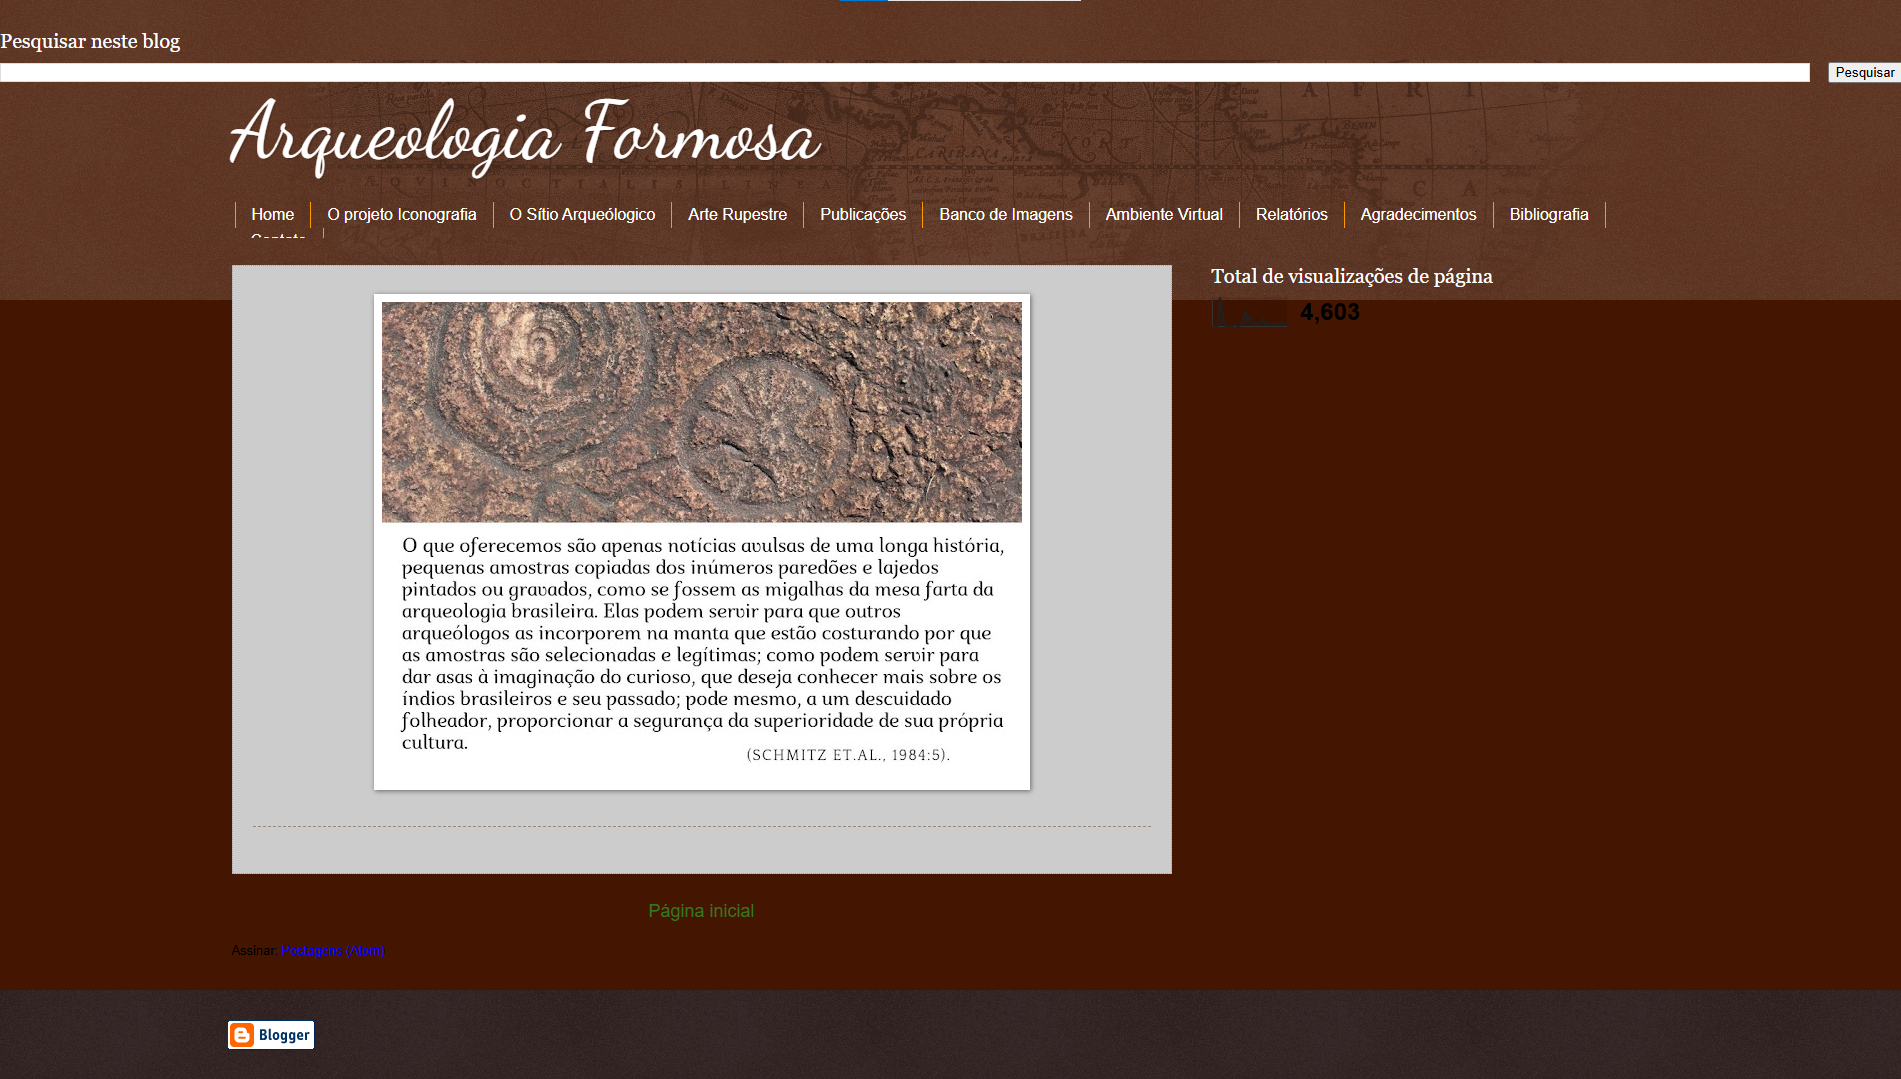
\includegraphics[width=1\linewidth]{images/home-blog-print.png}
    \caption{Captura de tela da página inicial do blog \href{https://arqueologiaformosa.blogspot.com/}{"Arqueologia Formosa"}}
    \label{fig:Captura de tela da página inicial do blog}
\end{figure}

\section{Objetivo Geral}
O objetivo deste trabalho é desenvolver uma plataforma web e um ambiente virtual \gls{3d} que permitam a preservação, divulgação e o acesso à arte rupestre da Lapa da Pedra. Esse projeto busca oferecer uma experiência interativa para educadores, pesquisadores e o público em geral, promovendo a conscientização sobre a importância desses registros culturais.

\section{Objetivos Específicos}
Os objetivos específicos do projeto incluem:
\begin{itemize}
    \item Realizar uma análise heurística de usabilidade do antigo site "Arqueologia Formosa", a fim de identificar possíveis melhorias que otimizem a experiência do usuário e garantam uma navegação mais intuitiva e acessível.
    \item Desenvolver um novo site com um design centrado na experiência do usuário, do inglês, \gls{ux}, oferecendo navegação e acessibilidade aprimoradas.
    \item Implementar um ambiente virtual \gls{3d} que permita a visualização interativa da arte rupestre encontrada na Lapa da Pedra e disponibilizar para \textit{download} no site desenvolvido.
\end{itemize}


\section{Justificativa}
A relevância deste estudo está intrinsecamente relacionada à crescente importância da arqueologia virtual como uma ferramenta eficaz para a preservação e estudo do patrimônio arqueológico em um mundo que enfrenta desafios contínuos em relação à degradação dos sítios históricos. Neste contexto, tecnologias digitais não só oferecem uma nova forma de interagir com o passado, mas também permitem a democratização do acesso a elementos culturais. Por exemplo, projetos semelhantes têm demonstrado que a virtualização de artefatos históricos pode aumentar a conscientização e o respeito pelas culturas que moldaram nossa história.

Por outro lado, a criação de um ambiente digital para a preservação cultural traz inúmeras vantagens tanto para a educação quanto para a pesquisa, possibilitando o acesso a informações e experiências que, de outra forma, seriam limitadas. Além disso, a experiência prévia adquirida pelo autor no \gls{PIBIC} intitulado "Iconografia e Arte Rupestre Formosense: Criação de um Banco de Imagens e Modelos \gls{3D} da Lapa da Pedra" \footnote{Disponível para leitura em: 
\href{https://drive.google.com/file/d/1Id44ViPFScX0Z1TIxGngs4_7UXPabMDt/view?usp=sharing}{https://drive.google.com/file/d/1Id44ViPFScX0Z1TIxGngs4_7UXPabMDt/view?usp=sharing} *\textbf{ COLOCAR LINK DO SICT QUANDO FOR PUBLICADO}}, sob a orientação do professor de Artes do \gls{IFG}, Edson Rodrigues Borges, enriqueceu significativamente a compreensão dos processos de fotogrametria e da criação de modelos \gls{3D} aplicados à arqueologia formosense. Com isso, esse conhecimento se torna fundamental para a implementação deste projeto, ao expandir e aprimorar o acesso a esses recursos digitais.

Dessa forma, esta pesquisa não apenas contribui para o avanço da arqueologia virtual, mas também possui implicações significativas na valorização e proteção do patrimônio cultural. Ao tornar acessíveis as pinturas rupestres da Toca da Onça a um público mais amplo, busca-se não só promover o conhecimento e a apreciação destes tesouros históricos, mas também engajar a sociedade na sua preservação, incentivando a reflexão sobre a identidade cultural e a herança coletiva que todos compartilhamos.

\section{Descrição dos Capítulos}
Os próximos capítulos deste trabalho são organizados da seguinte forma:
\begin{itemize}
    \item \textbf{Referencial Teórico}
    Dedica-se à fundamentação teórica do trabalho e aos principais conceitos e termos do trabalho, para que o leitor possa ter leitura fluida e compreensão integral do que está lendo. O capítulo aborda sobre a arqueologia e a arte rupestre, com foco no sítio Lapa da Pedra e nas ameaças à sua preservação. Discute o conceito de patrimônio virtual e suas aplicações, além dos métodos de fotogrametria, modelagem \gls{3d}, e práticas de engenharia de software e desenvolvimento web, com ênfase em Experiência do Usuário. Apresenta também as ferramentas utilizadas.
    
    \item \textbf{Método}: Explica o planejamento, a metodologia escolhida, a coleta de requisitos, o desenvolvimento do sistema, incluindo o uso de Kanban, a criação do ambiente virtual e o desenvolvimento do novo site.
    
    Descreve o processo de desenvolvimento adotado, incluindo a forma de organização das atividades (por exemplo, Kanban) e a coleta de requisitos. Expõe também a modelagem de dados e a arquitetura geral do sistema, explicando como cada componente foi planejado para atender aos objetivos.
    
    \item \textbf{Desenvolvimento}: Foca na implementação prática do projeto. Apresenta a construção do site com Next.js e Sanity, a integração com serviços externos (Flickr, Google Drive, Sketchfab) e, em seguida, o desenvolvimento do ambiente virtual na Unreal Engine, detalhando desde a 
    fotogrametria até a disponibilização do executável.
    
    \item \textbf{Resultados}: Descreve os produtos finais obtidos, comparando o novo site e o ambiente virtual com as versões anteriores.
    \item \textbf{Conclusão}: Resume os principais resultados alcançados, limitações encontradas e sugestões para trabalhos futuros.
    \item \textbf{Referências}: Lista as obras, artigos e demais fontes bibliográficas consultadas para embasar o trabalho.
    \item \textbf{Apêndice}: Reúnem materiais de apoio que não cabem no corpo principal, mas enriquecem o trabalho. Estão inclusos o questionário de requisitos, registros de reuniões, e demais documentos que auxiliam na compreensão detalhada do trabalho.


\end{itemize}


\chapter{Referencial Teórico}
\label{Referencial_Teorico}

\section{Arqueologia}%
A arqueologia é a ciência que estuda as culturas humanas através da recuperação, análise e interpretação dos vestígios materiais deixados por essas sociedades ao longo do tempo. Esses vestígios podem incluir artefatos, edificações, utensílios, entre outros elementos materiais que fornecem informações valiosas sobre os modos de vida, as práticas sociais e as organizações econômicas e políticas dos povos antigos. Conforme destaca \cite{funari2024arqueologia}, a arqueologia é essencial para a compreensão da história da humanidade, pois complementa e enriquece os dados obtidos por outras disciplinas, como a história e a antropologia, permitindo uma visão mais abrangente e detalhada das sociedades passadas. Assim, ao explorar os vestígios materiais, os arqueólogos contribuem significativamente para a reconstrução e preservação da memória coletiva, além de promover a valorização do patrimônio cultural.
Ao falar de arqueologia podemos nos deparar com várias formas de expressão, como por exemplo, a arte rupestre.
\subsection{Arte Rupestre}
%Falar sobre a definição(que é mais geral), falar sobre a toca da onça. sobre pictoglifos(que são as pinturas).



O termo “rupestre” tem origem no latim "rupestris”, derivado de “rupes”, que significa "rocha" ou “penhasco”. Assim, define-se como "Arte Rupestre” toda expressão gráfica, seja gravura ou pintura, que utiliza como suporte uma superfície rochosa, independentemente de suas características e dimensões \cite[p. 7]{pedroignacioschmitz_1984_arte}. As paredes de abrigos, grutas, penhascos e até mesmo rochas isoladas se transformam em telas para essas manifestações ancestrais.
Existem dois principais tipos de arte rupestre:
\begin{itemize}
\item \textbf{Pintura Rupestre (Pictografia):} Criação de imagens utilizando pigmentos minerais, vegetais ou animais, aplicados diretamente na superfície rochosa.
\item \textbf{Gravura Rupestre (Petróglifo):} Produção de desenhos através do desgaste da superfície rochosa, utilizando ferramentas líticas, como pedras pontiagudas.
\end{itemize}
A arte rupestre, presente em diversas partes do mundo, representa uma das formas mais antigas de expressão humana, oferecendo informações valiosas sobre as culturas que as produziram (MARQUES, 2016).

\subsection {Sítio Arqueológico Lapa da Pedra}\label{sec:sitio lapa da pedra}
O Sítio Arqueológico Lapa da Pedra, mostrado na Figura \ref{fig:Entrada da Gruta IV,Toca da Onça}, é conhecido popularmente como Toca da Onça fica localizado em uma fazenda de propriedade privada a nordeste de Formosa, chamada fazenda Pedra. Na Figura \ref{fig:mapa} pode-se observar o mapa e o caminho percorrido. Em 1984, Pedro Ignácio Schmitz e Altair Sales Barbosa realizaram pesquisas que culminaram na identificação e catalogação de 29 pequenas grutas na região de Formosa, Goiás. Essas grutas abrigavam pinturas rupestres e serviram como moradia para os primeiros habitantes do cerrado (BARBOSA et al., 1984, 1993). 
Dentre as 29 grutas, a Gruta catalogada por Schmitz como IV–GO-EC-002 (04), se destaca pela maior concentração de pictoglifos e, portanto, foi o foco da virtualização neste trabalho. Localizada a cerca de 12 km da cidade de Formosa, a Gruta 04 consiste em uma passagem de duzentos metros abaixo de uma enorme pedra calcária, situada na fazenda Pedra. Esse sítio, semelhante a outros em Goiás e no noroeste de Minas Gerais, apresenta uma grande diversidade de temas na arte rupestre, datando de aproximadamente 4.560 a.C. (SCHMITZ, 1990).


\begin{figure}[H]
    \centering
    \includegraphics[height=11cm, keepaspectratio]{img/Entrada Gruta IV Toca da Onça.jpeg}
    \caption{Entrada da Gruta IV, Toca da Onça. \\
        \textbf{Fonte:} Elaborado pelo autor.}
    \label{fig:Entrada da Gruta IV,Toca da Onça}
\end{figure}

\begin{figure}[H]
    \centering
    \includegraphics[height=8cm, keepaspectratio]{img/Visitas tecnicas/mapa.png}
    \caption{ Diagrama em cima da captura de tela do Google Earth \\ na localização das grutas da Lapa da Pedra. Captura de tela realizada em junho de 2024 \\
        \textbf{Fonte:} Elaborado pelo autor.}
    \label{fig:mapa}
\end{figure}


\subsection{Ameaças à Preservação da Arte Rupestre: Deteriorização e Ação Antrópica}\label{sec:amecas a preservação}
A arte rupestre, como patrimônio cultural de valor inestimável, enfrenta diversos desafios para sua preservação. A ação do tempo e as condições climáticas, como a umidade, a luz, o calor e o vento, contribuem para a deterioração natural das pinturas e superfícies rochosas.
Na Toca da Onça,  não bate sol dentro da gruta, contribuindo para a preservação do estado dos desenhos. Contudo, ainda se observam fatores de deterioração natural: descamação da tinta, infiltrações, fissuras nas rochas.


Além da deterioração natural, a ação antrópica, que se configura como a interferência humana no ambiente, representa uma grave ameaça à preservação da arte rupestre. Vandalismo, turismo desordenado, contato direto com as pinturas, poluição e obras próximas aos sítios arqueológicos podem causar danos irreversíveis a este patrimônio.
Em relação à Toca da Onça, os seguintes exemplos de impactos causados pela ação antrópica foram notados: vandalismo, pichações, degradação causada pelo turismo desordenado, fotos com \textit{flash}. Como por exemplo o que pode ser observado na Figura \ref{fig:degradacao_toca_onca}.

\begin{figure}[H]
    \centering
    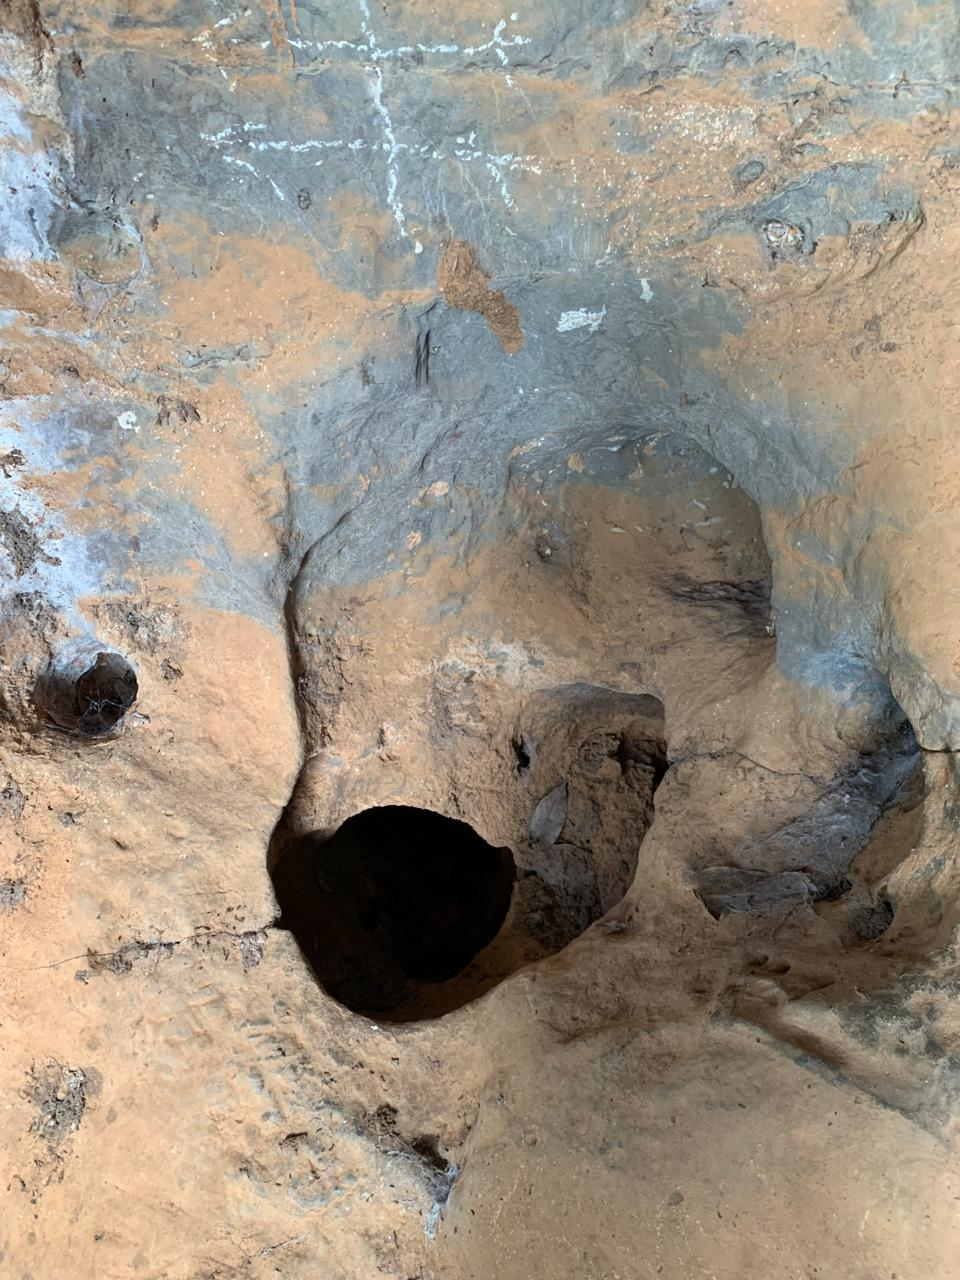
\includegraphics[height=11cm, keepaspectratio]{img/jogo da velha.jpeg}
    \caption{Depredação do Patrimônio na Toca da Onça. \\
        \textbf{Fonte:} Elaborado pelo autor.}
    \label{fig:degradacao_toca_onca}
\end{figure}


\section{Patrimônio Virtual (Virtual Heritage)}
\subsection{Conceitos e Importância}
Discutir o conceito de patrimônio virtual e seu impacto na arqueologia.

Diante dos desafios para a preservação da arte rupestre, a virtualização 3D surge como uma ferramenta poderosa para documentar, estudar e divulgar este importante patrimônio cultural, minimizando os impactos causasdos da visitação aos sítios arqueológicos.

\subsection{Aplicações em Arqueologia}
Dar exemplos de como o patrimônio virtual tem sido usado para preservar sítios históricos.




\section{Fotogrametria e Modelagem 3D}\label{sec:fotogrametria e modelagem 3D}
Para construção de um Patrimônio Virtual com qualidade é preciso construir modelos 3D fidedignos a realidade e para isso existe uma técnica muito utilizada chamada fotogrametria.
A fotogrametria, deriva das raízes gregas “photós” (luz), “gramma” (desenhado ou escrito) e “metria” (medição). Logo, fotogrametria etimologicamente significa “medições gráficas por meio da luz" (Paredes, 1987). A American Society for Photogrammetry and Remote Sensing (ASPRS), em seu livro The Manual of Photogrammetry (2003), define fotogrametria como “a arte, ciência e tecnologia de obter informações confiáveis sobre objetos físicos e o ambiente por meio de processos de registro, medição e interpretação de imagens fotográficas e padrões de energia radiante eletromagnética (EM) e outros fenômenos.”
Historicamente, a fotogrametria  teve seu desenvolvimento intrinsecamente ligado à evolução da fotografia, da óptica e da geometria, culminando em uma ferramenta crucial para diversos campos do conhecimento. No Brasil, sua história acompanha de perto a evolução global, com momentos de pioneirismo e adaptação às demandas nacionais (Silva, 2015).

Quanto a sua evolução, a fotogrametria passou por quatro fases principais: a Fotogrametria de Tábua Plana (1850–1900), iniciada por A. Laussedat com o uso de fotografias terrestres para mapeamento (Silva e Borges, 2023); a Fotogrametria Analógica (1900–1950), que incorporou a estereoscopia e fotografias aéreas para fins topográficos; a Fotogrametria Analítica (1950-1990), que otimizou os processos com a introdução de computadores e automatização; e a Fotogrametria Digital (1990-atualmente), caracterizada por processos automáticos realizados em computadores, além da popularização de câmeras digitais de alta qualidade que simplificam o processo (Borges e Silva, 2023).

A criação de um modelo 3D com fotogrametria digital, como descrito por Linhares e Groetelaars (2021), envolve um processo que se inicia com o planejamento do levantamento, definindo os objetivos, escolhendo o equipamento adequado e planejando a tomada fotográfica. A etapa seguinte, como apresentado por Groetelaars (2004), é a aquisição de dados no campo, que consiste na captura de fotografias e na medição das coordenadas dos pontos de controle no espaço real, utilizando métodos topográficos ou 3D Laser Scanning. Após a aquisição, o processamento dos dados é realizado por softwares específicos, que orientam as imagens interna e externamente com base nos pontos de controle, gerando uma nuvem de pontos densa. A partir dessa nuvem, o software cria uma malha triangular irregular (TIN), que representa a forma do objeto e pode ser texturizada com as imagens originais. A etapa final envolve o pós-processamento para remover ruídos, \textit{outliers} e falhas, otimizar a malha e aplicar texturas, resultando em um modelo 3D fotorrealístico.
A fotogrametria automatizada, comumente empregada na geração de modelos 3D de sítios arqueológicos, envolve um processo que se inicia com a captura de imagens de alta qualidade, utilizando câmeras terrestres ou aéreas com sobreposição e georreferenciamento por meio de pontos de controle (GCPs) (McGlone, 2004). O software realiza o alinhamento das imagens, corrigindo distorções geométricas e determinando a posição e orientação de cada fotografia no espaço. Através da correlação de imagens, o software identifica pontos correspondentes e calcula as coordenadas 3D de cada ponto, gerando uma nuvem densa de pontos 3D (Heipke, 2001). A partir da nuvem de pontos, o software gera modelos 3D, atribui texturas e corrige distorções geométricas, produzindo modelos 3D precisos e realistas do sítio arqueológico (Gruen, 2008). A geração de modelos 3D permite a documentação detalhada do sítio, a análise tridimensional da estrutura e a criação de representações visuais para estudos e divulgação científica.


%\subsection{Engine}
\subsection{Unreal Engine}No contexto do desenvolvimento de jogos e aplicações interativas, a \textit{engine} desempenha um papel fundamental como a espinha dorsal tecnológica. Uma \textit{engine} de jogo é um conjunto complexo de bibliotecas de software que fornece aos desenvolvedores um arcabouço completo para criar e alimentar experiências interativas em tempo real. Essas ferramentas abrangem desde a renderização gráfica e simulação de física até a inteligência artificial, interface do usuário e gerenciamento de áudio. Sem uma \textit{engine}, os desenvolvedores precisariam construir todas essas funcionalidades do zero, tornando o processo de desenvolvimento significativamente mais complexo e demorado. 

A \textit{Unreal Engine}, desenvolvida pela\textit{ Epic Games}, se destaca como uma \textit{engine} de jogos de última geração, amplamente utilizada na indústria de jogos e simulações, e reconhecida por sua capacidade de criar experiências visuais de alta qualidade e interativas.  A \textit{Unreal Engine} oferece um conjunto robusto de ferramentas para modelagem 3D, animação, física, renderização, iluminação, realidade virtual e muito mais. Sua arquitetura flexível e código-fonte aberto permitem que os desenvolvedores personalizem e estendam a \textit{engine} para atender às necessidades específicas de seus projetos, tornando-a uma escolha popular tanto para grandes estúdios quanto para desenvolvedores independentes.

No âmbito do Patrimônio Virtual, a \textit{Unreal Engine} se torna uma ferramenta poderosa para a criação de reconstruções digitais imersivas e interativas de sítios arqueológicos, monumentos e artefatos históricos. A \textit{engine} permite a modelagem 3D realista, a aplicação de texturas detalhadas e a simulação precisa de iluminação, proporcionando aos usuários uma experiência virtual imersiva e próxima da realidade. A capacidade de integrar elementos interativos, como navegação em primeira pessoa, animações e informações contextuais, enriquece ainda mais a experiência, tornando a \textit{Unreal Engine} uma escolha estratégica para projetos que buscam aproximar o público do patrimônio cultural.

\subsection{RealityCapture e Integração com Unreal Engine}
O \textbf{RealityCapture}, desenvolvido pela CapturingReality e adquirido pela Epic Games, é amplamente utilizado para a criação de modelos 3D altamente detalhados a partir de técnicas de fotogrametria. Uma das principais vantagens do RealityCapture é sua integração nativa com a Unreal Engine, também desenvolvida pela Epic Games. Essa compatibilidade facilita a exportação de modelos 3D para a Unreal Engine, onde podem ser utilizados na criação de ambientes virtuais realistas, como em jogos, simulações ou experiências de realidade virtual (VR) \citep{EpicGamesDocs}.

A integração entre o RealityCapture e a Unreal Engine é particularmente útil em projetos de patrimônio cultural, onde a reconstrução digital de sítios arqueológicos ou artefatos pode ser visualizada em ambientes virtuais interativos. Essa combinação permite a criação de experiências imersivas, como visitas virtuais a museus ou sítios históricos, com um alto nível de realismo e detalhamento \citep{ExemploArtigo}.
\subsection{Metahumans}

A representação humana em ambientes virtuais tem papel crucial na criação de experiências imersivas e relacionáveis. No contexto do Patrimônio Virtual, a presença de personagens virtuais humanoides pode auxiliar na comunicação de narrativas históricas, guiar usuários por sítios arqueológicos reconstruídos e demonstrar costumes e atividades do passado. Nesse sentido, a ferramenta \textit{MetaHuman Creator} (Figura \ref{fig:metahuman creator}), da Epic Games, surge como um recurso poderoso para a criação de avatares digitais de alta fidelidade.
O \textit{MetaHuman Creator} permite a geração e personalização de rostos e corpos humanos com alto nível de realismo, incluindo detalhes como textura de pele, cabelo, expressões faciais e diferentes tipos de corpo. A interface intuitiva e a ampla gama de opções de personalização permitem a criação de personagens únicos e específicos, evitando a aparência genérica frequentemente associada a avatares digitais. Esse recurso permite a criação detalhada de personagens realistas que podem ser integrados em simulações e experiências interativas, enriquecendo a representação do patrimônio cultural, tornando-a mais próxima e humanizada.

\begin{figure}[H]
    \centering
    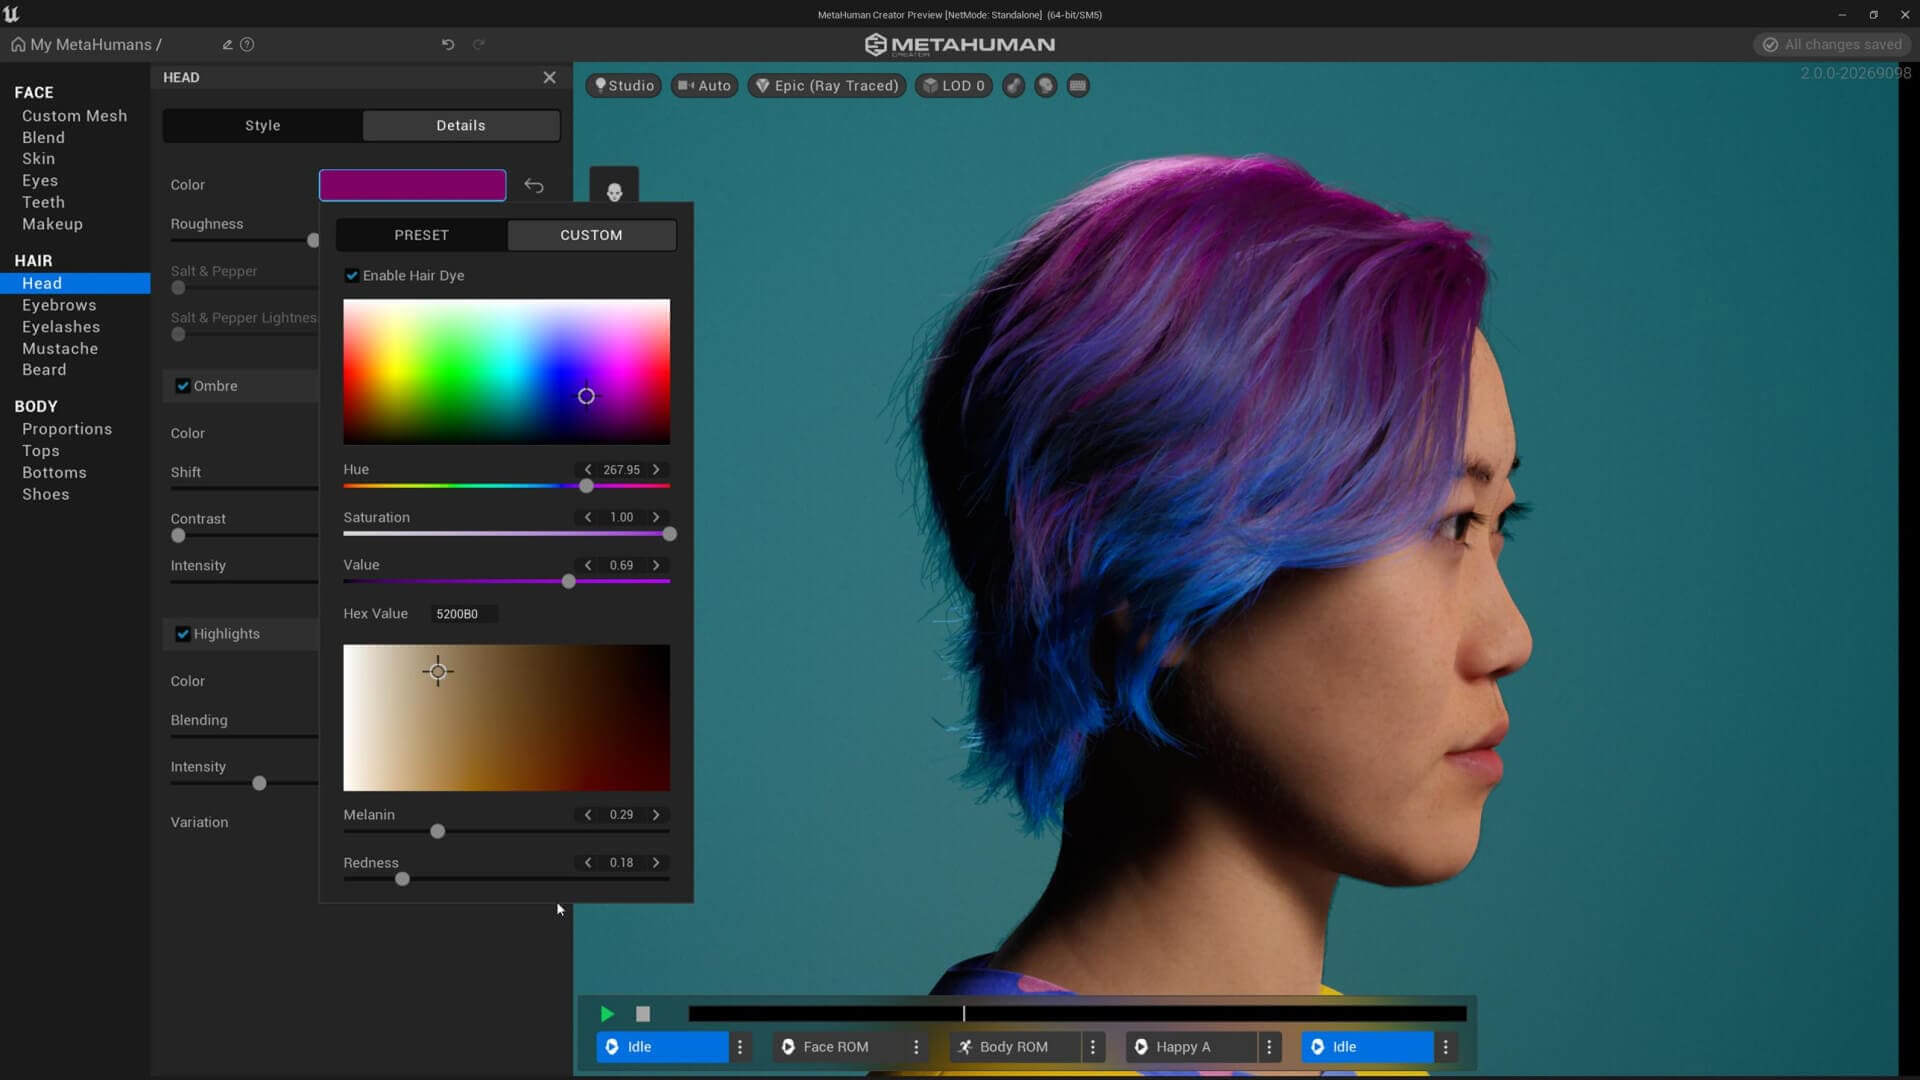
\includegraphics[height=8cm, keepaspectratio]{img/unreal/metahuman create.jpg}
    \caption{Editor da Plataforma MetaHuman \\
        \textbf{Fonte:} \href{https://cdn2.unrealengine.com/metahuman-overview-create-1920x1080-baa630fe8b02.jpg?resize=1&w=900}{Unreal Engine - MetaHumans},  \protect\citep{unrealenginemeta}}
    \label{fig:metahuman creator}
\end{figure}

Um aspecto fundamental para a integração convincente de Metahumans em ambientes virtuais é a animação. Cada \textit{MetaHuman} possui um "esqueleto digital" interno, uma estrutura articulada que permite a aplicação de movimentos, como mostrado na Figura \ref{fig:skeleton}. Através da importação de animações pré-definidas, que podem ser vistas na Figura \ref{fig:animacoes}, ou da criação de animações personalizadas utilizando softwares de animação 3D, é possível atribuir aos Metahumans ações como andar, correr, pular, gesticular e interagir com objetos no ambiente virtual. A fluidez e naturalidade dessas animações são essenciais para garantir a imersão do usuário e a credibilidade da representação.

\begin{figure}[H]
    \centering
    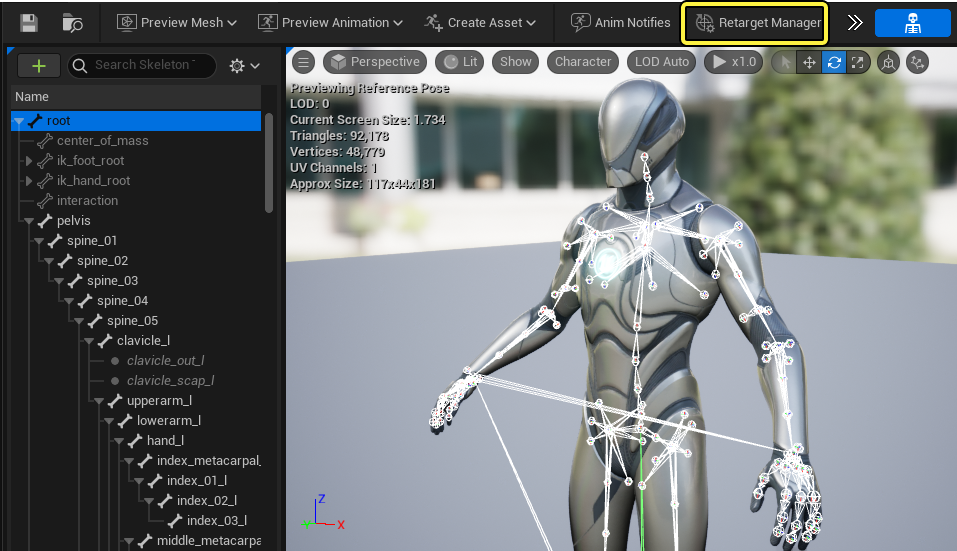
\includegraphics[height=8cm, keepaspectratio]{img/skeleton.png}
    \caption{Captura de tela do Esqueleto digital \\de um avatar na Unreal Engine.\\
        \textbf{Fonte:} Elaborado pelo autor.}
    \label{fig:skeleton}
\end{figure}

\begin{figure}[H]
    \centering
    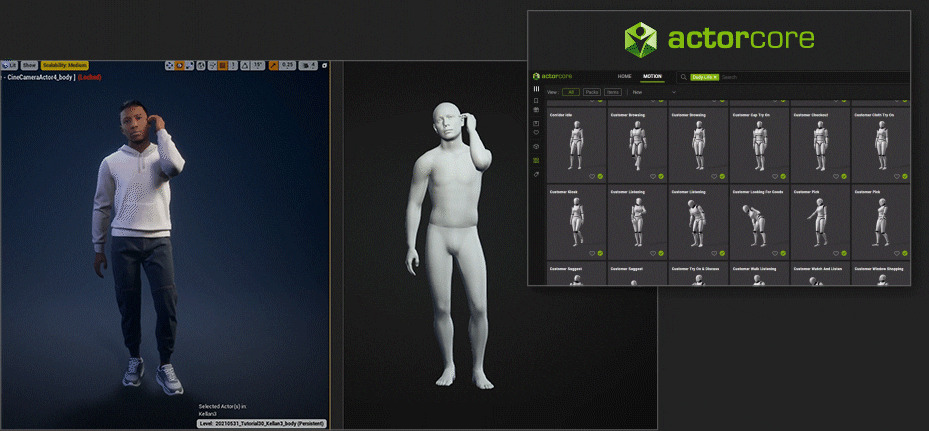
\includegraphics[height=8cm, keepaspectratio]{gif/animacoes/feature_body_motion-0000.jpg}
    \caption{ Captura de tela do pacote de animações Unreal.\\
        \textbf{Fonte:} Elaborado pelo autor.}
    \label{fig:animacoes}
\end{figure}


A Figura \ref{fig:metahumanEdson} ilustra a aplicação da tecnologia MetaHuman na representação do Professor Edson, profissional da área de artes e entusiasta da arqueologia. O modelo digital, criado a partir de fotografias como referência, captura suas características físicas com fidelidade, demonstrando o potencial da ferramenta na criação de representações personalizadas. A utilização de um MetaHuman com a aparência do Professor Edson em uma experiência de Patrimônio Virtual permite, por exemplo, que ele atue como um guia virtual, conduzindo os usuários por um sítio arqueológico reconstruído, fornecendo explicações e respondendo a perguntas, criando assim uma experiência mais interativa e humanizada.

\begin{figure}[H]
    \centering
    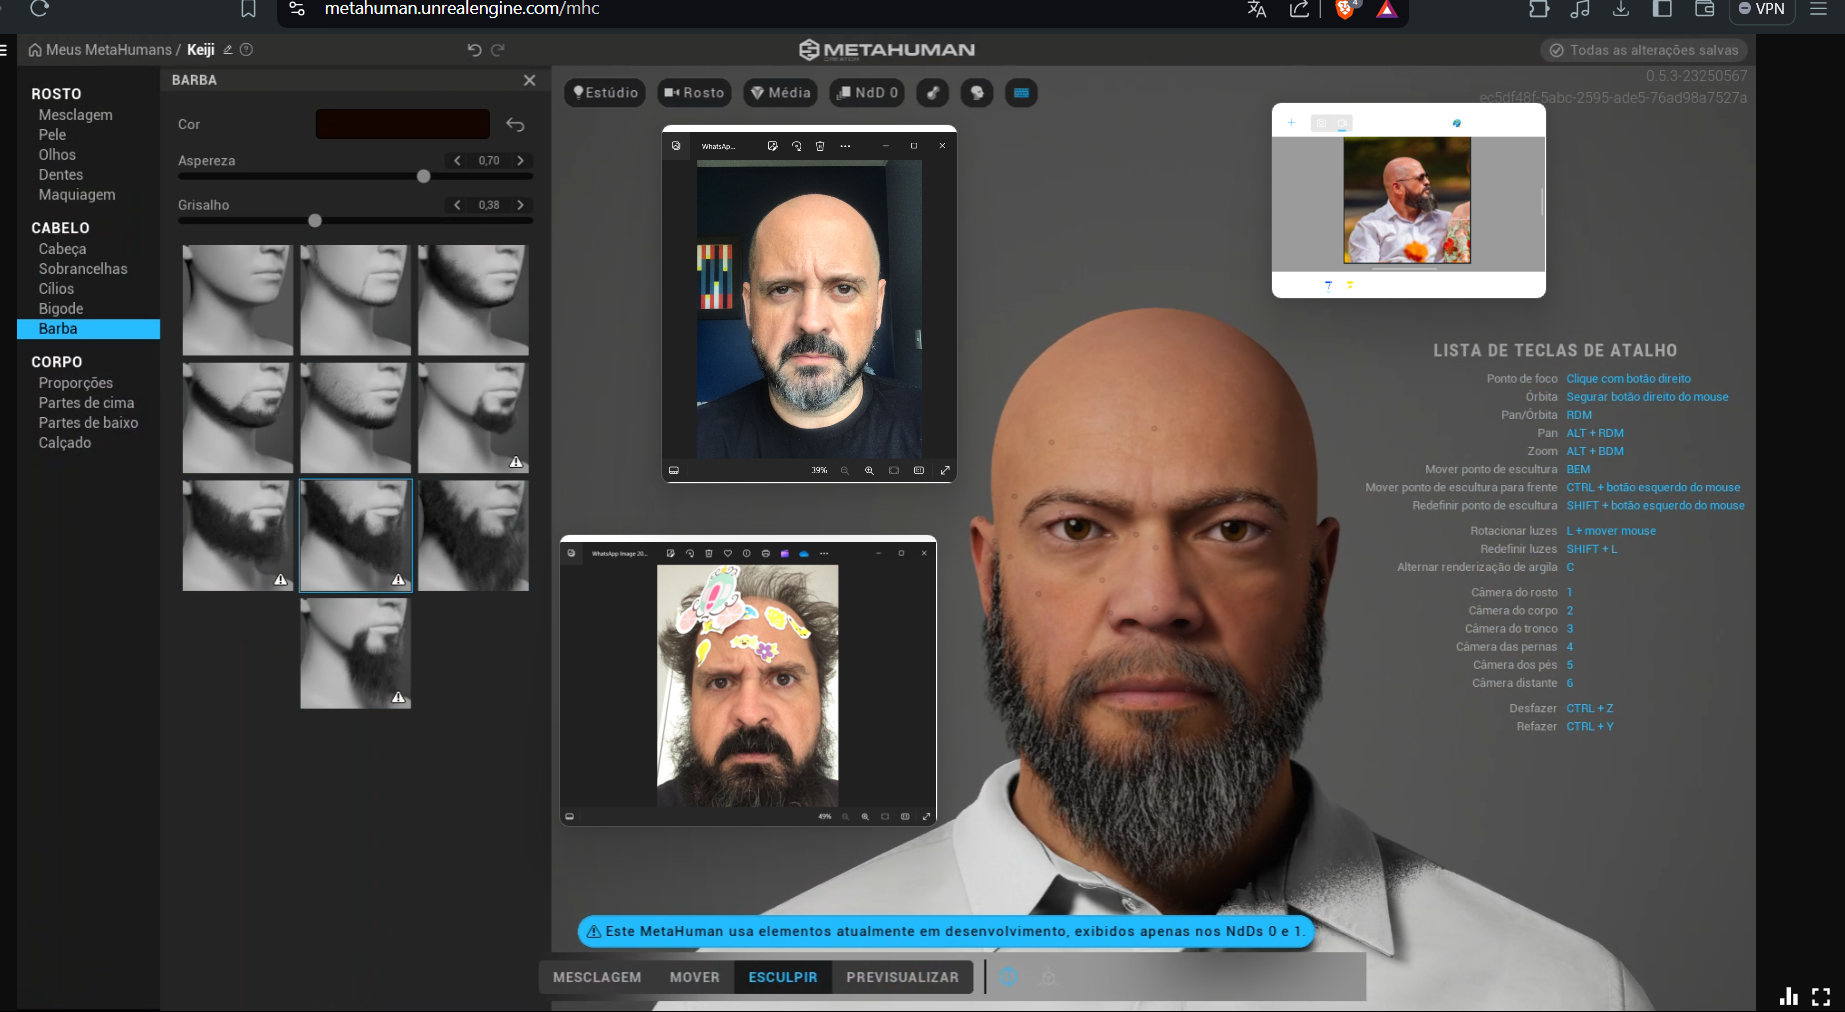
\includegraphics[height=8cm, keepaspectratio]{img/Metahuman.png}
    \caption{Criação do Avatar Digital do professor Edson Borges. \\
        \textbf{Fonte:} Elaborado pelo autor.}
    \label{fig:metahumanEdson}
\end{figure}



A capacidade de gerar personagens virtuais realistas e personalizáveis, combinada com a possibilidade de animá-los de forma natural e convincente, torna os Metahumans uma ferramenta poderosa para a criação de experiências imersivas e envolventes no campo do Patrimônio Virtual. A presença de personagens virtuais humanoides pode contribuir significativamente para a comunicação de narrativas históricas.

\section{Engenharia de Software}
% \subsection{Modelos de Processo}
% Discutir diferentes modelos de processo de desenvolvimento de software, como Cascata, Agile, etc.

\subsection{UML: Unified Modeling Language}
A Unified Modeling Language (UML) é uma linguagem de modelagem amplamente utilizada para visualizar, especificar, construir e documentar artefatos de sistemas de software \citep{Booch2005}. Criada por Grady Booch, James Rumbaugh e Ivar Jacobson, a UML oferece um conjunto de diagramas padronizados que auxiliam no entendimento e na comunicação entre equipes de desenvolvimento. Segundo \cite{Booch2005}, a UML é composta por diagramas estruturais (como Diagramas de Classe e de Objetos) e comportamentais (como Diagramas de Caso de Uso e de Sequência), que permitem representar diferentes perspectivas de um sistema.

A UML tem sido fundamental para a engenharia de software, especialmente no contexto de desenvolvimento orientado a objetos. Conforme destacado por \cite{Fowler2005}, a linguagem é flexível o suficiente para ser adaptada a diferentes metodologias de desenvolvimento, como o Rational Unified Process (RUP) e métodos ágeis. Além disso, a UML é mantida e atualizada pela Object Management Group (OMG), garantindo sua evolução contínua para atender às necessidades da indústria de software.

\subsection{Cenário de Caso de Uso}
Um cenário de caso de uso é uma descrição detalhada de uma sequência de interações entre um usuário (ou ator) e um sistema para alcançar um objetivo específico. Esses cenários são fundamentais na engenharia de software, pois ajudam a identificar e esclarecer os requisitos do sistema, garantindo que todas as possíveis interações sejam consideradas durante o processo de desenvolvimento \citep{pressman2021engenharia}.

\subsection{Requisitos Funcionais}
Requisitos funcionais especificam as funções que um sistema deve executar, descrevendo as entradas, comportamentos e saídas esperadas. Eles definem o que o sistema deve fazer para atender às necessidades dos usuários e são essenciais para orientar o desenvolvimento e a validação do software \citep{pressman2021engenharia}.

\subsection{Requisitos Não Funcionais}
Requisitos não funcionais referem-se às características de qualidade que o sistema deve possuir, como desempenho, segurança, usabilidade, confiabilidade e escalabilidade. Eles estabelecem restrições e critérios que influenciam a experiência do usuário e a eficácia do sistema, garantindo que o software atenda a padrões de qualidade além das funcionalidades básicas \citep{pressman2021engenharia}.

\section{Desenvolvimento Web}

O desenvolvimento web é uma área da tecnologia responsável pela criação, codificação e programação de sites, aplicativos e seus respectivos sistemas, envolvendo tanto aspectos visuais quanto funcionais \citep{queirosintrodução}. Este campo desempenha um papel essencial na democratização do acesso à informação e serviços digitais, permitindo que empresas, instituições e indivíduos alcancem públicos globais por meio da internet.

De acordo com QUEIRÓS E PORTELA (2018), o desenvolvimento web pode ser dividido em três áreas principais: \textit{front-end}, \textit{back-end} e \textit{full-stack development}. O \textit{front-end} refere-se à interface do usuário, ou seja, tudo o que o usuário visualiza e interage diretamente no navegador. Já o \textit{back-end} lida com a lógica do servidor, gerenciamento de dados e integração com bancos de dados. O \textit{full-stack development}, por sua vez, combina ambas as áreas, permitindo que um desenvolvedor trabalhe em todas as camadas de uma aplicação web.

No contexto deste projeto, optou-se por utilizar tecnologias modernas que refletem as tendências atuais do desenvolvimento web. Para o \textit{front-end}, foi adotado um \textit{framework} que facilita a criação de interfaces dinâmicas e responsivas, melhorando significativamente o desempenho e a otimização para mecanismos de busca (SEO). No \textit{back-end}, utilizou-se uma solução de gerenciamento de conteúdo (\textit{headless CMS}) que permite maior flexibilidade no design e na entrega de conteúdo, separando a camada de apresentação da camada de dados.

Os autores destacam que o desenvolvimento web moderno exige uma abordagem global, considerando tanto os aspectos técnicos quanto a experiência do usuário \citeP{queirosintrodução}. Essa perspectiva guiou as escolhas tecnológicas deste trabalho, priorizando desempenho, acessibilidade e facilidade de manutenção.

\section{Experiência do Usuário (UX)}
A Experiência do Usuário (UX) é um conceito fundamental no design de sistemas interativos, focando na satisfação e na eficiência do usuário ao interagir com um produto ou serviço. Segundo \cite{Norman}, UX abrange todos os aspectos da interação do usuário com uma interface, desde a usabilidade até a experiência emocional.

\subsection{Heurísticas de Nielsen}
As heurísticas de Nielsen, propostas por Jakob Nielsen em 1994, são um conjunto de princípios amplamente utilizados para avaliar a usabilidade de interfaces. Essas heurísticas servem como diretrizes para identificar problemas de usabilidade e melhorar a interação do usuário. A seguir, são apresentadas as 10 heurísticas de Nielsen:

\begin{enumerate}
    \item \textbf{Visibilidade do Status do Sistema}: O sistema deve sempre manter os usuários informados sobre o que está acontecendo, por meio de feedback adequado e em tempo razoável. Por exemplo, barras de progresso ou mensagens de carregamento são formas de fornecer feedback.

    \item \textbf{Correspondência entre o Sistema e o Mundo Real}: O sistema deve falar a linguagem do usuário, com palavras, frases e conceitos familiares, em vez de termos técnicos. As informações devem aparecer em uma ordem natural e lógica.

    \item \textbf{Controle e Liberdade para o Usuário}: Os usuários frequentemente realizam ações por engano e precisam de uma "saída de emergência" claramente marcada para sair do estado indesejado. Isso inclui funcionalidades como "Desfazer" e "Refazer".

    \item \textbf{Consistência e Padrões}: Os usuários não devem se perguntar se palavras, situações ou ações diferentes significam a mesma coisa. Siga as convenções da plataforma e mantenha a consistência em todo o sistema.

    \item \textbf{Prevenção de Erros}: Um bom design evita que problemas ocorram. Isso pode ser feito eliminando condições propícias a erros ou verificando se há erros antes que o usuário confirme uma ação.

    \item \textbf{Reconhecimento em vez de Memorização}: Minimize a carga de memória do usuário, tornando objetos, ações e opções visíveis. O usuário não deve precisar lembrar informações de uma parte do sistema para outra.

    \item \textbf{Flexibilidade e Eficiência de Uso}: Aceleradores (como atalhos de teclado) podem aumentar a eficiência para usuários experientes, sem prejudicar a experiência de usuários iniciantes.

    \item \textbf{Estética e Design Minimalista}: As interfaces não devem conter informações irrelevantes ou raramente necessárias. Cada unidade extra de informação compete com as unidades relevantes e diminui sua visibilidade relativa.

    \item \textbf{Ajudar os Usuários a Reconhecer, Diagnosticar e Recuperar-se de Erros}: As mensagens de erro devem ser expressas em linguagem simples, indicar precisamente o problema e sugerir uma solução de forma construtiva.

    \item \textbf{Ajuda e Documentação}: Embora seja melhor que o sistema possa ser usado sem documentação, pode ser necessário fornecer ajuda e documentação. Essas informações devem ser fáceis de encontrar, focadas na tarefa do usuário e listar etapas concretas a serem seguidas.
\end{enumerate}

Essas heurísticas são amplamente utilizadas em avaliações de usabilidade, como inspeções heurísticas, para identificar problemas em interfaces e propor melhorias \citep{Nielsen1994}.

\subsubsection{Análise Heurística}
A \textbf{Análise Heurística} é um método de avaliação de usabilidade que consiste na inspeção sistemática de uma interface com base em um conjunto de princípios ou heurísticas predefinidas. Esse método é amplamente utilizado para identificar problemas de usabilidade em sites, aplicativos e outros sistemas interativos, sem a necessidade de envolvimento direto dos usuários \citep{Nielsen1994}.
Os principais objetivos da análise heurística envolvem identificar problemas de usabilidade que possam prejudicar a experiência do usuário; avaliar a conformidade da interface com princípios de design reconhecidos, como as heurísticas de Nielsen; propor melhorias que aumentem a eficiência, a satisfação e a acessibilidade do sistema.

O processo de análise heurística geralmente é composto pelas etapas de:

\begin{enumerate}
    \item \textbf{Seleção das Heurísticas}: Escolha um conjunto de heurísticas adequado ao contexto da avaliação, como as heurísticas de Nielsen.
    
    \item \textbf{Inspeção da Interface}: Um ou mais avaliadores examinam a interface, aplicando as heurísticas selecionadas para identificar problemas de usabilidade.
    
    \item \textbf{Documentação dos Problemas}: Cada problema identificado é documentado, descrevendo sua natureza, a heurística violada e, se possível, sugerindo uma solução.
    
    \item \textbf{Priorização e Relatório}: Os problemas são priorizados com base em sua gravidade e impacto na experiência do usuário, e um relatório detalhado é gerado para orientar as melhorias.
\end{enumerate}

\subsection{Web Content Accessibility Guidelines (WCAG)}

Outra coisa relacionada com a experiência de usuário é a acessibilidade, e para metrificar isso exitem as \textbf{Web Content Accessibility Guidelines (WCAG)}, desenvolvidas pelo \textbf{W3C}, que são padrões globais para acessibilidade digital, garantindo que interfaces sejam acessíveis a todos, incluindo pessoas com deficiências \citep{wcag21}. Organizadas em quatro princípios (\textbf{POUR}), as WCAG abordam:

\begin{itemize}
    \item \textbf{Perceivable (Perceptível)}: Conteúdo deve ser apresentado de forma acessível (ex.: alternativas textuais para imagens).
    \item \textbf{Operable (Operável)}: Interfaces devem ser navegáveis por teclado e compatíveis com tecnologias assistivas.
    \item \textbf{Understandable (Compreensível)}: Conteúdo e operação devem ser claros e previsíveis.
    \item \textbf{Robust (Robusto)}: Conteúdo deve ser compatível com diversas tecnologias.
\end{itemize}

As WCAG possuem três níveis de conformidade: \textbf{A} (mínimo), \textbf{AA} (recomendado) e \textbf{AAA} (ótimo). Sua adoção promove inclusão digital, conformidade legal e melhoria da experiência do usuário \citep{wcag21}.

% \subsection{Melhores Práticas}
% Discutir a relevância da acessibilidade, otimização para SEO e práticas comuns de segurança em aplicações web.


\section{JAMstack e Desenvolvimento Web Moderno}
\label{sec:jamstack}
A JAMstack é uma arquitetura moderna para desenvolvimento web que se baseia em três pilares principais: \textbf{JavaScript}, \textbf{APIs} e \textbf{Markup} \citep{jamstackorg}, como exemplificado na Figura \ref{fig:jamStack sigla}\footnote{Disponível em \href{https://cloudbytes.dev/snippets/what-is-jamstack-and-why-should-you-be-using-it}{https://cloudbytes.dev/snippets/what-is-jamstack-and-why-should-you-be-using-it}}. Essa abordagem promove a criação de sites rápidos, seguros e escaláveis, separando o front-end do back-end e utilizando serviços de terceiros para funcionalidades dinâmicas \citep{netlifyjamstack}.

\begin{figure}[H]
    \centering
    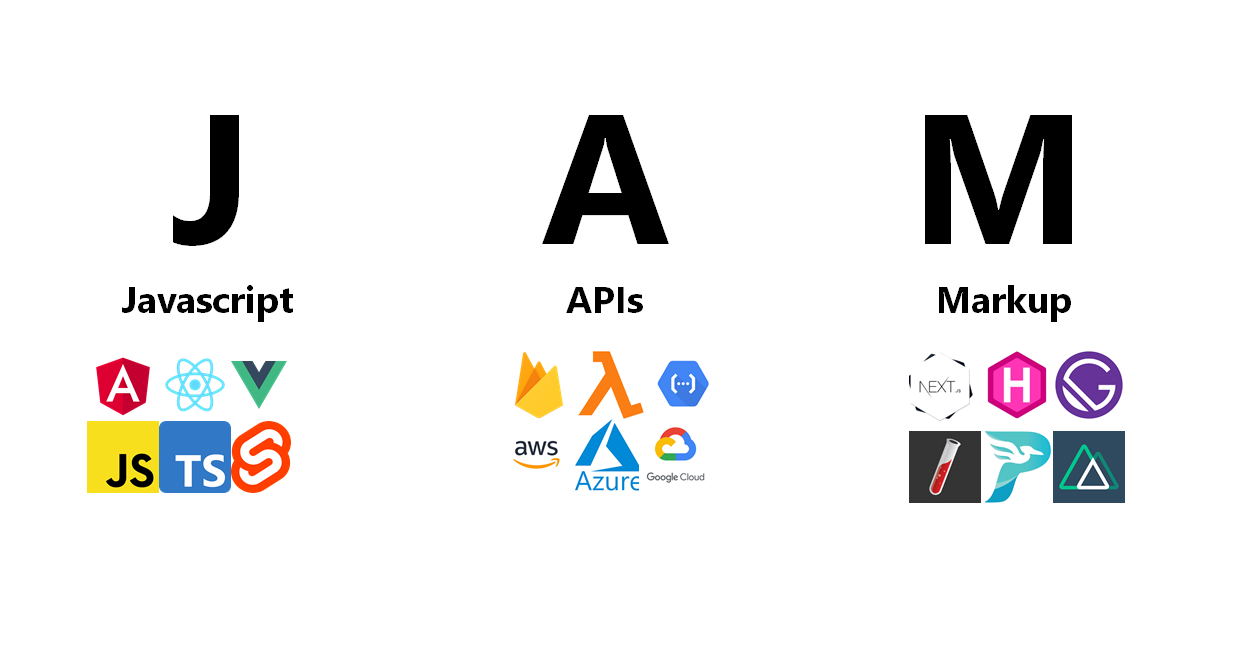
\includegraphics[height=8cm, keepaspectratio]{img/arquitetura/sigla JAM stack.png}
    \caption{ Significado da sigla JAM(Javascript, APIs e Markup)
 \\
        \textbf{Fonte:} Rehan Haider}
    \label{fig:jamStack sigla}
\end{figure}
De acordo com \cite{smashingmagazine}, a JAMstack tem ganhado popularidade devido à sua capacidade de simplificar o processo de desenvolvimento, permitindo que desenvolvedores se concentrem na experiência do usuário enquanto delegam tarefas complexas a APIs especializadas. Além disso, a pré-renderização de páginas estáticas contribui para uma melhor performance e segurança, reduzindo a superfície de ataque \citep{jamstackbook}.

A flexibilidade da JAMstack permite a integração com diversas ferramentas e serviços, como CMS headless, CDNs e ferramentas de automação, tornando-a uma escolha versátil para projetos de diferentes escalas \citep{netlifyjamstack}.

A arquitetura JAMstack (Figura \ref{fig:jamStack Arquitetura}) se destaca em relação a abordagens mais tradicionais, como o modelo de servidor monolítico e as arquiteturas baseadas em servidores dinâmicos. No modelo monolítico, todo o backend e frontend estão fortemente acoplados, exigindo que o servidor processe cada solicitação do usuário em tempo real. Isso pode gerar tempos de resposta mais lentos, especialmente em aplicações com alto tráfego, e torna mais difícil escalar ou implementar novas funcionalidades de maneira isolada.

\begin{figure}[H]
    \centering
    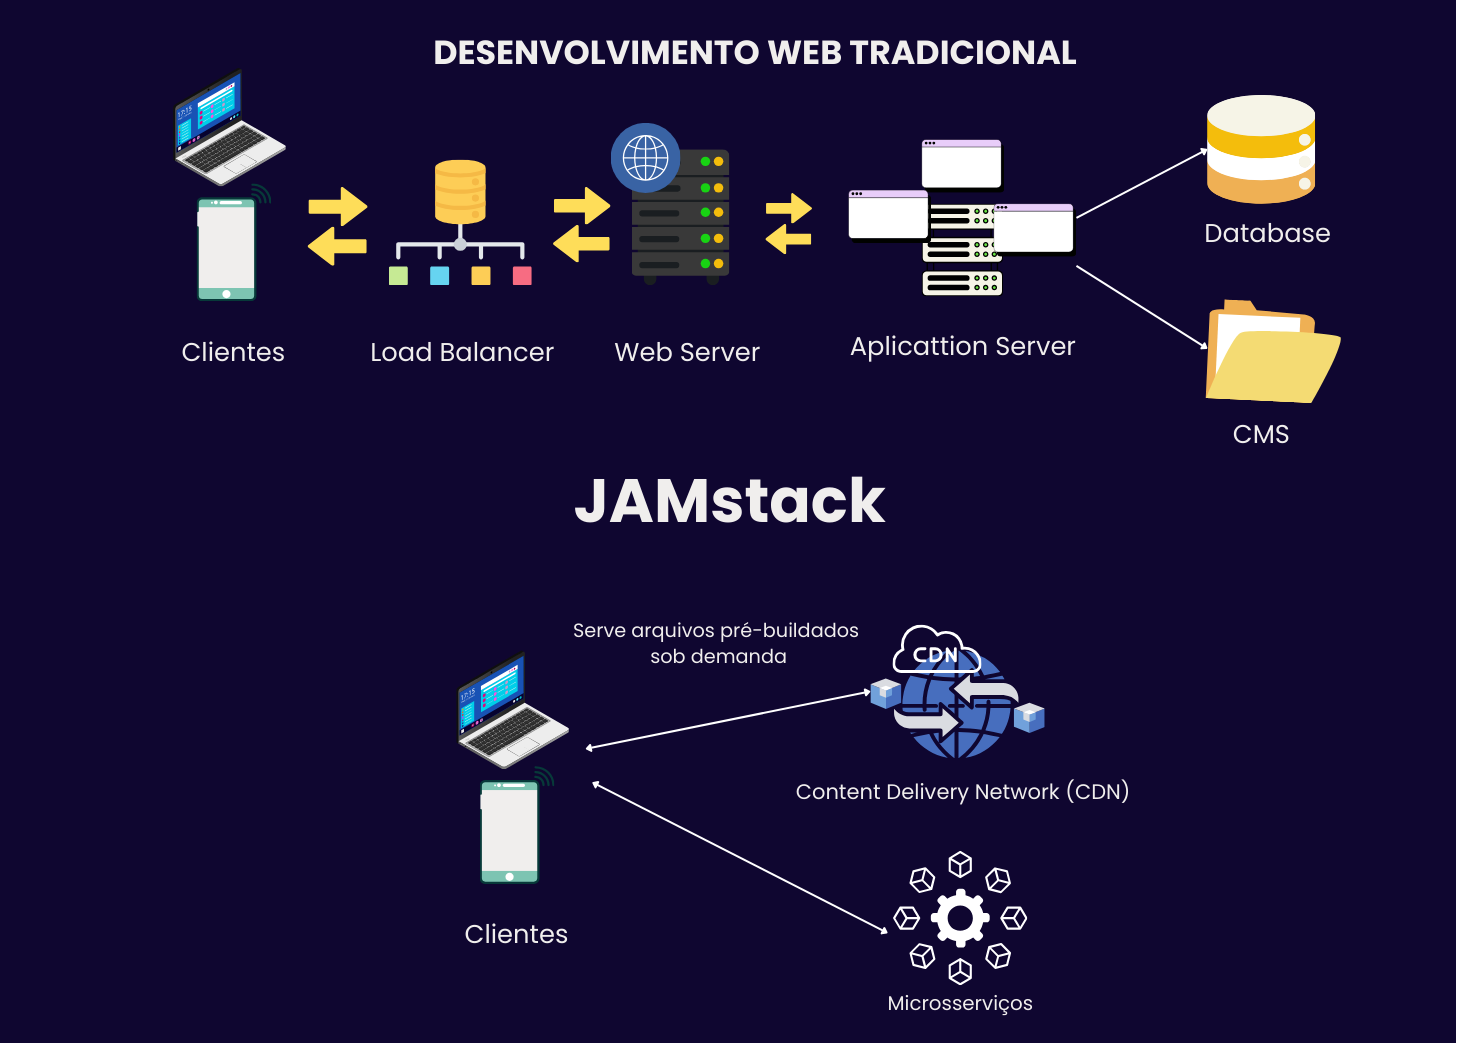
\includegraphics[height=8cm, keepaspectratio]{img/arquitetura/JAM STACK.png}
    \caption{ Comparação entre arquitetura tradicional e arquitetura JAMstack. \\
        \textbf{Fonte:} Elaborado pelo autor com base na documentação oficial do JAMstack.}
    \label{fig:jamStack Arquitetura}
\end{figure}

Já nas arquiteturas dinâmicas baseadas em servidores, como as utilizadas em sistemas gerenciadores de conteúdo tradicionais (ex.: WordPress), cada requisição ao site frequentemente aciona o servidor para buscar dados no banco e gerar a página no momento da requisição. Esse modelo pode causar problemas de performance e segurança, principalmente em picos de tráfego, além de depender de uma infraestrutura robusta para manter a operação.
Em contraste, a JAMstack evita a necessidade de renderização em tempo de execução, pré-gerando as páginas como arquivos estáticos no momento do build. Isso garante maior rapidez, segurança e escalabilidade, já que as páginas podem ser servidas diretamente por uma CDN sem passar por servidores intermediários. Além disso, ao desacoplar o frontend do backend, a JAMstack permite maior flexibilidade, facilitando a integração com APIs e serviços especializados, como sistemas de pagamento ou autenticação.
Por outro lado, a JAMstack apresenta limitações quando comparada a arquiteturas como microserviços ou serverless, que também oferecem modularidade e flexibilidade. Embora APIs desempenhem um papel fundamental na JAMstack, aplicações com lógica de negócios altamente complexa podem exigir um backend mais robusto, algo que arquiteturas serverless ou baseadas em microserviços conseguem oferecer de forma mais eficiente.

\section{Ferramentas Utilizadas}
Nesta seção, são apresentadas as principais ferramentas utilizadas no desenvolvimento deste trabalho, destacando suas funcionalidades e relevância para o projeto.

\subsection{Visual Studio Code}
O \gls{vs-code} é um editor de código-fonte desenvolvido pela Microsoft, amplamente utilizado por desenvolvedores devido à sua leveza, extensibilidade e suporte a diversas linguagens de programação. Ele oferece recursos como depuração integrada, realce de sintaxe, autocompletar inteligente e integração com ferramentas de controle de versão, como Git. Além disso, o VS Code possui um mercado de extensões que permite personalizar e expandir suas funcionalidades, tornando-o uma das ferramentas mais populares para desenvolvimento de software \citep{vscode}.

\subsection{Git e GitHub}
O Git é um sistema de controle de versão distribuído amplamente utilizado para rastrear alterações no código-fonte durante o desenvolvimento de software. Ele permite que desenvolvedores trabalhem em branches separados, facilitando a colaboração e a integração de mudanças. Já o GitHub é uma plataforma baseada em nuvem que hospeda repositórios Git, oferecendo funcionalidades adicionais como pull requests, issues e integração contínua. Juntos, Git e GitHub formam uma combinação poderosa para gerenciamento de projetos e colaboração em equipe \cite{git,github}.

\subsection{Notion}
 Notion é uma ferramenta de produtividade e organização que combina funcionalidades de notas, banco de dados, listas de tarefas e planejamento em uma única plataforma. Ele foi amplamente utilizado neste trabalho para a criação de quadros Kanban \footnote{Kanban é uma ferramenta de gestão visual que utiliza cartões para controlar tarefas e fluxos de atividades, permitindo maior organização e eficiência nos processos. O termo "Kanban" significa "sinalização" ou "cartão" e propõe o uso de post-its para indicar e acompanhar o andamento das atividades \citep{aguiar2007compreendendo}} e calendários (Figura \ref{fig:kanban notion}), permitindo o gerenciamento visual de tarefas e o acompanhamento do progresso do projeto. Além disso, o Notion foi empregado para o planejamento de etapas, organização de documentação e colaboração em equipe, graças à sua flexibilidade e integração de diferentes tipos de conteúdo em uma única interface. Sua capacidade de personalização e facilidade de uso o tornam uma ferramenta essencial para gestão de projetos e organização pessoal \citep{notion}.
 O Kanban nesse trabalho não foi utilizado como metodologia e sim como ferramenta auxiliar.
 A Figura \ref{fig:notion inicial} mostra a página inicial usada para organização e planejamento do TCC no Notion.

\begin{figure}[H]
    \centering
    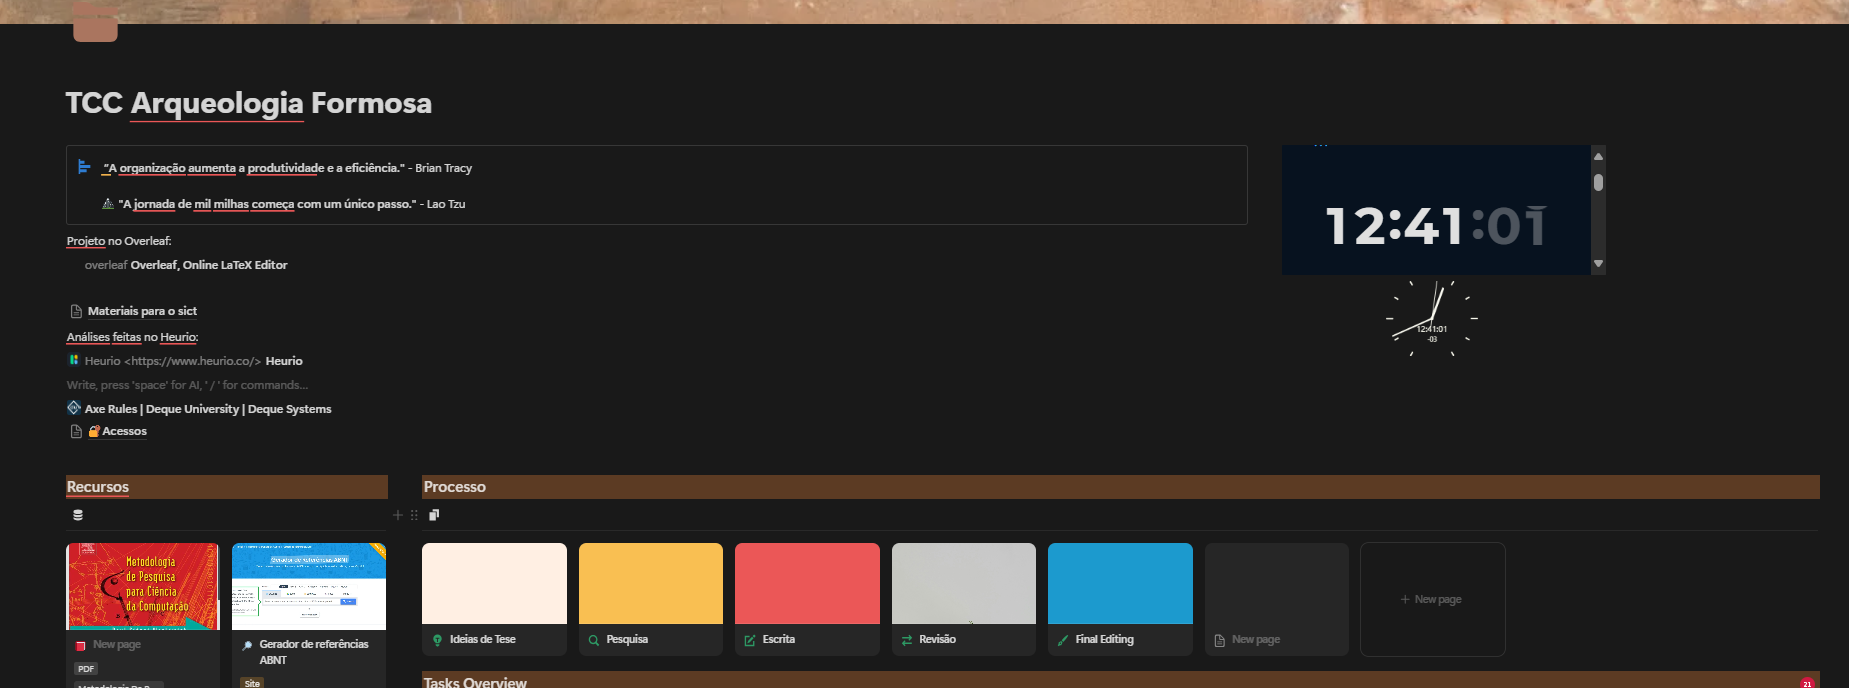
\includegraphics[height=6cm, keepaspectratio]{img/Notion/pagina inicial.png}
    \caption{ Página inicial do Notion para organização do TCC com etapas, \\ documentos úteis e ferramentas. \\
        \textbf{Fonte:} Elaborado pelo autor.}
    \label{fig:notion inicial}
\end{figure}

\begin{figure}[H]
    \centering
    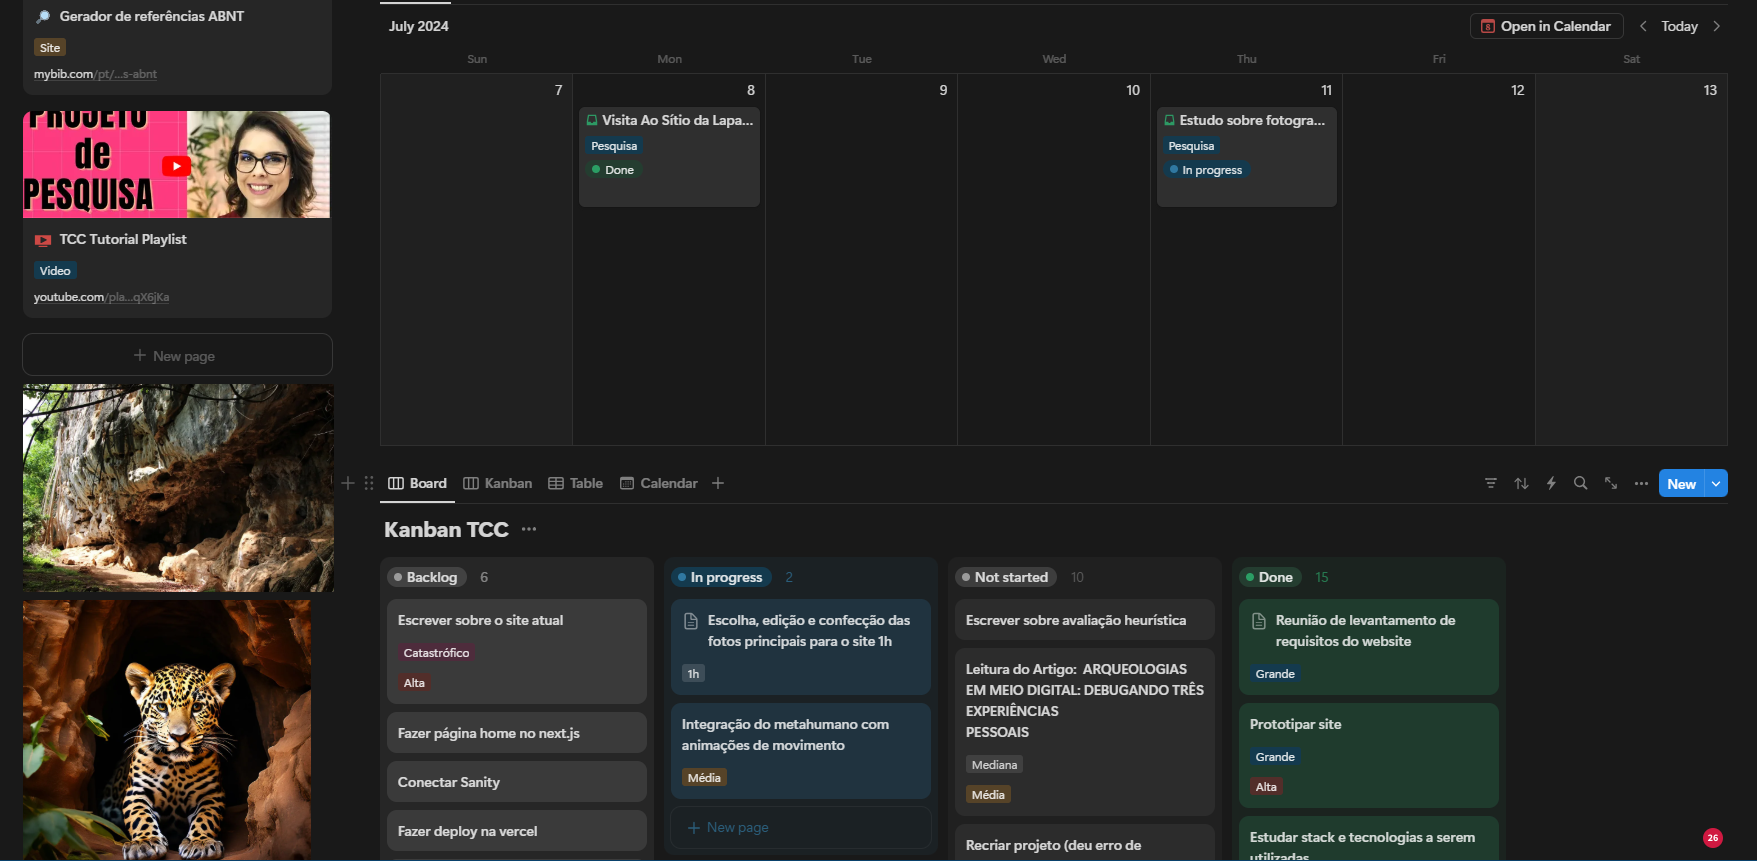
\includegraphics[height=8cm, keepaspectratio]{img/Notion/kanban.png}
    \caption{ Quadro Kanban e calendário para gerenciar atividades. \\
        \textbf{Fonte:} Elaborado pelo autor.}
    \label{fig:kanban notion}
\end{figure}


\subsection{Figma}
O Figma é uma ferramenta de design de interfaces baseada em nuvem, amplamente utilizada para criação de protótipos, designs colaborativos e sistemas de design. Ele se destaca por permitir que múltiplos usuários trabalhem simultaneamente em um mesmo projeto, facilitando a colaboração em tempo real. Além disso, o Figma oferece recursos como componentes reutilizáveis, autolayout e integração com outras ferramentas de desenvolvimento, tornando-o uma escolha popular entre designers e equipes de produto \citep{figma}.

% \subsection{Reality Capture}
% O \textbf{Reality Capture} é uma tecnologia de digitalização 3D que permite criar modelos tridimensionais altamente detalhados a partir de fotografias ou varreduras a laser. Essa ferramenta é amplamente utilizada em áreas como arquitetura, patrimônio cultural, produção cinematográfica e desenvolvimento de jogos, devido à sua capacidade de capturar objetos e ambientes reais com precisão e eficiência \citep{RealityCapture2023}.

% Uma das principais vantagens do Reality Capture é a sua precisão na reprodução de detalhes, o que o torna ideal para projetos que exigem fidelidade ao mundo real. Além disso, a tecnologia é eficiente, permitindo a digitalização de grandes estruturas ou objetos em um tempo relativamente curto. Os modelos gerados podem ser facilmente integrados a softwares de edição 3D e motores de jogos, como o Unreal Engine, o que amplia suas aplicações práticas \citep{RealityCapture2023}.

% No contexto de preservação do patrimônio cultural, o Reality Capture tem sido utilizado para digitalizar monumentos e sítios arqueológicos, garantindo que essas obras sejam preservadas digitalmente para futuras gerações. Na indústria de jogos e filmes, a ferramenta é empregada para criar assets 3D realistas, como personagens e cenários, que podem ser utilizados em produções de alta qualidade \citep{RealityCapture2023}.

% \subsection{Unreal Engine}
% A \textbf{Unreal Engine}, desenvolvida pela Epic Games, é um dos motores de jogo mais populares e versáteis do mercado. Conhecido por sua capacidade de renderizar gráficos de alta qualidade e suportar experiências interativas em tempo real, o Unreal Engine é amplamente utilizado não apenas no desenvolvimento de jogos, mas também em áreas como arquitetura, cinema e educação \citep{UnrealEngine2023}.

% Um dos recursos mais destacados do Unreal Engine é o sistema de \textit{Blueprints}, que permite a criação de lógica de jogo sem a necessidade de escrever código. Isso torna a ferramenta acessível para designers e artistas, que podem prototipar e desenvolver projetos de forma mais ágil. Além disso, o motor oferece suporte a tecnologias avançadas, como iluminação global e física realista, que contribuem para a criação de ambientes visualmente impressionantes \citep{UnrealEngine2023}.

% A integração do Unreal Engine com ferramentas como o Reality Capture é outro ponto forte. Modelos 3D gerados a partir de digitalizações do mundo real podem ser importados diretamente para o motor, onde podem ser manipulados e incorporados em projetos interativos. Essa combinação de tecnologias tem sido amplamente utilizada na criação de jogos realistas, simulações arquitetônicas e até mesmo em produções cinematográficas \citep{UnrealEngine2023}.

% Na área de educação, o Unreal Engine tem sido empregado para desenvolver simulações interativas e ambientes de aprendizagem imersivos. Sua flexibilidade e suporte a múltiplas plataformas, incluindo dispositivos móveis e realidade virtual, tornam-no uma escolha popular para projetos que exigem inovação e engajamento \citep{UnrealEngine2023}.

\subsection{Vercel}
A Vercel é uma plataforma de \gls{deploy} e hospedagem voltada para aplicações modernas, especialmente aquelas construídas com \glspl{framework} como Next.js, React e outros. Ela oferece integração contínua, escalabilidade automática e um desempenho otimizado para aplicações web estáticas e dinâmicas. Com foco na experiência do desenvolvedor, a Vercel simplifica o processo de publicação, permitindo que atualizações sejam feitas rapidamente através de integração com \gls{repositorio-git}. Sua infraestrutura global de \glsboth{cdn} garante baixa latência e alta disponibilidade para usuários finais \citep{vercel}.

\subsection{Heurio}
A extensão \textbf{Heurio} é uma ferramenta desenvolvida para auxiliar na realização de análises heurísticas de sites e interfaces digitais. Disponível como uma extensão para navegadores, o Heurio permite que profissionais de UX apliquem as heurísticas de usabilidade de forma prática e organizada, identificando problemas de usabilidade e propondo melhorias. \citep{Heurio}.

Dentre as funcionalidades do Heurio que facilitam a análise heurística estão:

\begin{itemize}
    \item \textbf{Lista de Heurísticas Integrada}: A extensão inclui uma lista de heurísticas de usabilidade, como as de Nielsen, que podem ser selecionadas e aplicadas diretamente durante a avaliação da interface.
    
    \item \textbf{Anotações e Comentários}: O Heurio permite que o avaliador faça anotações e comentários sobre problemas identificados, associando-os às heurísticas correspondentes. Isso facilita a documentação e a comunicação dos resultados.
    
    \item \textbf{Captura de Tela}: A ferramenta permite capturar telas da interface sendo avaliada, facilitando a visualização e a referência aos problemas encontrados.
    
    \item \textbf{Relatórios Automatizados}: Após a análise, o Heurio gera relatórios automatizados que organizam as anotações, capturas de tela e heurísticas aplicadas. Esses relatórios podem ser exportados e compartilhados com a equipe.
    
    \item \textbf{Colaboração em Equipe}: O Heurio suporta a colaboração entre múltiplos avaliadores, permitindo que equipes trabalhem juntas na mesma análise e compartilhem insights.
\end{itemize}

Essa ferramenta é particularmente útil em projetos de \textit{redesign} de sites, avaliação de protótipos e testes de usabilidade. Ela pode ser utilizada por equipes de \gls{ux}, designers e desenvolvedores para garantir que as interfaces atendam aos princípios de usabilidade e proporcionem uma experiência positiva ao usuário. Além disso, a ferramenta é flexível o suficiente para ser adaptada a diferentes contextos e metodologias de avaliação. \citep{Heurio}.

\subsection{Inno Setup}
O Inno Setup é um instalador gratuito para programas Windows, amplamente utilizado devido à sua facilidade de configuração e flexibilidade. Ele permite a criação de scripts de instalação personalizados, suportando recursos como criação de atalhos, registro de DLLs e desinstalação completa. Sua sintaxe é baseada em arquivos de texto no formato \texttt{.iss}, que são compilados para gerar executáveis de instalação. Por ser leve e de código aberto, o Inno Setup é uma escolha popular para desenvolvedores que buscam uma solução eficiente para distribuição de software \citep{innosetup}.
\chapter{Metodologia}
\label{cap:metodologia}

O presente trabalho adota a metodologia \gls{dsr}, conforme descrita por \cite{peffers2007design}, que propõe um modelo estruturado para a construção e avaliação de artefatos tecnológicos. A \gls{dsr} é amplamente utilizada em pesquisas de computação e engenharia de software, pois permite a criação de soluções inovadoras baseadas em problemas reais \citep{horita2019design}.

\section{Fases da Design Science Research}

\cite{peffers2007design} definem seis fases principais para a DSR:

\begin{enumerate}
    \item \textbf{Identificação do Problema e Motivação}: Definição do problema e justificativa de sua relevância.
    \item \textbf{Definição dos Objetivos da Solução}: Especificação do que a solução deve alcançar.
    \item \textbf{Design e Desenvolvimento}: Construção do artefato proposto dividida em ciclos.
    \item \textbf{Demonstração}: Aplicação da solução em um contexto real.
    \item \textbf{Avaliação}: Verificação da eficácia da solução.
    \item \textbf{Comunicação}: Divulgação dos resultados para a comunidade científica e profissionais da área.
\end{enumerate}

\section{Adaptação para Cinco Fases}

Neste trabalho, as fases da DSR foram adaptadas para um modelo de cinco etapas, de forma a organizar melhor o fluxo do projeto:

\begin{enumerate}
    \item \textbf{Identificação do Problema};
    \item \textbf{Definição dos Objetivos da Solução};
    \item \textbf{Design e Desenvolvimento};
    \item \textbf{Avaliação};
    \item \textbf{Comunicação}.
\end{enumerate}

Essa adaptação mantém a essência da DSR ao abranger a identificação do problema, definição dos objetivos, construção da solução, avaliação e comunicação dos resultados, garantindo uma abordagem estruturada e alinhada aos objetivos do projeto.

\section{Fase 1: Identificação do Problema}\label{definicao_do_problema}
As abordagens tradicionais de divulgação digital, baseadas em imagens estáticas e textos, limitam a interatividade e a imersão necessárias para explorar sítios arqueológicos. Essa falta de recursos modernos reduz o engajamento do público e dificulta a compreensão espacial desses patrimônios.
No caso do patrimônio arqueológico de Formosa, Goiás, o site original no Blogger desempenhou um papel importante na documentação inicial e na democratização do acesso a pesquisas sobre o Bisnau. No entanto, suas limitações técnicas, como baixa usabilidade, identidade visual desatualizada e restrições de personalização, comprometem a experiência do usuário e o alcance do conteúdo.
Para superar essas limitações, propôs-se o desenvolvimento de um Ambiente Virtual 3D, que permitirá uma exploração imersiva dos sítios arqueológicos e poderá ser baixado pelo novo site. A validação da proposta incluiu:

\begin{itemize}
\item \textbf{Visitas de campo}: Coleta de imagens e informações sobre os sítios, observando deteriorações como pichações e erosão.
\item \textbf{Análise Heurística}: Avaliação do site original com base nas 10 heurísticas de Nielsen, identificando falhas críticas como navegação confusa e falta de acessibilidade.
\end{itemize}

\subsection{Visitas de Campo}
As visitas de campo foram realizadas no sítio arqueológico da Lapa da Pedra, localizado na região nordeste de Formosa, Goiás. Conforme descrito no Referencial Teórico (\ref{sec:sitio lapa da pedra}), o sítio abriga 29 grutas, das quais sete contêm registros de arte rupestre. A Gruta IV S. = Gruta XIV M.–-47.302462,-15.493179 foi o foco principal deste trabalho, sendo a maior e a que contém mais desenhos.

Durante as visitas, observou-se que as pinturas estão distribuídas em alturas variáveis, desde 0,40 metros até 7,50 metros, em superfícies lisas, saliências e reentrâncias naturais do calcário. Apesar de sua relevância histórica, foram identificados sinais de deterioração tanto natural quanto antrópica. Entre os danos naturais, destacam-se a descamação da tinta, infiltrações e fissuras nas rochas, conforme discutido na seção sobre ameaças à preservação (\ref{sec:amecas a preservação}).

Quanto à ação humana, notou-se pichações e escritas superpostas às pinturas originais (Figura \ref{fig:degradacao vera}), reflexo da falta de conscientização sobre a importância cultural do sítio. Esses indícios reforçam a necessidade de estratégias de preservação digital e divulgação ampla, como discutido na Introdução.
\begin{figure}[H]
    \centering
    \includegraphics[height=8cm, keepaspectratio]{img/Visitas tecnicas/depredacao vera.JPG}
    \caption{Escritas superpostas à pinturas original. \\ Está escrito "Vera visitou em 28 de 10 de 62". \\
        \textbf{Fonte:} Elaborado pelo autor.}
    \label{fig:degradacao vera}
\end{figure}

Além disso, a localização do sítio em uma propriedade privada, a Fazenda Pedra, contribuiu para sua preservação parcial, mas também limita o acesso e a visibilidade do patrimônio para a população local. Essa constatação evidencia a urgência de iniciativas que promovam a democratização do acesso ao patrimônio cultural, alinhadas ao objetivo deste projeto.

\subsection{Análise Heurística do Antigo Site}
A análise heurística foi realizada no site antigo hospedado na plataforma Blogger com o auxílio da ferramenta Heurio, utilizando como referência as 10 heurísticas de usabilidade propostas por Jakob Nielsen (1994). A análise foi feita por quatro avaliadores: Naoki Rafael Miura, Victor Hugo Sales dos Reis, Sara Candido Fernandes e Erik Takeshi Miura, que identificaram problemas de usabilidade e navegabilidade.
A Figura \ref{fig:interface heurio} mostra a interface do Heurio, enquanto as Figuras \ref{fig:comentario heurio} e \ref{fig:fluxo} mostram o fluxo para inserir as observações da análise, que envolve a identificação do problema, a sugestão de melhoria e a indicação de qual heurística o problema está relacionado.
\begin{figure}[H]
    \centering
    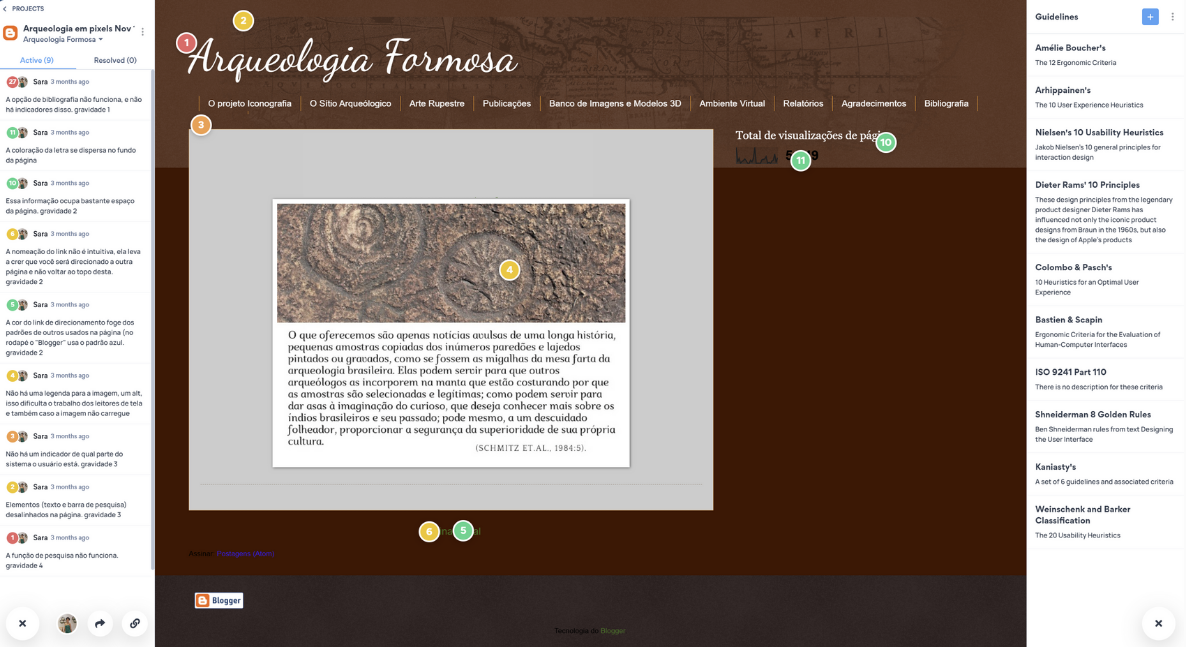
\includegraphics[height=8cm, keepaspectratio]{img/heurio/interface heurio.png}
    \caption{ Interface da ferramenta Heurio. Ela exibe o site a ser analisado, \\ os comentários já feitos no lado esquerdo e os grupos de heurísticas do lado direito. \\
        \textbf{Fonte:} Elaborado pelo autor.}
    \label{fig:interface heurio}
\end{figure}

\begin{figure}[H]
    \centering
    \begin{minipage}[b]{0.48\textwidth}
        \centering
        \includegraphics[height=6cm, keepaspectratio]{img/heurio/habilitar comentários.png}
        \caption{Botão de habilitar comentários no Heurio.  \\
            \textbf{Fonte:} Elaborado pelo autor.}
        \label{fig:comentario heurio}
    \end{minipage}
    \hfill
    \begin{minipage}[b]{0.48\textwidth}
        \centering
        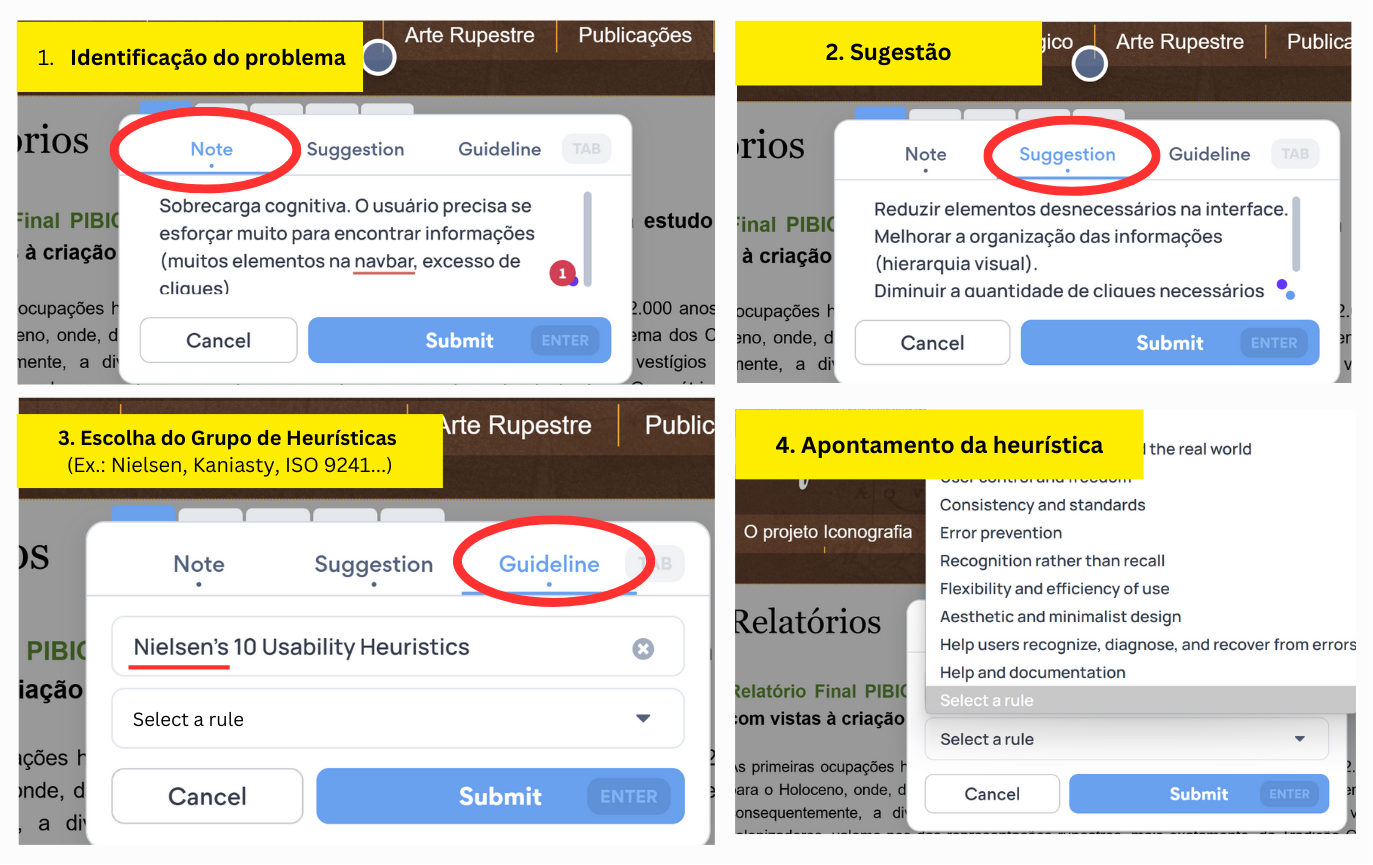
\includegraphics[height=6cm, keepaspectratio]{img/heurio/fluxo heurio.png}
        \caption{Fluxo de observações incluindo identificação \\do problema, sugestão e heurística relacionada. \\
            \textbf{Fonte:} Elaborado pelo autor.}
        \label{fig:fluxo heurio}
    \end{minipage}
\end{figure}

Por fim, a ferramenta Heurio gera um quadro para visualização como se fosse um relatório (Figura \ref{fig:quadro resultados}). Essas observações de cada um dos analistas foram reunidas e contribuíram para a identificação do problema, possibilitando a melhoria do site. 
\begin{figure}[H]
    \centering
    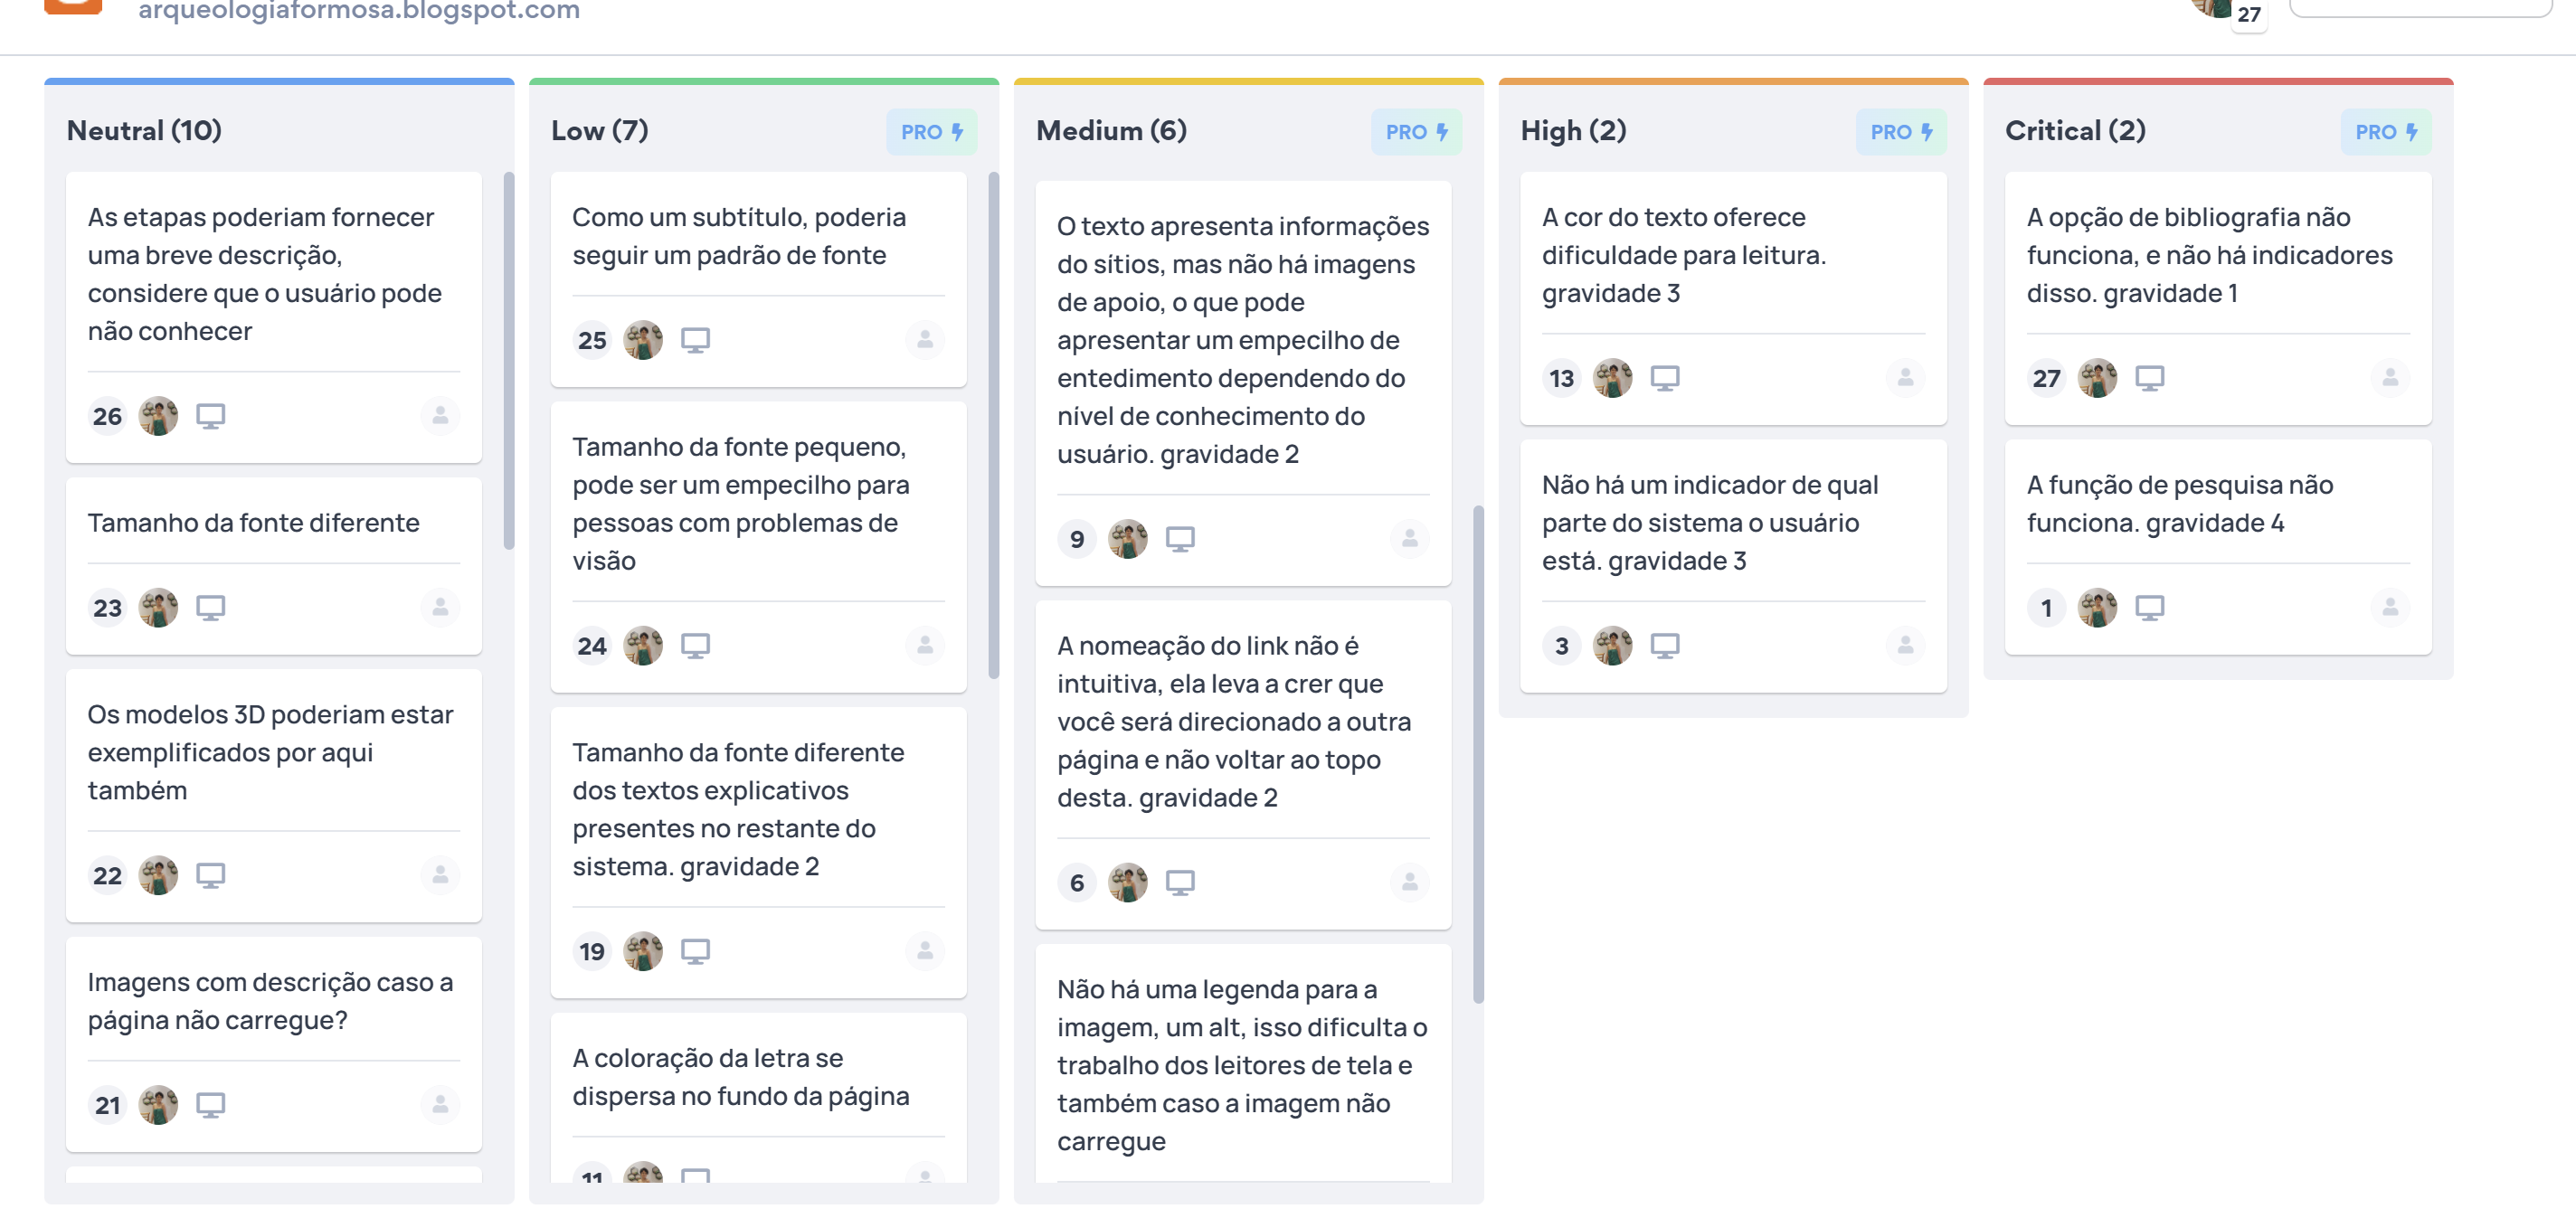
\includegraphics[height=8cm, keepaspectratio]{img/heurio/quadro resultados.png}
    \caption{ Quadro de resultados gerado após a análise do Heurio. \\
        \textbf{Fonte:} Elaborado pelo autor.}
    \label{fig:quadro resultados}
\end{figure}


\section{Fase 2: Definição dos Objetivos da Solução}\label{definicao_dos_objetivos_da_solucao}
Essa fase envolve a especificação do que a solução deve alcançar. Para isso foi utilizada a técnica de engenharia de requisitos.
\subsection{Coleta de Requisitos}
Coleta de requisitos foi realizada por meio de questionário online e entrevistas formais e informais com professores do IFG, resultando em 13 requisitos funcionais (Apêndice \ref{ap:requisitos-site-table}) e 13 não funcionais (Apêndice \ref{ap:requisitos-nao-funcionais-site-table}) para o site. Para o ambiente virtual há quatro requisitos funcionais (Apêndice \ref{ap:requisitos-ambiente-table}) e 2 requisitos não funcionais (Apêndice \ref{ap:requisitos-nao-funcionais-ambiente}). Todos os requisitos podem ser consultados no apêndice. 

\subsubsection{Identificação dos Requisitos}
\label{sec:identificacao_requisitos}

Por convenção e para facilitar a identificação dos casos de uso junto aos contextos, a referência é feita de acordo com o esquema abaixo:

\textbf{Sigla de subseção | numeração}

Os requisitos são identificados por uma sigla que representa a subseção (por exemplo, "RFS" para Requisitos Funcionais do site, “RNFA” para Requisitos Não Funcionais do Ambiente Virtual) seguida de um número sequencial.

\subsubsection{Prioridades dos Requisitos}
\label{sec:prioridades_requisitos}

Para estabelecer a prioridade dos requisitos, foram adotadas as denominações: essencial, importante e desejável. Abaixo temos a descrição de significado de cada uma dessas denominações:

\begin{table}[H]
\centering
\caption{Prioridades dos Requisitos}
\label{tab:prioridades_requisitos}
\begin{tabular}{|l|p{10cm}|}
\hline
\textbf{Prioridade} & \textbf{Descrição} \\ \hline
Essencial & Requisito sem o qual o sistema não entra em funcionamento. \\ \hline
Importante & Requisito que, sem ele, o sistema entra em funcionamento, mas de forma não satisfatória. \\ \hline
Desejável & Requisito que pode ser deixado para versões futuras sem comprometer as funcionalidades básicas. \\ \hline
\end{tabular}
\end{table}

\subsubsection{Requisitos Documentados}
\label{sec:requisitos_documentados}
{\small 
\begin{longtable}{|p{2.5cm}|p{4cm}|p{6cm}|p{2cm}|}
\caption{Exemplo da Tabela de Requisitos gerada}
\label{table:exemplo_tabela_requisitos} \\
\hline
\textbf{Identificador} & \textbf{Nome} & \textbf{Descrição} & \textbf{Prioridade} \\
\hline
\endfirsthead
\hline
\textbf{Identificador} & \textbf{Nome} & \textbf{Descrição} & \textbf{Prioridade} \\
\hline
\endhead
RFS001 & Exemplo de Nome & Exemplo de descrição do requisito & Essencial, Importante ou Desejável \\ \hline
\end{longtable}
}
Para acessar os requisitos gerados na íntegra, consulte os Apêndices \ref{apendice} e \ref{Apendice B}.


\section{Fase 3: Design e Desenvolvimento}\label{sec: Fase 3 design e desenvolvimento}
Após a identificação do problema \ref{definicao_do_problema} e a definição dos objetivos \ref{definicao_dos_objetivos_da_solucao} da solução, esta seção descreve o processo de design e desenvolvimento do projeto. Seguindo a abordagem da \gls{dsr}, conforme descrita por \cite{peffers2007design}, o desenvolvimento foi estruturado em ciclos iterativos, permitindo refinamento contínuo dos artefatos conforme novas descobertas e avaliações eram feitas.
Neste projeto, os ciclos foram organizados de forma a contemplar as principais etapas do desenvolvimento da solução:

% Ciclo 1
\subsection*{Ciclo 1: Fotogrametria e Construção do Modelo 3D} \label{subsec:ciclo1}

\subsubsection*{Objetivo do Ciclo}
Criar um modelo 3D detalhado baseado em imagens capturadas em campo. Atender ao RFA001 (Modelo 3D de Alta Qualidade) e garantir compatibilidade com Unreal Engine 5.4. 

\subsubsection*{Ações Realizadas}
\begin{enumerate}
    \item Captura de imagens de alta resolução de diferentes ângulos do sítio da Lapa da Pedra e seleção para remover fotos com ruídos.
    \item Processamento no Reality Capture para reconstrução fotogramétrica, resultando em um modelo inicial com 102 milhões de polígonos.
    \item Simplificação do modelo para 5 milhões de polígonos, garantindo compatibilidade com a Unreal Engine (RFA001).
    \item Reprojeção de textura do modelo de alta resolução para o modelo simplificado, mantendo a qualidade visual.
\end{enumerate}

\textbf{Resultado}: Modelo 3D detalhado e otimizado para uso no ambiente virtual, garantindo fidelidade visual e desempenho adequado na Unreal Engine 5.4 (RFA001).

% Ciclo 2
\subsection*{Ciclo 2: Construção do Ambiente Virtual na Unreal Engine 5.4} \label{subsec:ciclo2}

\subsubsection*{Objetivo do Ciclo}
Atender aos requisitos RFA002 (Navegação em Terceira Pessoa), RFA003 (Alternância de Câmera), RFA004 (Avatar Personalizado), RNFA001 (Compatibilidade com Windows), RNFA002 (Documentação de Instalação) e RNFA003 (Instalação Simplificada).

\subsubsection*{Ações Realizadas}
\begin{enumerate}
    \item Importação do modelo 3D otimizado na Unreal Engine 5.4.
    \item Criação do cenário virtual com texturas realistas e iluminação dinâmica.
    \item Implementação do sistema de navegação em terceira pessoa com controle de um avatar interativo (RFA002).
    \item Criação de um avatar personalizado no Metahuman com aparência semelhante ao professor Edson Borges (RFA004).
    \item Desenvolvimento de um sistema de alternância de câmera, permitindo troca entre visão em primeira e terceira pessoa (RFA003).
    \item Configuração de otimizações gráficas para garantir um bom desempenho em máquinas com Windows 10 ou superior (RNFA001).
    \item Empacotamento do ambiente virtual em um arquivo executável (.exe) para distribuição, garantindo instalação simplificada para usuários finais (RNFA003).
    \item Desenvolvimento de um guia de instalação e configuração para orientar os usuários na utilização do ambiente virtual (RNFA002).
\end{enumerate}

\textbf{Resultado}: Ambiente virtual interativo e otimizado, permitindo exploração em terceira pessoa com opção de alternância para visão em primeira pessoa, avatar personalizado, compatibilidade com Windows 10+ e um instalador simplificado para facilitar a distribuição e configuração pelos usuários finais (RFA002, RFA003, RFA004, RNFA001, RNFA002, RNFA003).

% Ciclo 3
\subsection*{Ciclo 3: Prototipação do Novo Site} \label{subsec:ciclo3}

\textbf{Objetivo do Ciclo}: Desenvolver um protótipo o novo site, atendendo aos requisitos funcionais RFS002 (Exibir Galeria de Imagens), RFS006 (Buscar Trabalhos por Filtros) e RFS007 (Informações de Contato), bem como aos requisitos não funcionais RNFS006 (Acessibilidade), RNFS008 (Responsividade) e RNFS012 (SEO).

\subsection{Ações Realizadas}
\begin{enumerate}
    \item Análise das referências e inspirações enviadas pelo professor Edson Borges por meio de um questionário.
    \item Reorganização da arquitetura da informação, agrupando conteúdos relevantes e reduzindo cliques (RNFS006).
    \item Criação de wireframes para estruturar a interface e definir a disposição dos elementos visuais (RNFS008).
    % \item Definição da paleta de cores e tipografia, garantindo coerência visual e acessibilidade (RNFS006).
    \item Criação de uma nova logo, inspirada nas cores das artes rupestres da Lapa da Pedra.
    \item Desenvolvimento de um protótipo de alta fidelidade no Figma, representando a versão final do site.
    \item Validação e refinamento do protótipo a partir de feedbacks coletados com o professor e colegas.
    \item Organização eficiente do projeto no Figma, facilitando futuras iterações e implementações.
\end{enumerate}

\textbf{Resultado}: Protótipo de alta fidelidade bem estruturado e validado, garantindo acessibilidade, melhor navegação, identidade visual consistente e um layout flexível para futuras alterações e desenvolvimento (RNFS006, RNFS008, RNFS014).
% 4
\subsection*{Ciclo 4: Desenvolvimento do Novo Site} \label{subsec:ciclo4}

\subsubsection*{Objetivo do Ciclo}
Atender aos requisitos funcionais e não funcionais do site. O desenvolvimento abrange a maioria dos requisitos especificados nas tabelas \ref{ap:requisitos-site-table} e \ref{ap:requisitos-nao-funcionais-site-table}, garantindo acessibilidade, responsividade, gerenciamento dinâmico de conteúdo e otimização de desempenho.

\subsubsection*{Ações Realizadas}
\begin{enumerate}
\item \textbf{Configuração do ambiente de desenvolvimento}: Definição da arquitetura \textit{JAMstack}, utilizando o \textit{framework} \textit{Next.js} e a biblioteca \textit{Schema UI} no \textit{frontend} e \textit{Sanity} como CMS headless, além da configuração do repositório no Git e escolha da hospedagem na Vercel para otimização de desempenho e redução de custos (RNFS001, RNFS008, RNFS011).

    
    \item \textbf{Implementação da estrutura e funcionalidades do site}
    \begin{enumerate}
        \item Implementação de páginas-chave:
        \begin{enumerate}
            \item Página inicial com navegação hierárquica
            \item Seções específicas para sítios arqueológicos
            \item Página de Contato
            \item Página de trabalhos escritos com filtros
        \end{enumerate}
    \end{enumerate}
    
\end{enumerate}

\section{Fase 4: Avaliação} \label{sec:avaliacao-dsr}

    \textbf{Validação Técnica}
    \begin{enumerate}
        \item Testes de performance com Lighthouse;
        \item Verificação de compatibilidade em 6 navegadores diferentes;
        \item Avaliação heurística do novo site e \textit{feedbacks}.
    \end{enumerate}
    

\section{Fase 5: Comunicação} \label{sec:comunicacao-dsr}

Os resultados foram divulgados através de:
\begin{itemize}
    \item \textbf{Documentação Acadêmica}: Este TCC;
    \item \textbf{Publicação Online}: Site em \url{https://arqueologiaformosa.com.br}.
\end{itemize}



\chapter{Desenvolvimento}
\label{cap:desenvolvimento}

Nesta seção, detalha-se o processo de desenvolvimento do projeto, abrangendo todas as etapas desde a concepção inicial até a implementação final utilizando os ciclos de desenvolvimento da metodologia DSR descritas na Seção \ref{sec: Fase 3 design e desenvolvimento} do capítulo de Metodologia. São apresentados os métodos, ferramentas e tecnologias utilizadas, além dos desafios enfrentados e as soluções adotadas.


\section{Ciclo 1: Fotogrametria e Construção do Modelo 3D}
\label{sec:ciclo1_fotogrametria}

\textbf{Objetivo}: Criar um modelo 3D detalhado baseado em imagens capturadas em campo. Atender ao RFA001 (Modelo 3D de Alta Qualidade) e garantir compatibilidade com Unreal Engine 5.4. 

A seguir o processo é descrito detalhadamente.
    \subsection{Visitas de campo e Captura de Imagens} 
    Ao todo foram realizadas 3 visitas ao local de estudo, a Lapa da Pedra. 
    As primeiras visitas de campo, guiadas pelo Guia Ambiental e Condutor Cultural Noel José dos Santos, foram para estudo e planejamento da captura das imagens. O objetivo era analisar o terreno, identificar os pontos de interesse (pictoglifos e estrutura da gruta), e definir a melhor estratégia para a captura das imagens.

    Com a localização definida, e com a colaboração do professor Dr. Leomar Rufino Alves Júnior, especialista em fotogrametria, topografia, geodésia e sensoriamento remoto, deu-se início à etapa de aquisição de dados. Um veículo aéreo não tripulado (VANT) modelo Phantom 4 Standard (Figura \ref{fig:phantom 4}), equipado com câmera de alta resolução, foi utilizado para capturar imagens aéreas (Figuras \ref{fig:drone voando} e \ref{fig:drone dentro da caverna}) com superposição de pelo menos 70\% (Figura \ref{fig:fotos tiradas}, garantindo a cobertura completa da área e a precisão do modelo 3D. Simultaneamente, imagens terrestres foram coletadas com câmeras de celular e câmera fotográfica DSLR semi-profissional modelo Lumix Fz80 Panasoni, focando em detalhes específicos dos pictoglifos e da estrutura da gruta, principalmente os que estavam no teto - àrea que o drone não conseguia pegar com detalhes.

\begin{figure}[H]
    \centering
    % Primeira figura
    \begin{minipage}{0.45\textwidth} % Reduzi a largura para 45%
        \centering
    \includegraphics[height=8cm, keepaspectratio]{img/Visitas tecnicas/phantom 4.png}
    \caption{ Drone modelo Phantom 4, utilizado \\ para as capturas das imagens.\\
        \textbf{Fonte:} Acervo pessoal do Ramon Almeida.}
    \label{fig:phantom 4}   
    \end{minipage}
    \hspace{1cm} % Espaço fixo de 0.5cm entre as figuras
    % Segunda figura
    \begin{minipage}{0.45\textwidth} % Reduzi a largura para 45%
        \centering
        \includegraphics[height=8cm, keepaspectratio]{img/Visitas tecnicas/drone voando.png}
        \caption{Processo de captura de imagens com o \\ drone no exterior da caverna.\\
            \textbf{Fonte:} Acervo pessoal do professor Edson Borges.}
        \label{fig:drone voando}
    \end{minipage}
\end{figure}

\begin{figure}[H]
    \centering
        \includegraphics[height=8cm, keepaspectratio]{img/Visitas tecnicas/drone dentro da caverna.jpg}
        \caption{Processo de captura de imagens com o drone \\
        no interior da caverna. \\
            \textbf{Fonte:} Acervo pessoal do Ramon Almeida.}
        \label{fig:drone dentro da caverna}
\end{figure}

 Ao todo foram capturadas 1.493 imagens cobrindo diferentes ângulos do sítio arqueológico. Dessas fotos, 1018 foram selecionadas e as outras foram removidas por conter ruídos, desfoque ou má qualidade que poderiam atrapalhar o processo seguinte (Figura \ref{fig:fotos tiradas}).

\begin{figure}[H]
    \centering
    \includegraphics[height=8cm, keepaspectratio]{img/reality e fotogrametria processo/imagens capturas.png}
    \caption{Fotografias capturadas com superposição de 70\%.\\
        \textbf{Fonte:} Elaborado pelo autor.}
    \label{fig:fotos tiradas}   
\end{figure}

    \subsection{Processamento no Reality Capture para reconstrução fotogramétrica}
    \begin{enumerate}
\item \textbf{Alinhamento das Fotos} \\
Com as fotos devidamente selecionadas pôde-se seguir para a etapa de alinhamento, que ocorre no software Reality Capture. O software identifica pontos correspondentes nas imagens e calcula suas posições espaciais relativas (Figura \ref{fig:alinhamento}). Este processo resulta na criação de uma nuvem de pontos esparsa, que representa os principais elementos da cena. 
A partir da nuvem de pontos esparsa, o software gera uma nuvem de pontos densa (Figura \ref{fig:nuvem de pontos}), que contém uma quantidade significativamente maior de pontos e oferece maior detalhamento. Esta etapa é computacionalmente intensiva e depende da qualidade das imagens de entrada.

\begin{figure}[H]
    \centering
        \centering
        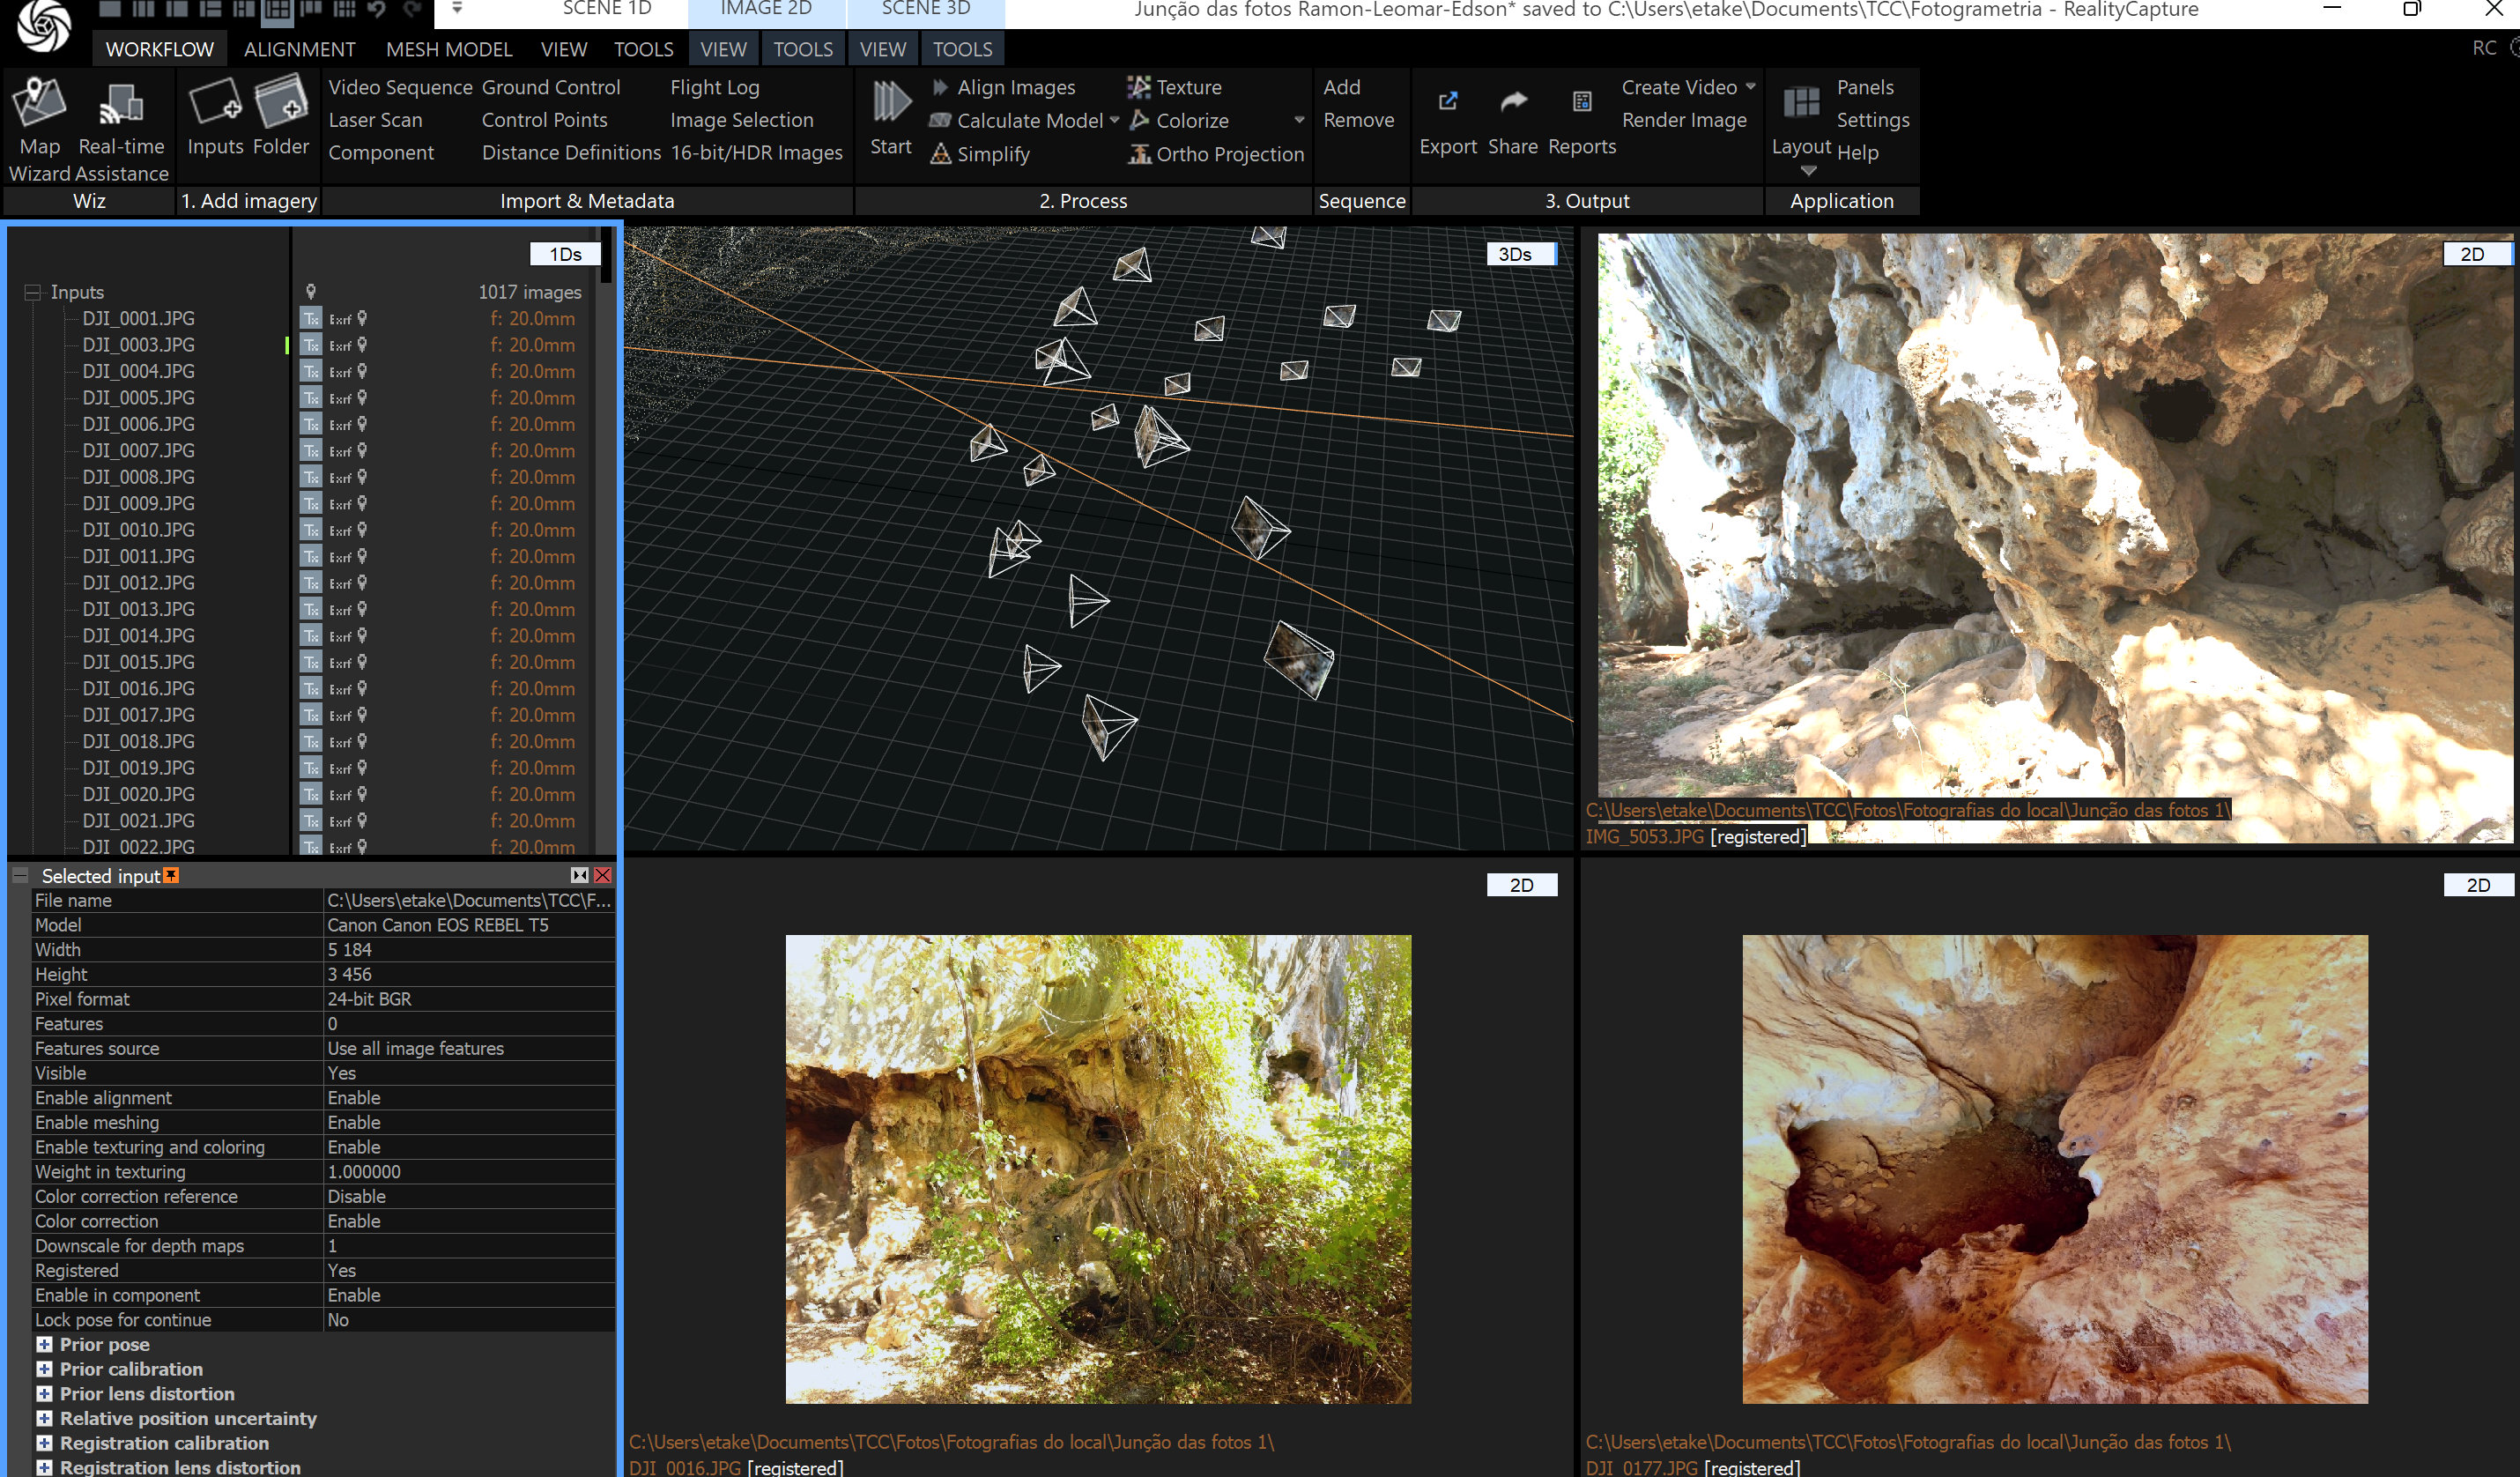
\includegraphics[height=8cm, keepaspectratio]{img/reality e fotogrametria processo/cameras alinhamento.png}
        \caption{Alinhamento das imagens pelo software Reality Capture. \\
            \textbf{Fonte:} Elaborado pelo autor.}
        \label{fig:alinhamento}
\end{figure}

\begin{figure}[H]
        \centering
        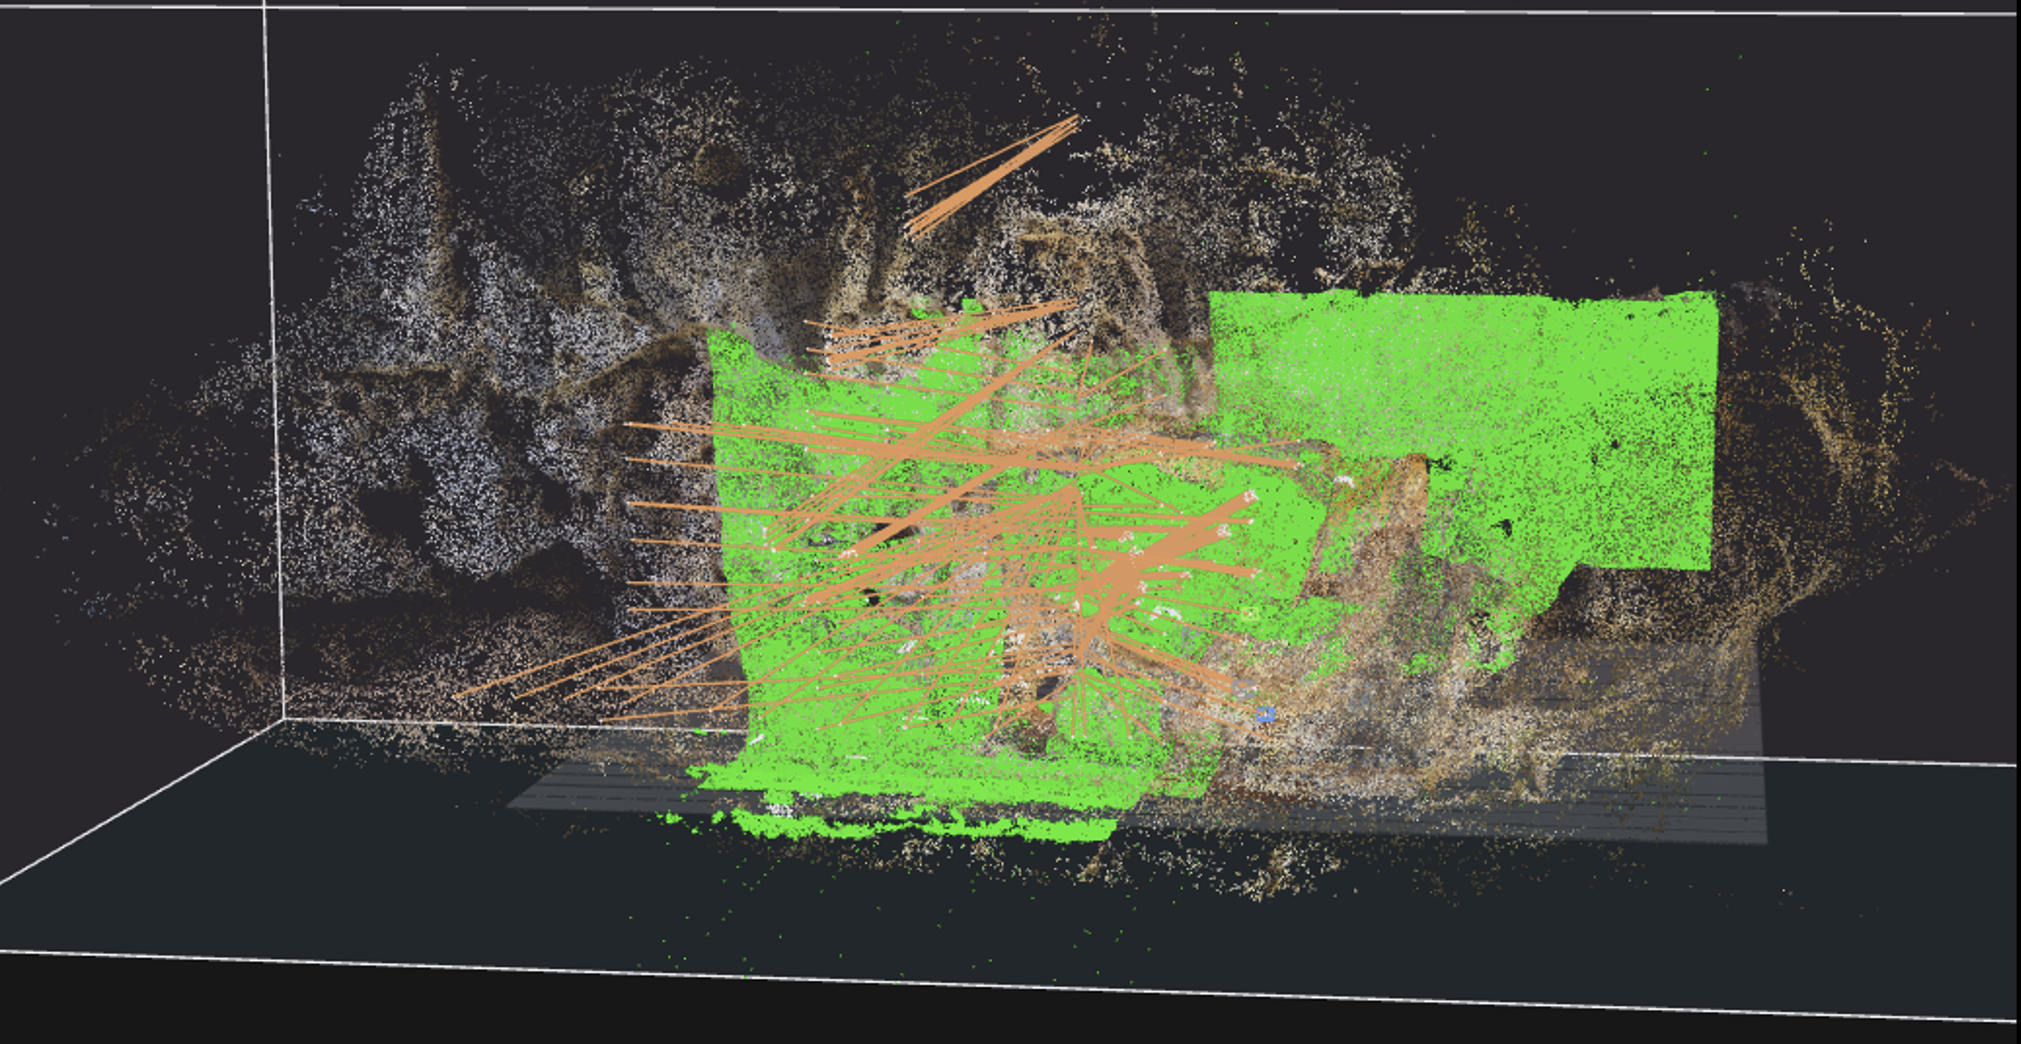
\includegraphics[height=8cm, keepaspectratio]{img/reality e fotogrametria processo/primeiro modelo componente.png}
        \caption{Nuvem de pontos densa. \\
            \textbf{Fonte:} Elaborado pelo autor.}
        \label{fig:nuvem de pontos}
\end{figure}


\item \textbf{Filtragem e Recorte} \\
Para eliminar pontos indesejados, como vegetação ou objetos móveis, foi realizada uma filtragem manual iterativa. Esta etapa é essencial para garantir que apenas os elementos relevantes sejam incluídos no modelo final.
\begin{figure}[H]
        \centering
        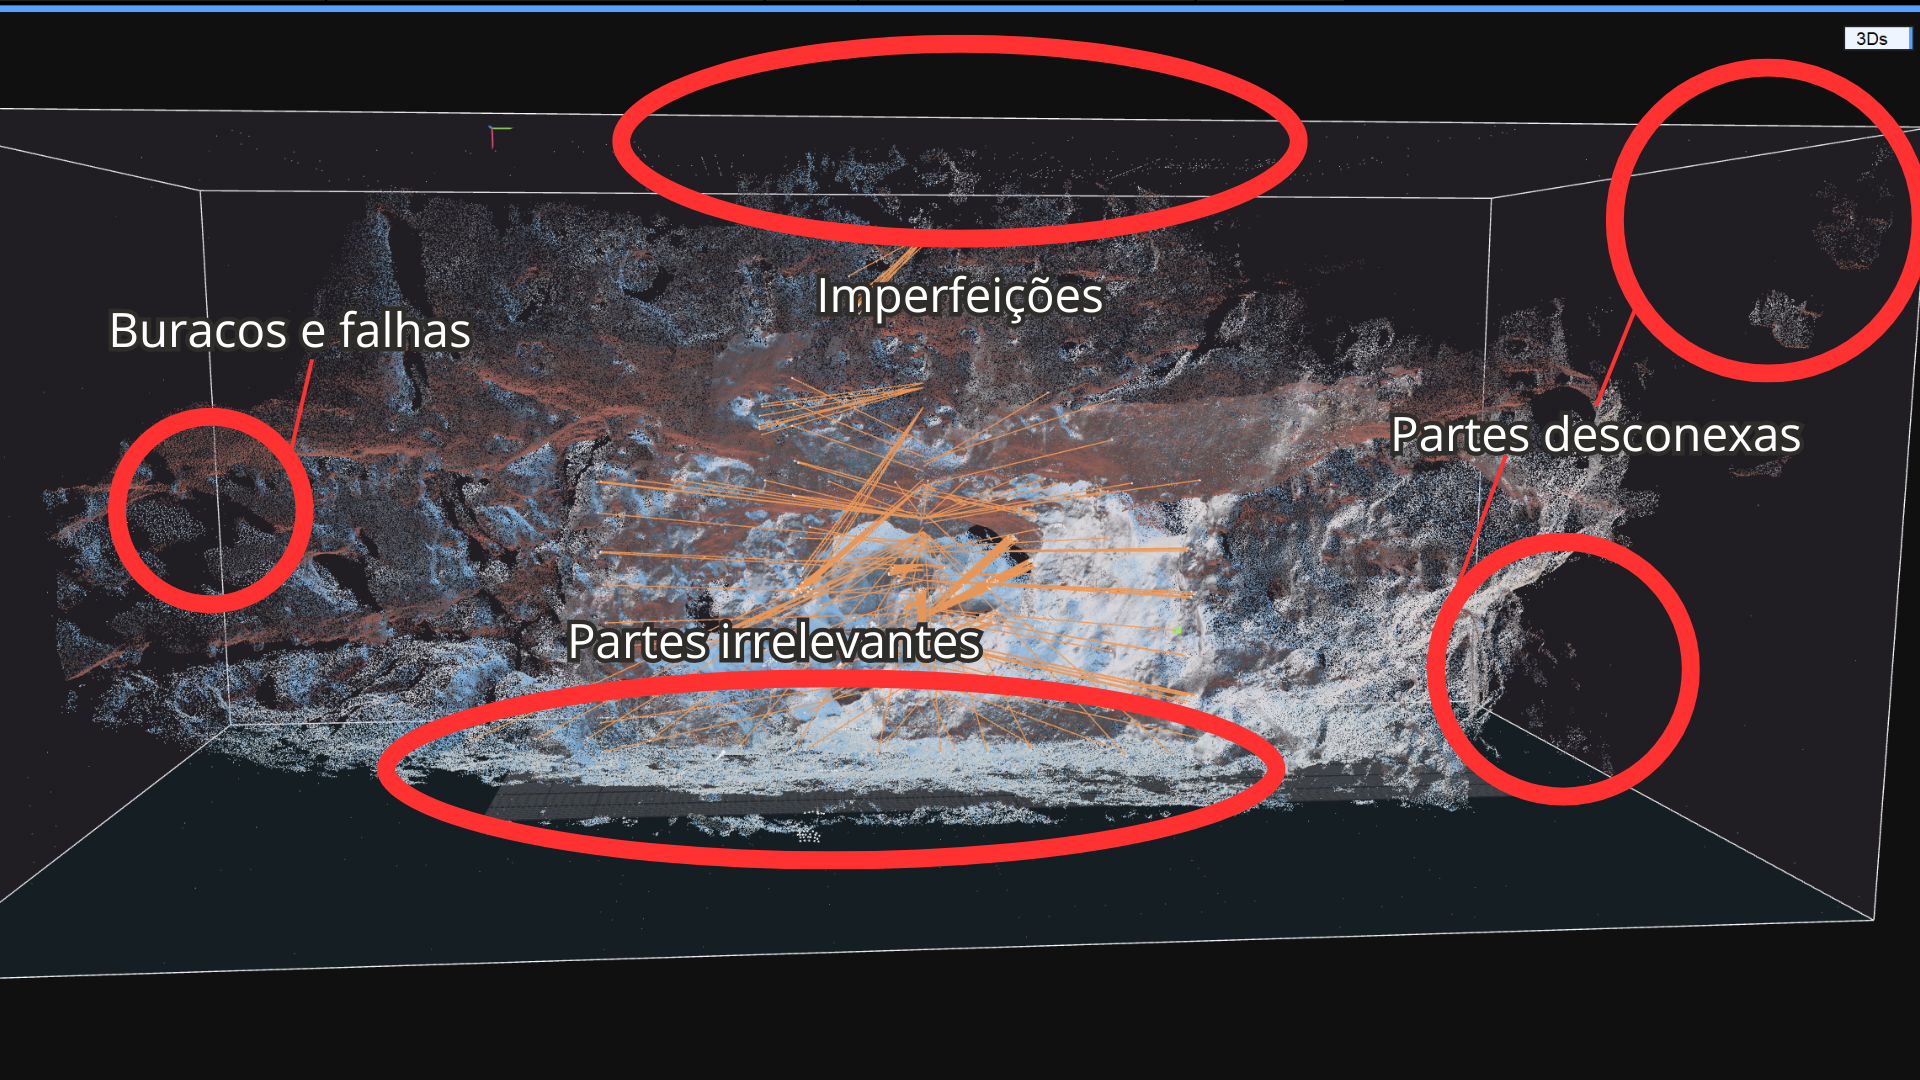
\includegraphics[height=8cm, keepaspectratio]{img/reality e fotogrametria processo/Criação de nuvem de pontos.png}
        \caption{Identificação dos pontos indesejados para filtragem. \\
            \textbf{Fonte:} Elaborado pelo autor.}
        \label{fig:filtragem}
\end{figure}

\item \textbf{Criação do Modelo 3D} \\
Com base na nuvem de pontos densa filtrada, o software gerou a malha poligonal do modelo 3D, como mostra a Figura \ref{fig:modelo 3D solido}. O modelo inicial continha 102 milhões de polígonos, resultando em um nível de detalhe extremamente alto, mas também em um arquivo muito pesado.
\begin{figure}[H]
        \centering
        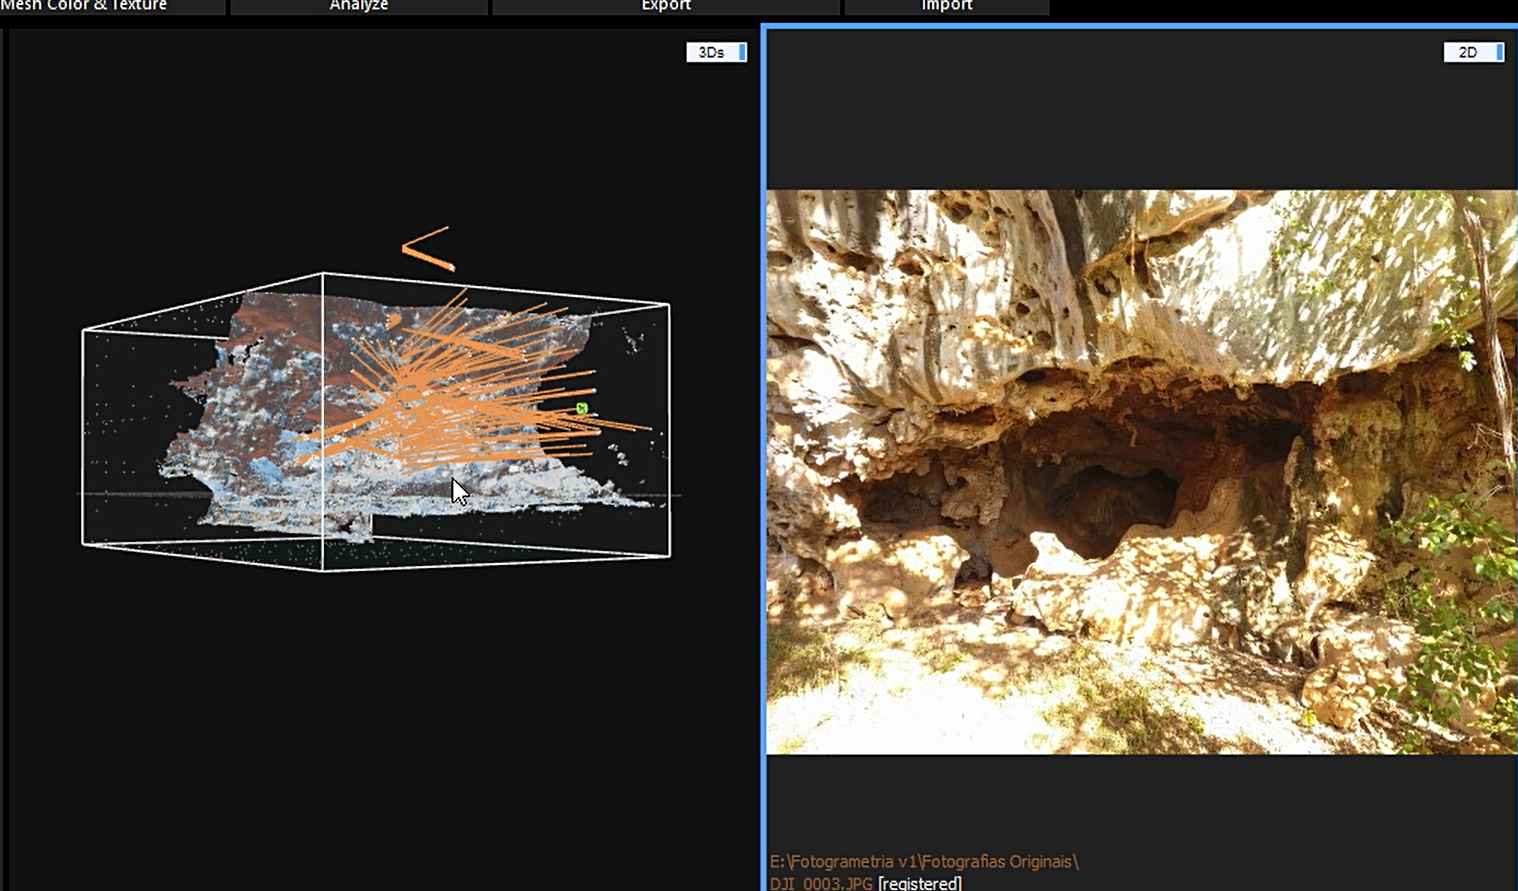
\includegraphics[height=8cm, keepaspectratio]{img/reality e fotogrametria processo/modelo solido e foto.png}
        \caption{Identificação dos pontos indesejados para filtragem. \\
            \textbf{Fonte:} Elaborado pelo autor.}
        \label{fig:modelo 3D solido}
\end{figure}

\item \textbf{Texturização} \\
O processo de texturização atribuiu cores e detalhes visuais à malha poligonal, utilizando informações das imagens originais. A textura gerada foi de alta qualidade, refletindo fielmente as características do ambiente capturado (Figura \ref{fig:texturizado}). Com esse modelo as figuras pré-históricas no interior da gruta ficaram nítidas e altamente visíveis, como mostra a Figura \ref{fig:interior}.

\begin{figure}[H]
        \centering
        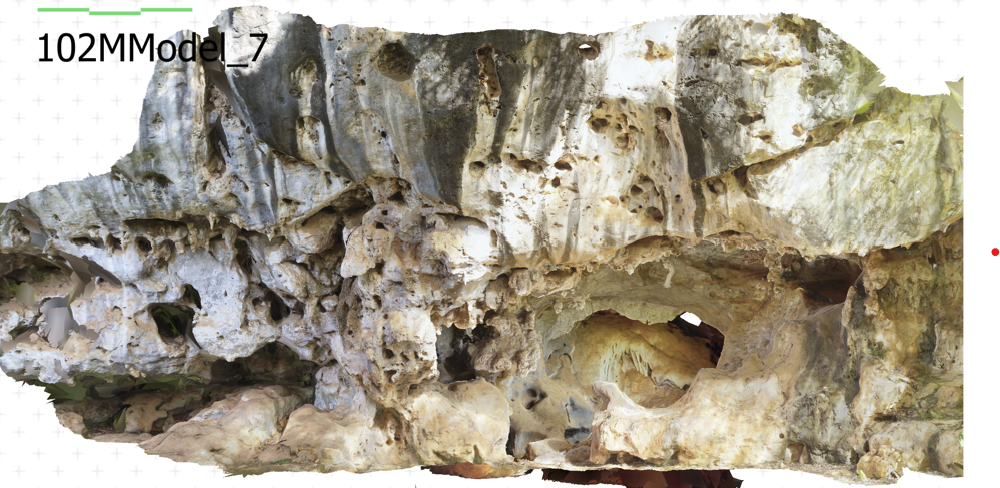
\includegraphics[height=8cm, keepaspectratio]{img/reality e fotogrametria processo/102M textura.png}
        \caption{Modelo texturizado de alta qualidade com 102 milhões de polígonos, parte exterior. \\
            \textbf{Fonte:} Elaborado pelo autor.}
        \label{fig:texturizado}
\end{figure}
\begin{figure}[H]
        \centering
        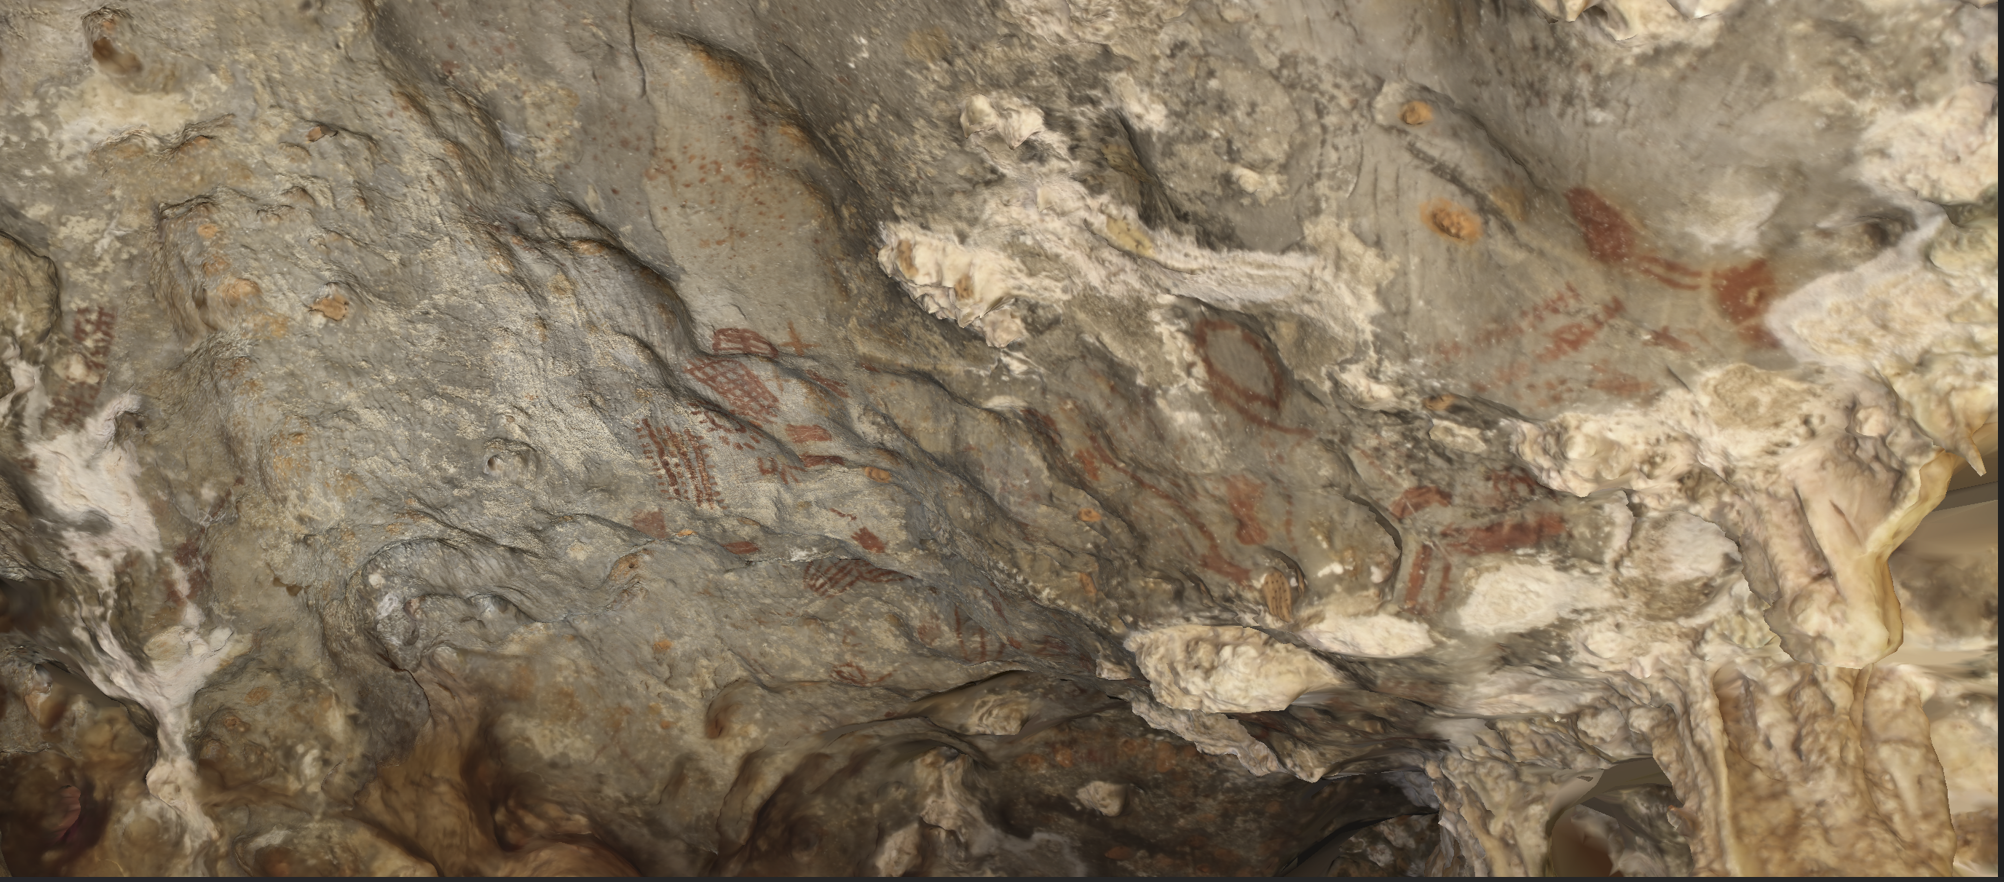
\includegraphics[height=8cm, keepaspectratio]{img/reality e fotogrametria processo/interior.png}
        \caption{Modelo texturizado de alta qualidade com 102 milhões de polígonos, parte interior. \\
            \textbf{Fonte:} Elaborado pelo autor.}
        \label{fig:interior}
\end{figure}
\end{enumerate}
    \section{Simplificação do Modelo 3D, garantindo compatibilidade com a Unreal Engine (RFA001).}
  
Devido ao tamanho do modelo inicial (102 milhões de polígonos), foi necessário realizar um processo de simplificação para torná-lo mais leve e compatível para uso em softwares como a Unreal Engine, que suporta bem até 5 milhões de polígonos. A malha foi reduzida consideravelmente tornando-o mais leve, porém a qualidade ficou muito ruim deixando os desenhos praticamete apagados, como mostra a Figura \ref{fig:modelo ruim}

\begin{figure}[H]
    \centering
    % Primeira figura
    \begin{minipage}{0.45\textwidth} % Reduzi a largura para 45%
        \centering
        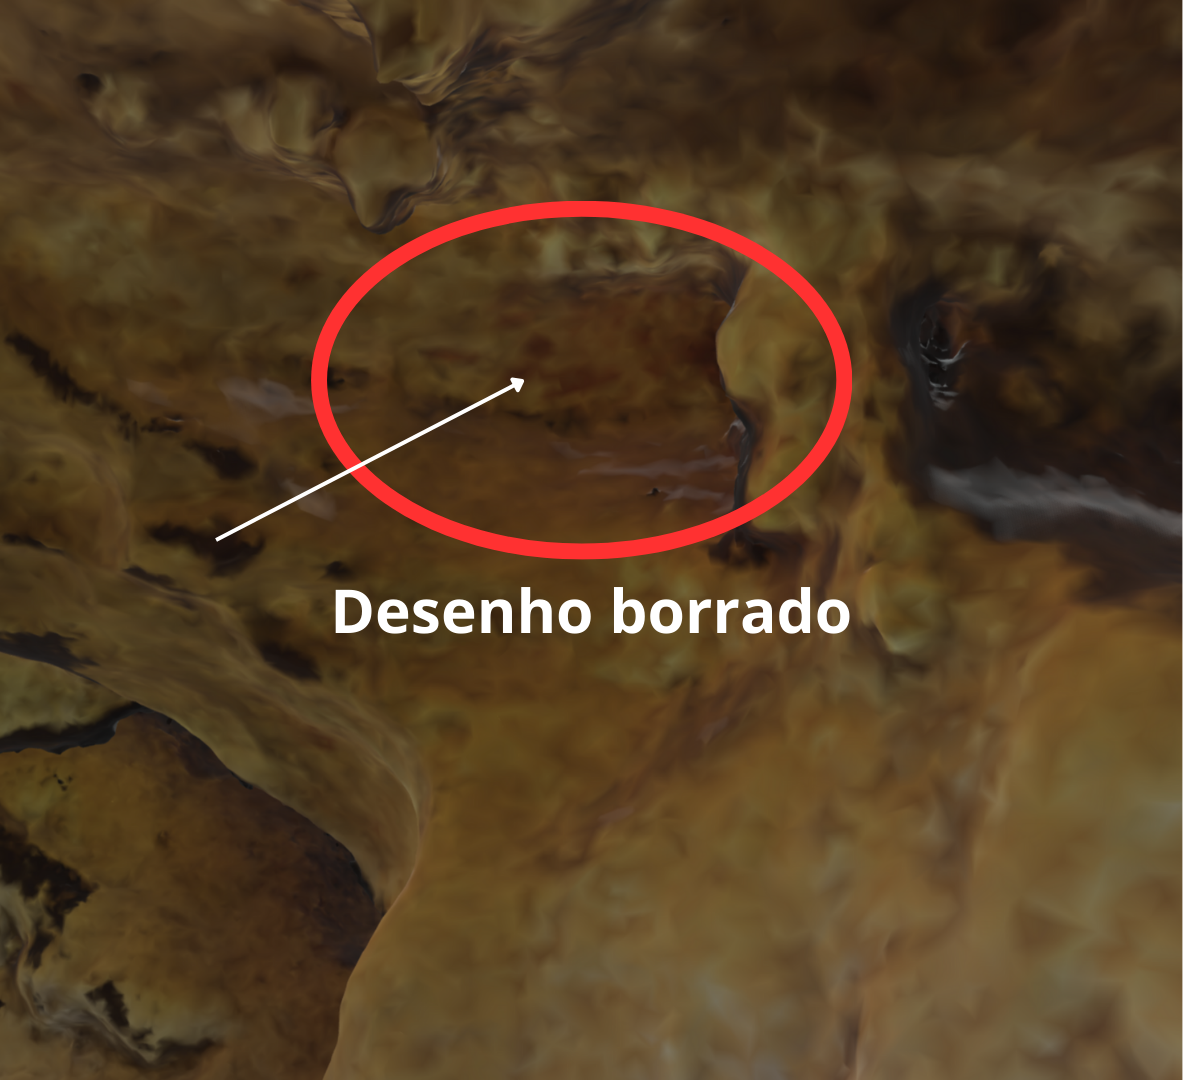
\includegraphics[height=5cm, keepaspectratio]{img/reality e fotogrametria processo/modelo ruim.png}
        \caption{Modelo simplificado com 5 milhões \\ de polígonos. Desenho apagado. \\
            \textbf{Fonte:} Elaborado pelo autor.}
        \label{fig:modelo ruim}
    \end{minipage}
    \hspace{1cm} % Espaço fixo de 0.5cm entre as figuras
    % Segunda figura
    \begin{minipage}{0.45\textwidth} % Reduzi a largura para 45%
        \centering
        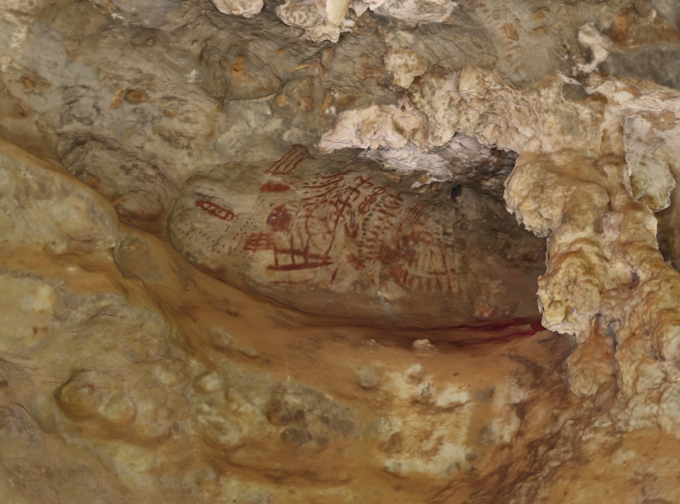
\includegraphics[height=5cm, keepaspectratio]{img/reality e fotogrametria processo/desenho bom retroprojeção.png}
        \caption{Modelo simplificado com reprojeção \\ de textura. \\
            \textbf{Fonte:} Elaborado pelo autor.}
        \label{fig:desenho bom}
    \end{minipage}
\end{figure}

  \section{Reprojeção de textura do modelo de alta resolução para o modelo simplificado, mantendo a qualidade visual.} 
  
Para manter a qualidade visual do modelo simplificado, foi aplicada a técnica de reprojeção de textura \ref{fig:desenho bom}. Essa técnica permite utilizar a textura do modelo original de alta qualidade no modelo simplificado, resultando em um equilíbrio ideal entre detalhamento visual e peso computacional. Primeiro é feito o processo de \textit{unwrap}, que pode ser traduzido como "desdobramento UV" ou "mapeamento UV" (Figura \ref{fig:unwrap}). Esta etapa minimiza distorções e sobreposições, garantindo que a textura se encaixe ao objeto 3D de forma realística, facilitando a transposição de texturas de um modelo para o outro. 
\begin{figure}[H]
        \centering
        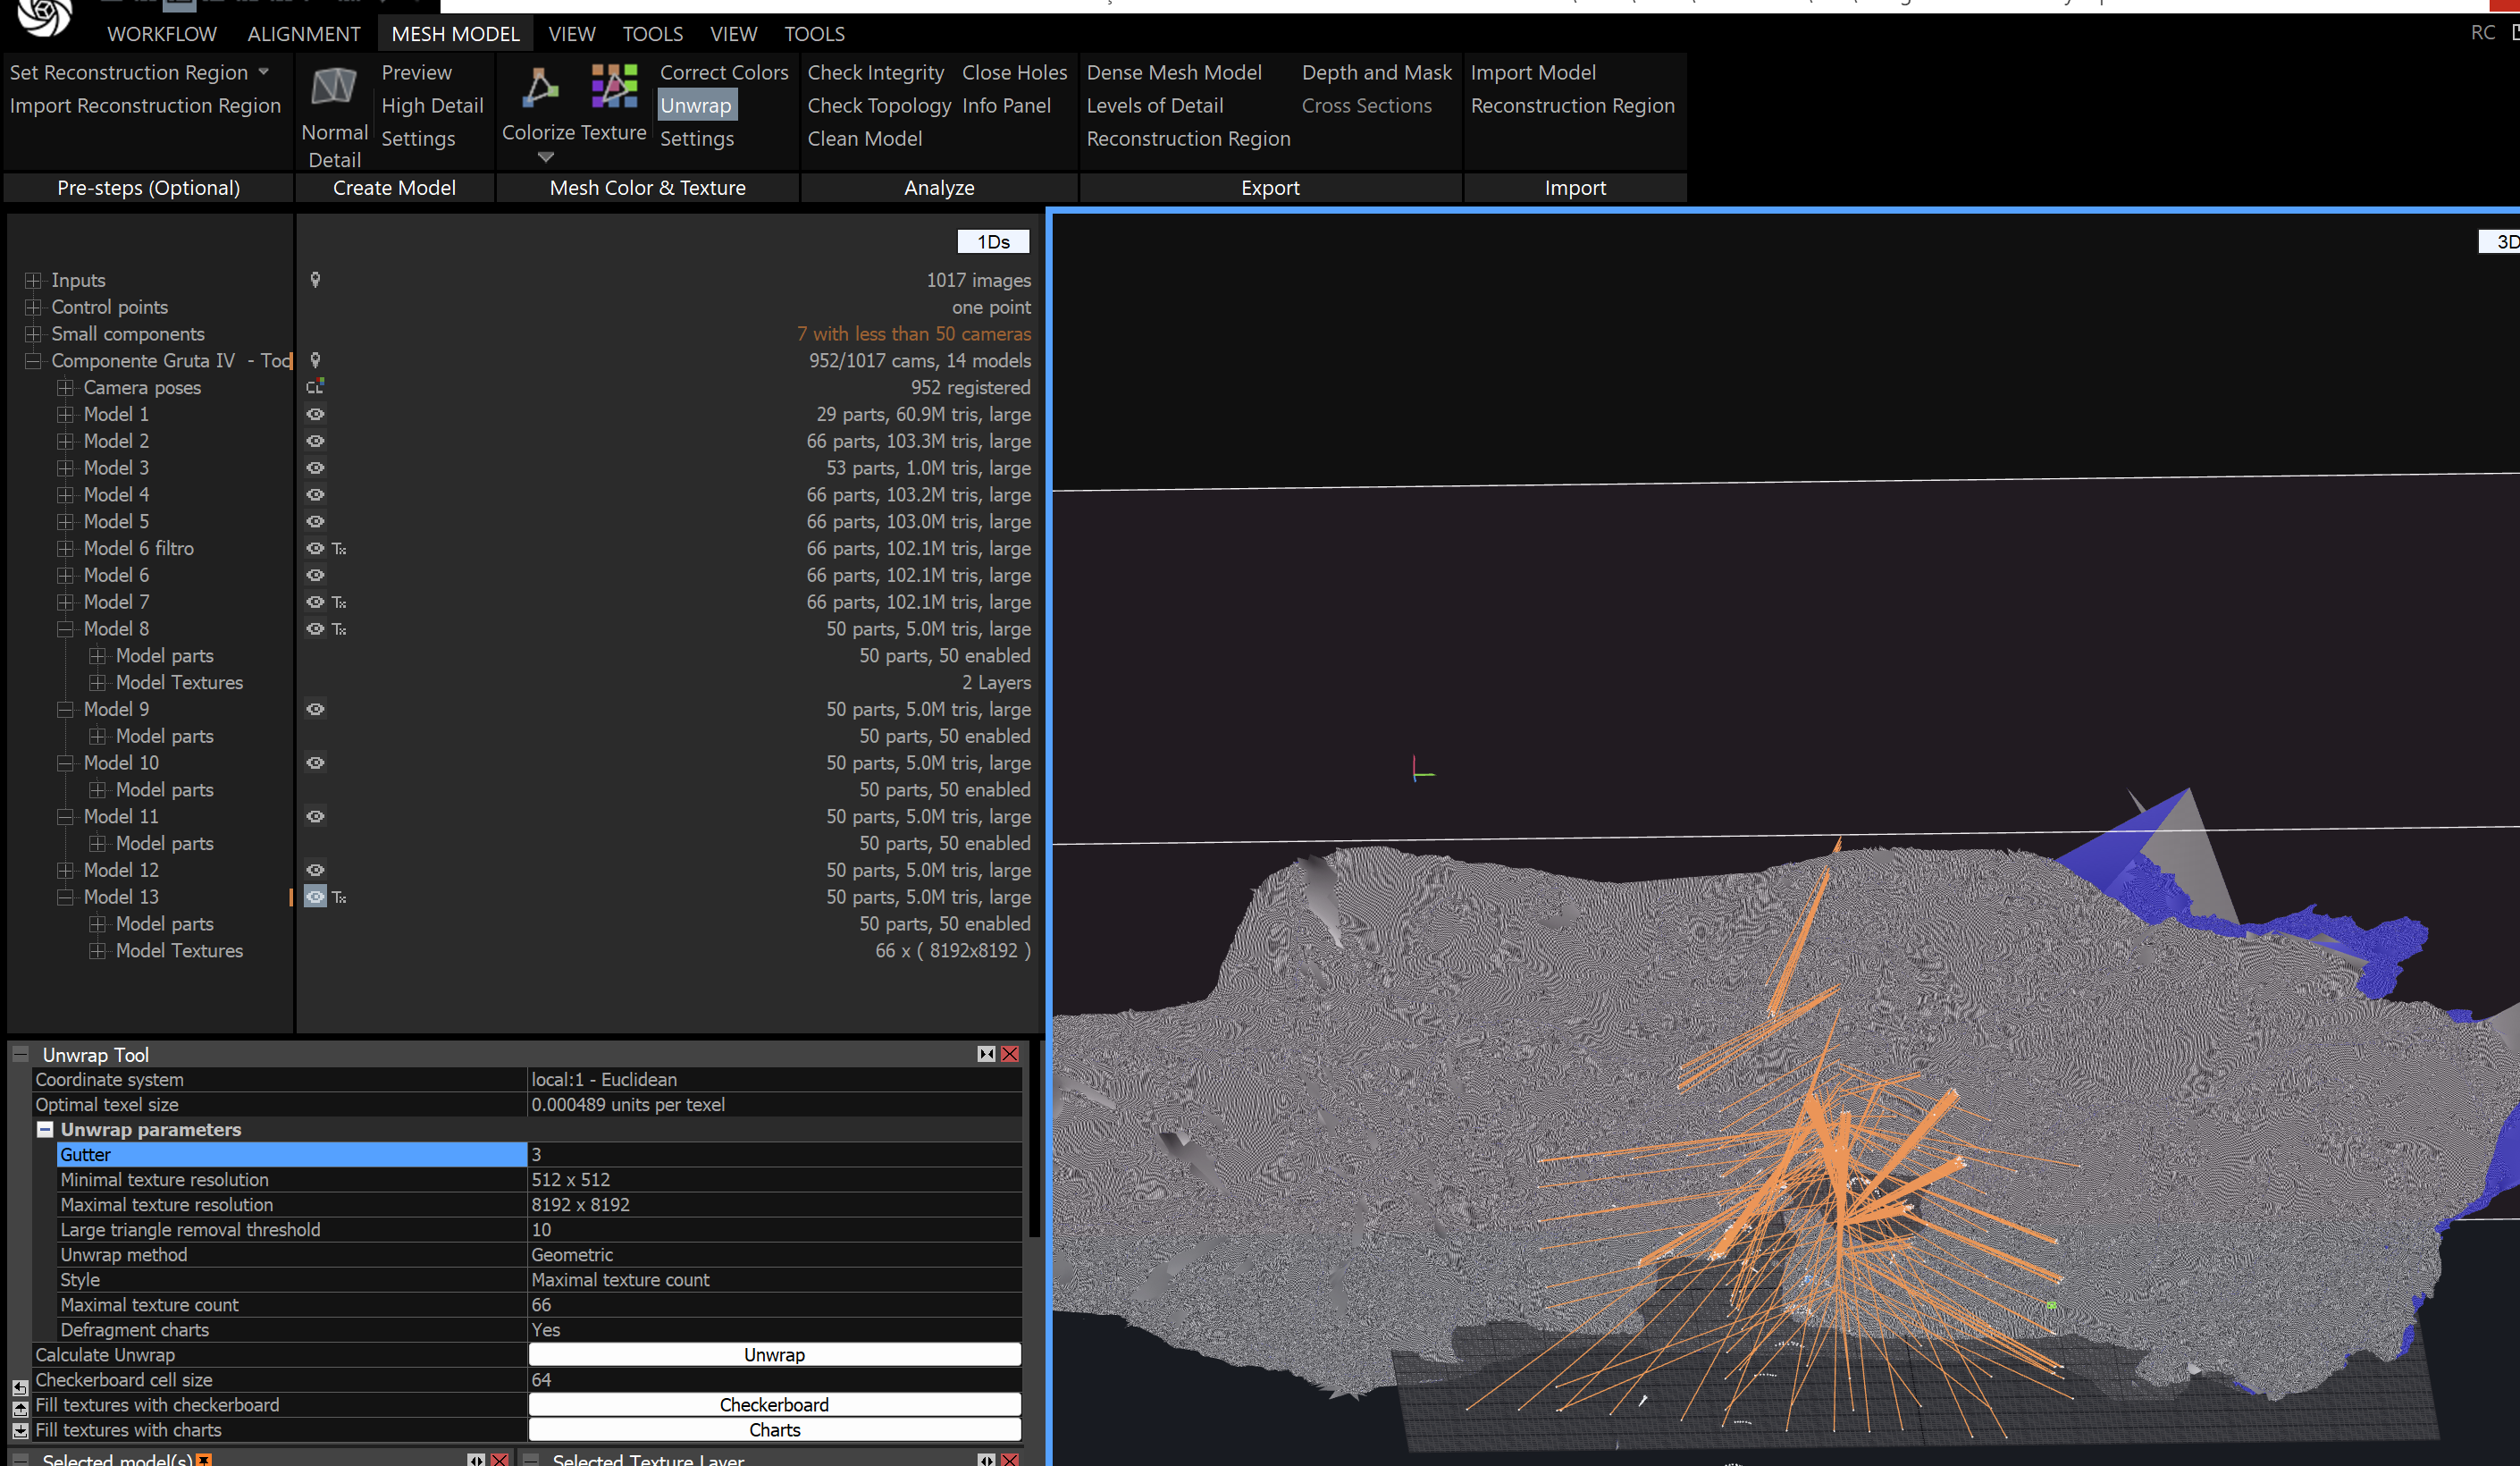
\includegraphics[height=8cm, keepaspectratio]{img/reality e fotogrametria processo/unwrap.png}
        \caption{Processo de Mapeamento UV. \\
            \textbf{Fonte:} Elaborado pelo autor.}
        \label{fig:unwrap}
\end{figure}

Todo o processo no Reality Capture é demorado e cada etapa pode consumir várias horas. Um dos processos mais rápidos foi o de reprojeção de textura que demorou cerca de apenas 2 horas utilizando um Galaxybook 4 ultra com 32 Gigas de memória RAM, placa de Vídeo NVIDIA 4070 e processador Intel(R) Core(TM) Ultra 9 185H   2.50 GHz com 22 núcleos. Na Figura \ref{fig:reprojecao tempo} pode ser vista uma captura de tela do software processando a reprojeção.
\begin{figure}[H]
        \centering
        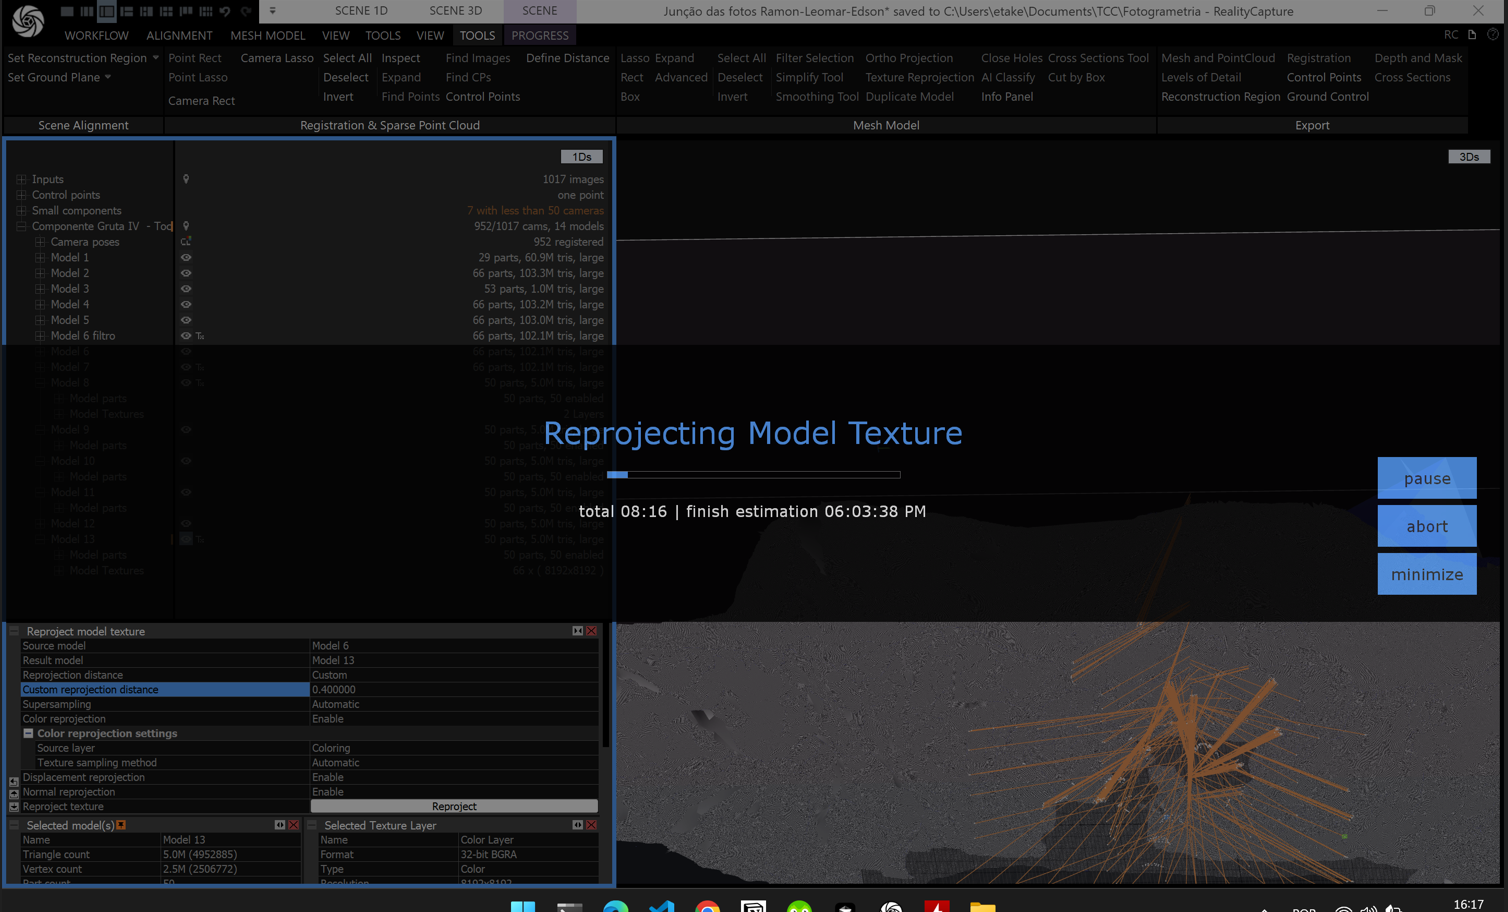
\includegraphics[height=8cm, keepaspectratio]{img/reality e fotogrametria processo/reprojeção.png}
        \caption{Processamento da reprojeção de textura. \\
            \textbf{Fonte:} Elaborado pelo autor.}
        \label{fig:reprojecao tempo}
\end{figure}


\end{enumerate}
\subsection{Considerações Finais do Ciclo 1}
O processo de fotogrametria no Reality Capture demonstrou ser uma ferramenta poderosa para a geração de modelos 3D detalhados. A combinação de técnicas como a simplificação de malhas e a reprojeção de textura permitiu criar modelos otimizados para uso em softwares como a Unreal Engine, mantendo alta qualidade visual. Este fluxo de trabalho é essencial para aplicações em um ambiente virtual, a qual é a próxima etapa.

\section{Ciclo 2: Construção do Ambiente Virtual na Unreal Engine}
\label{sec:ciclo2_unreal}
A escolha da plataforma Unreal Engine 5.4 para a criação do ambiente virtual 3D se justifica pela sua capacidade de gerar experiências imersivas e interativas. O Unreal Engine é um motor de criação de jogos amplamente utilizado na indústria de jogos, cinema e arquitetura. A plataforma oferece recursos como simulação de luz, movimentações de câmera e personagens, e a possibilidade de interagir com os elementos do ambiente, tornando o ambiente virtual 3D mais realista e envolvente \citep{silva2022realidade}.

\textbf{Objetivo}: Criar um ambiente virtual interativo e imersivo.

\textbf{Processo}:
\begin{itemize}
    \item Importação do modelo 3D para a Unreal Engine.
    \item Aplicação de texturas, iluminação e configurações de física.
    \item Implementação da navegação do usuário e interações.
\end{itemize}

\section{Ciclo 3: Prototipação do Novo Site}
\label{sec:ciclo3_prototipacao}

\textbf{Objetivo}: Criar um protótipo de alta fidelidade para o site.

\textbf{Processo}:
\begin{itemize}
    \item Criação de uma identidade visual
    \item Definição da arquitetura da informação e wireframes.
    \item Desenvolvimento do protótipo no Figma.
    \item Validação do design com stakeholders.
\end{itemize}

\begin{figure}[H]
    \centering
    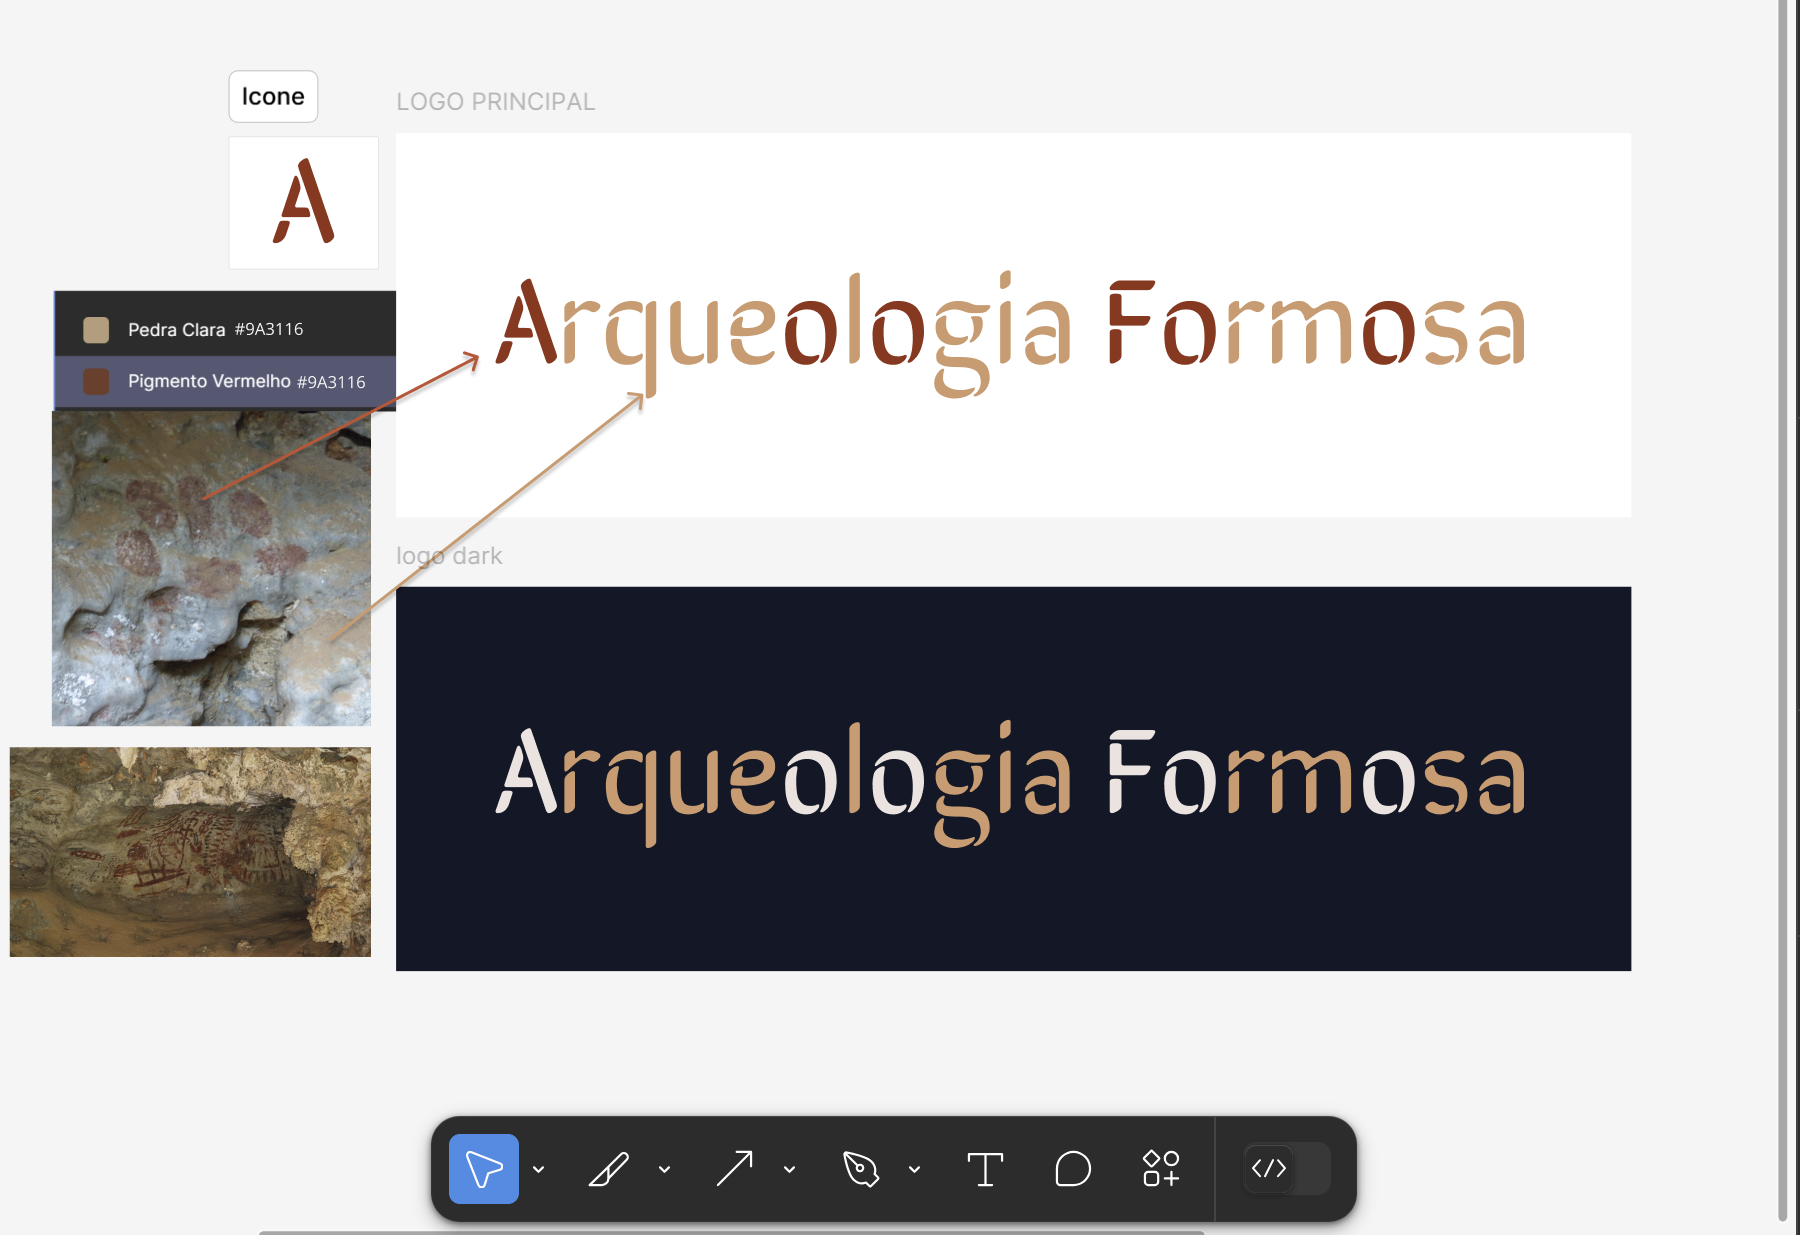
\includegraphics[height=8cm, keepaspectratio]{img/Protótipo/logo.png}
    \caption{ Logo do site Arqueologia Formosa inspirada nos pictoglifos e rochas da Lapa da Pedra. \\
        \textbf{Fonte:} Elaborado pelo autor.}
    \label{fig:logo_arqueologia_formosa}
\end{figure}

\begin{figure}[H]
    \centering
    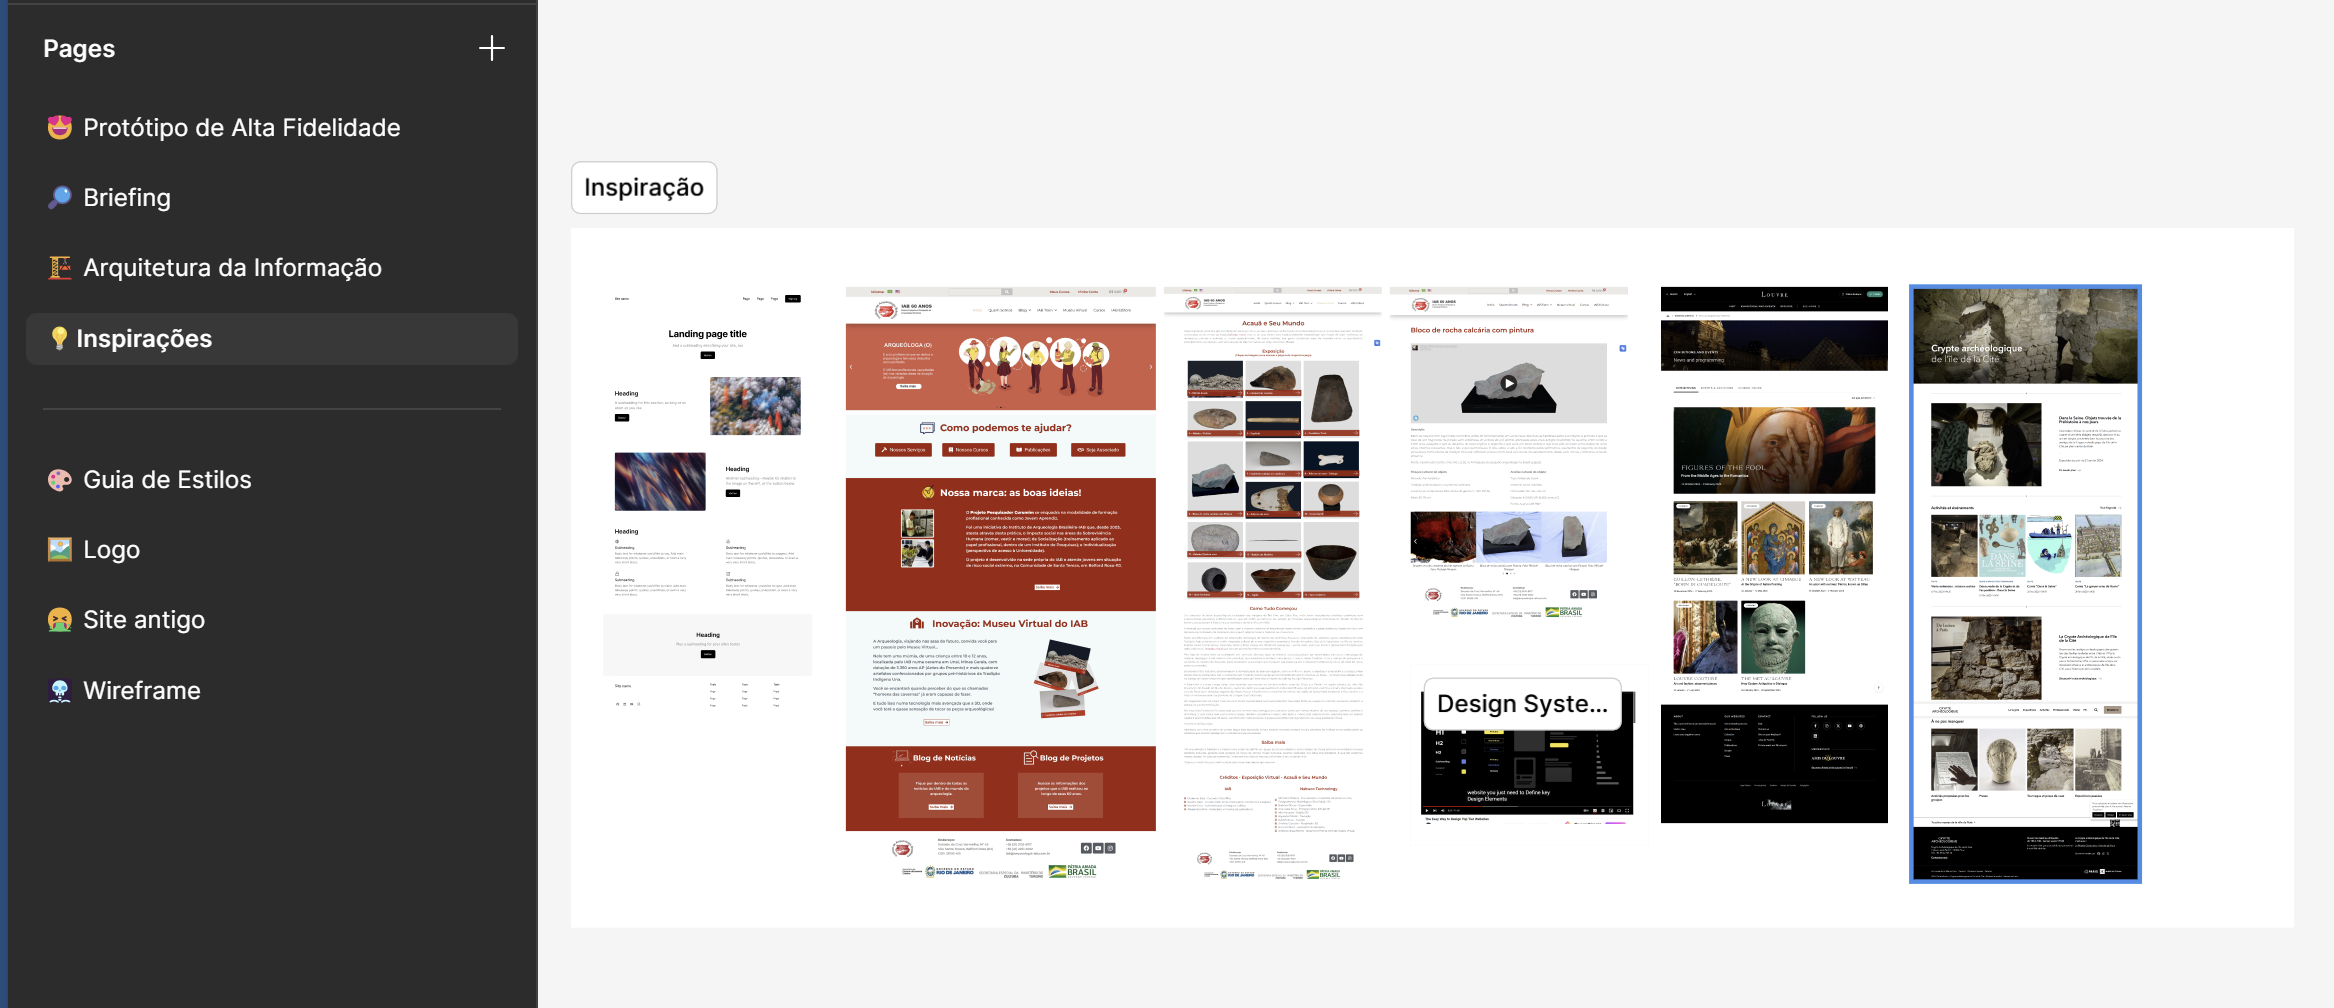
\includegraphics[height=6cm, keepaspectratio]{img/Protótipo/inspiração.png}
    \caption{ Inspirações de outros sites de arqueologia, sites com boa estética, \\ paleta de cores ou forma atrativa. \\
        \textbf{Fonte:} Elaborado pelo autor.}
    \label{fig:inpirações}
\end{figure}

\begin{figure}[H]
    \centering
    \begin{minipage}[b]{0.48\textwidth}
        \centering
        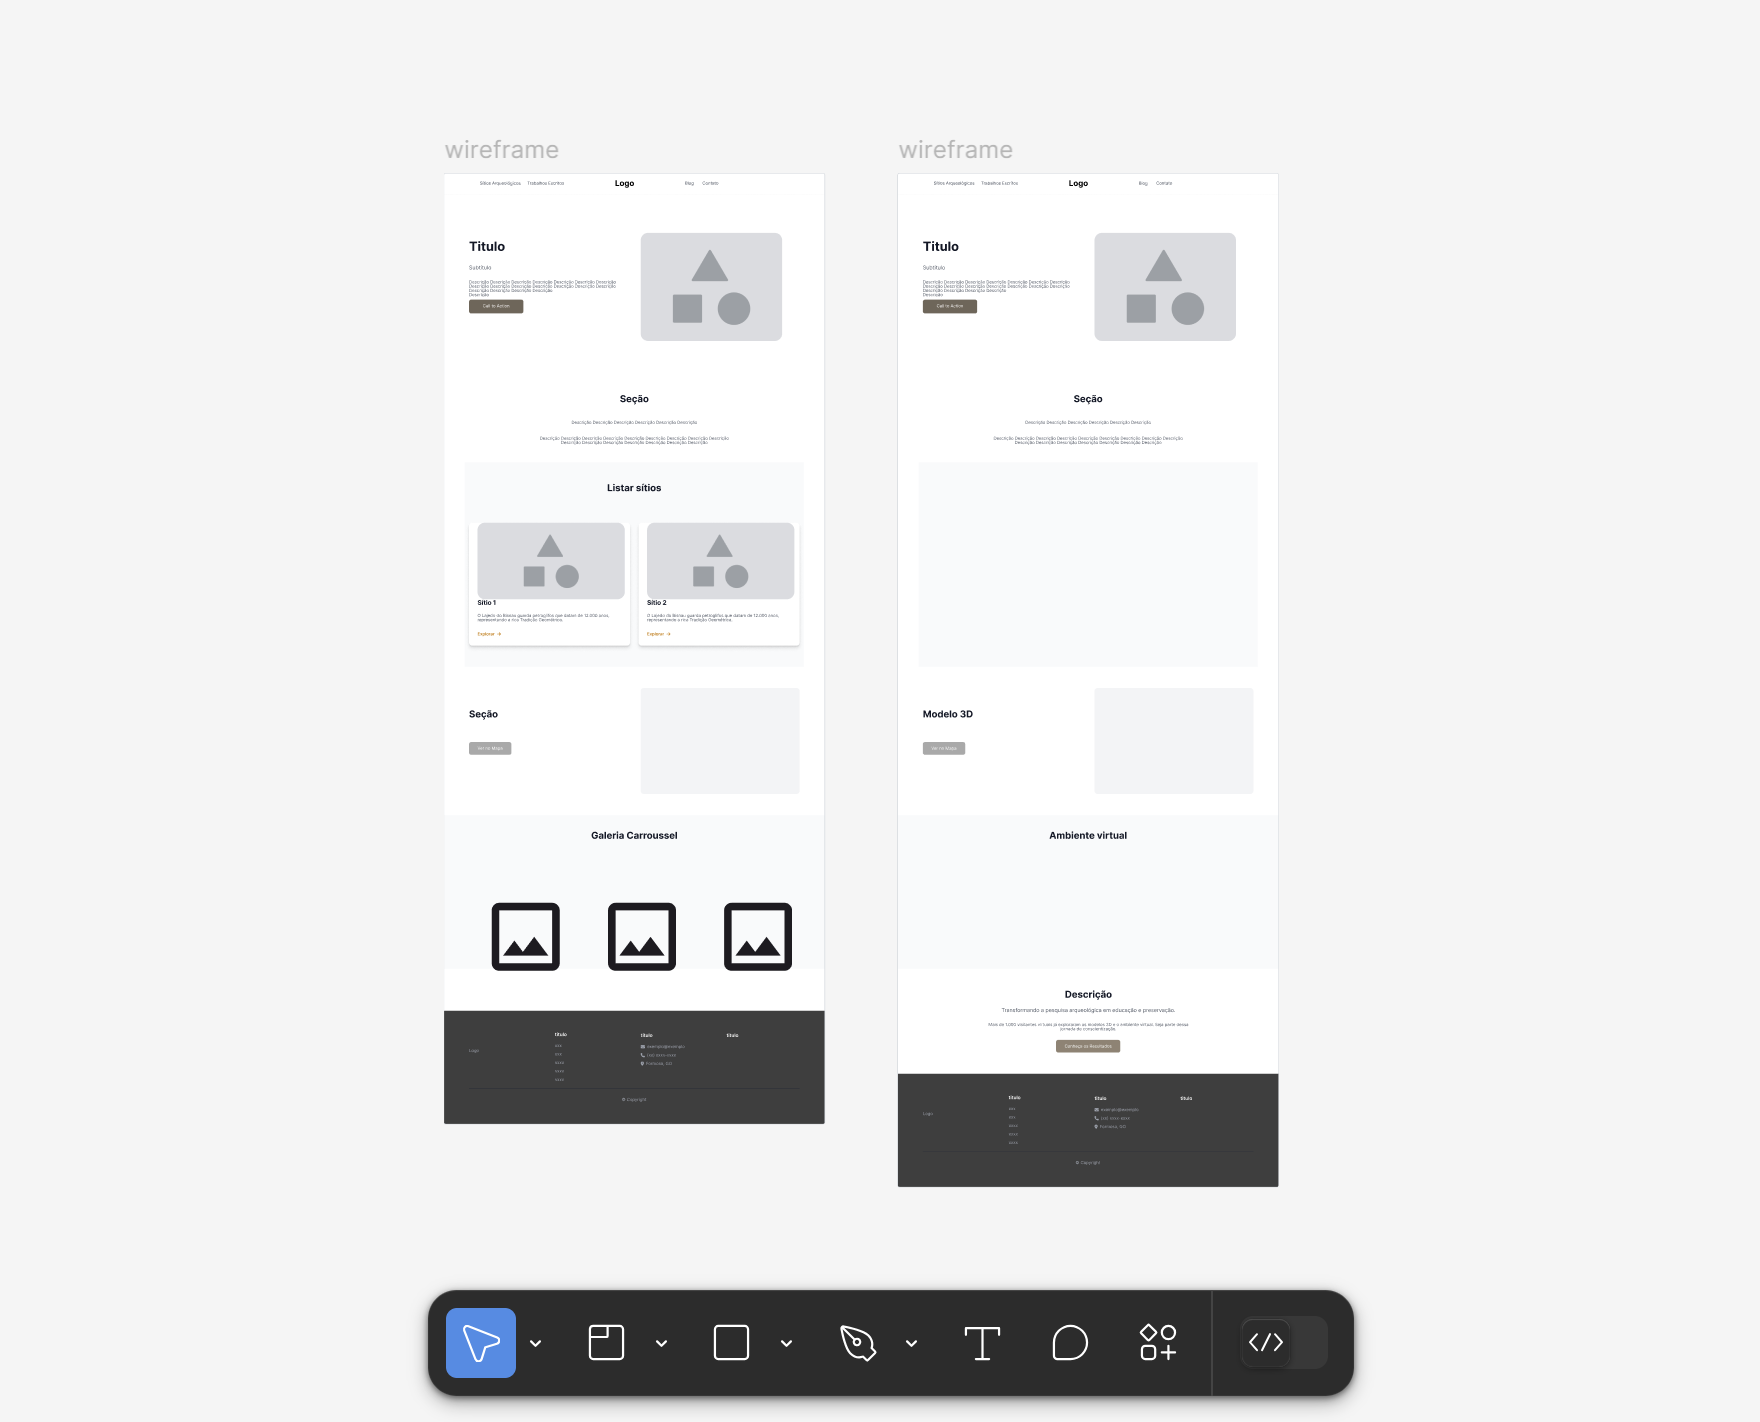
\includegraphics[height=8cm, keepaspectratio]{img/Protótipo/wireframes.png}
        \caption{Wireframes de baixa fidelidade no Figma. \\
            \textbf{Fonte:} Elaborado pelo autor.}
        \label{fig:wireframes}
    \end{minipage}
    \hfill
    \begin{minipage}[b]{0.48\textwidth}
        \centering
        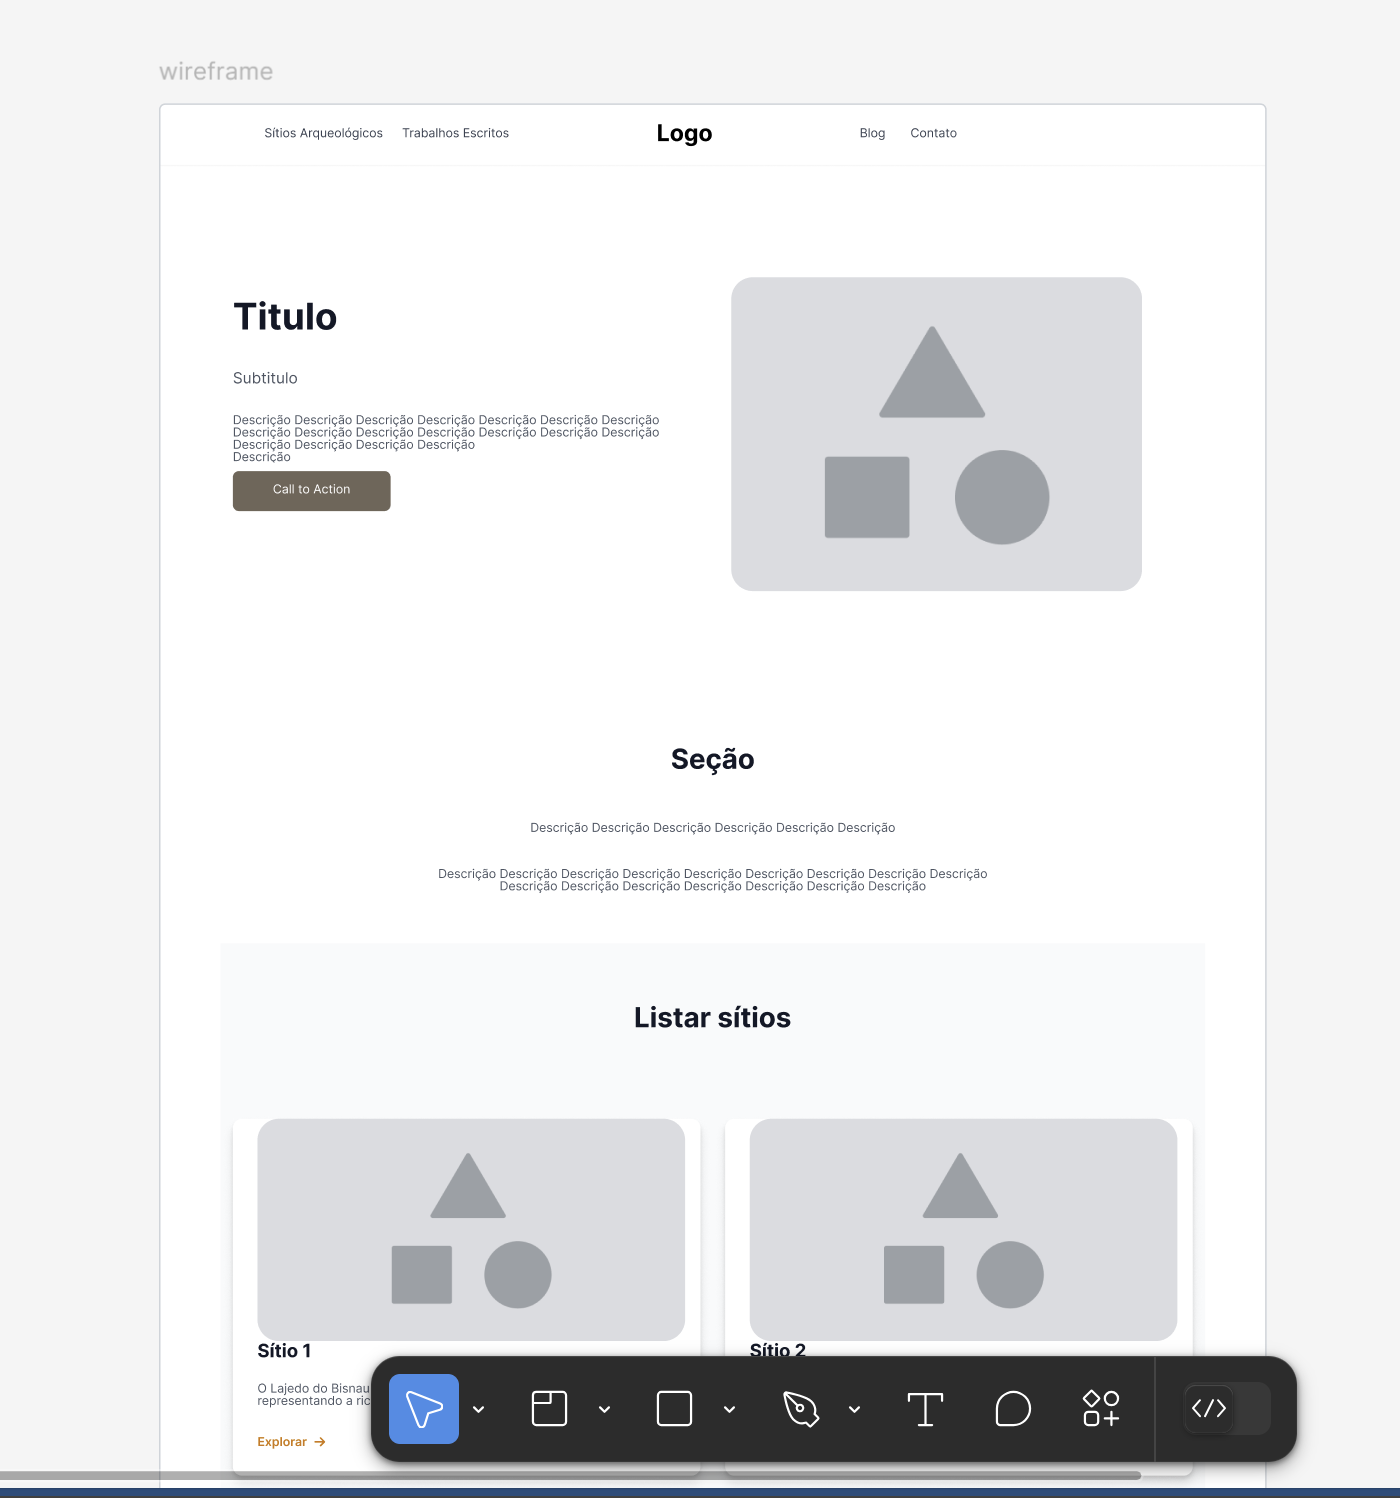
\includegraphics[height=8cm, keepaspectratio]{img/Protótipo/wireframe.png}
        \caption{Wireframe de baixa fidelidade no Figma. \\
            \textbf{Fonte:} Elaborado pelo autor.}
        \label{fig:wireframe}
    \end{minipage}
\end{figure}

\begin{figure}[H]
    \centering
    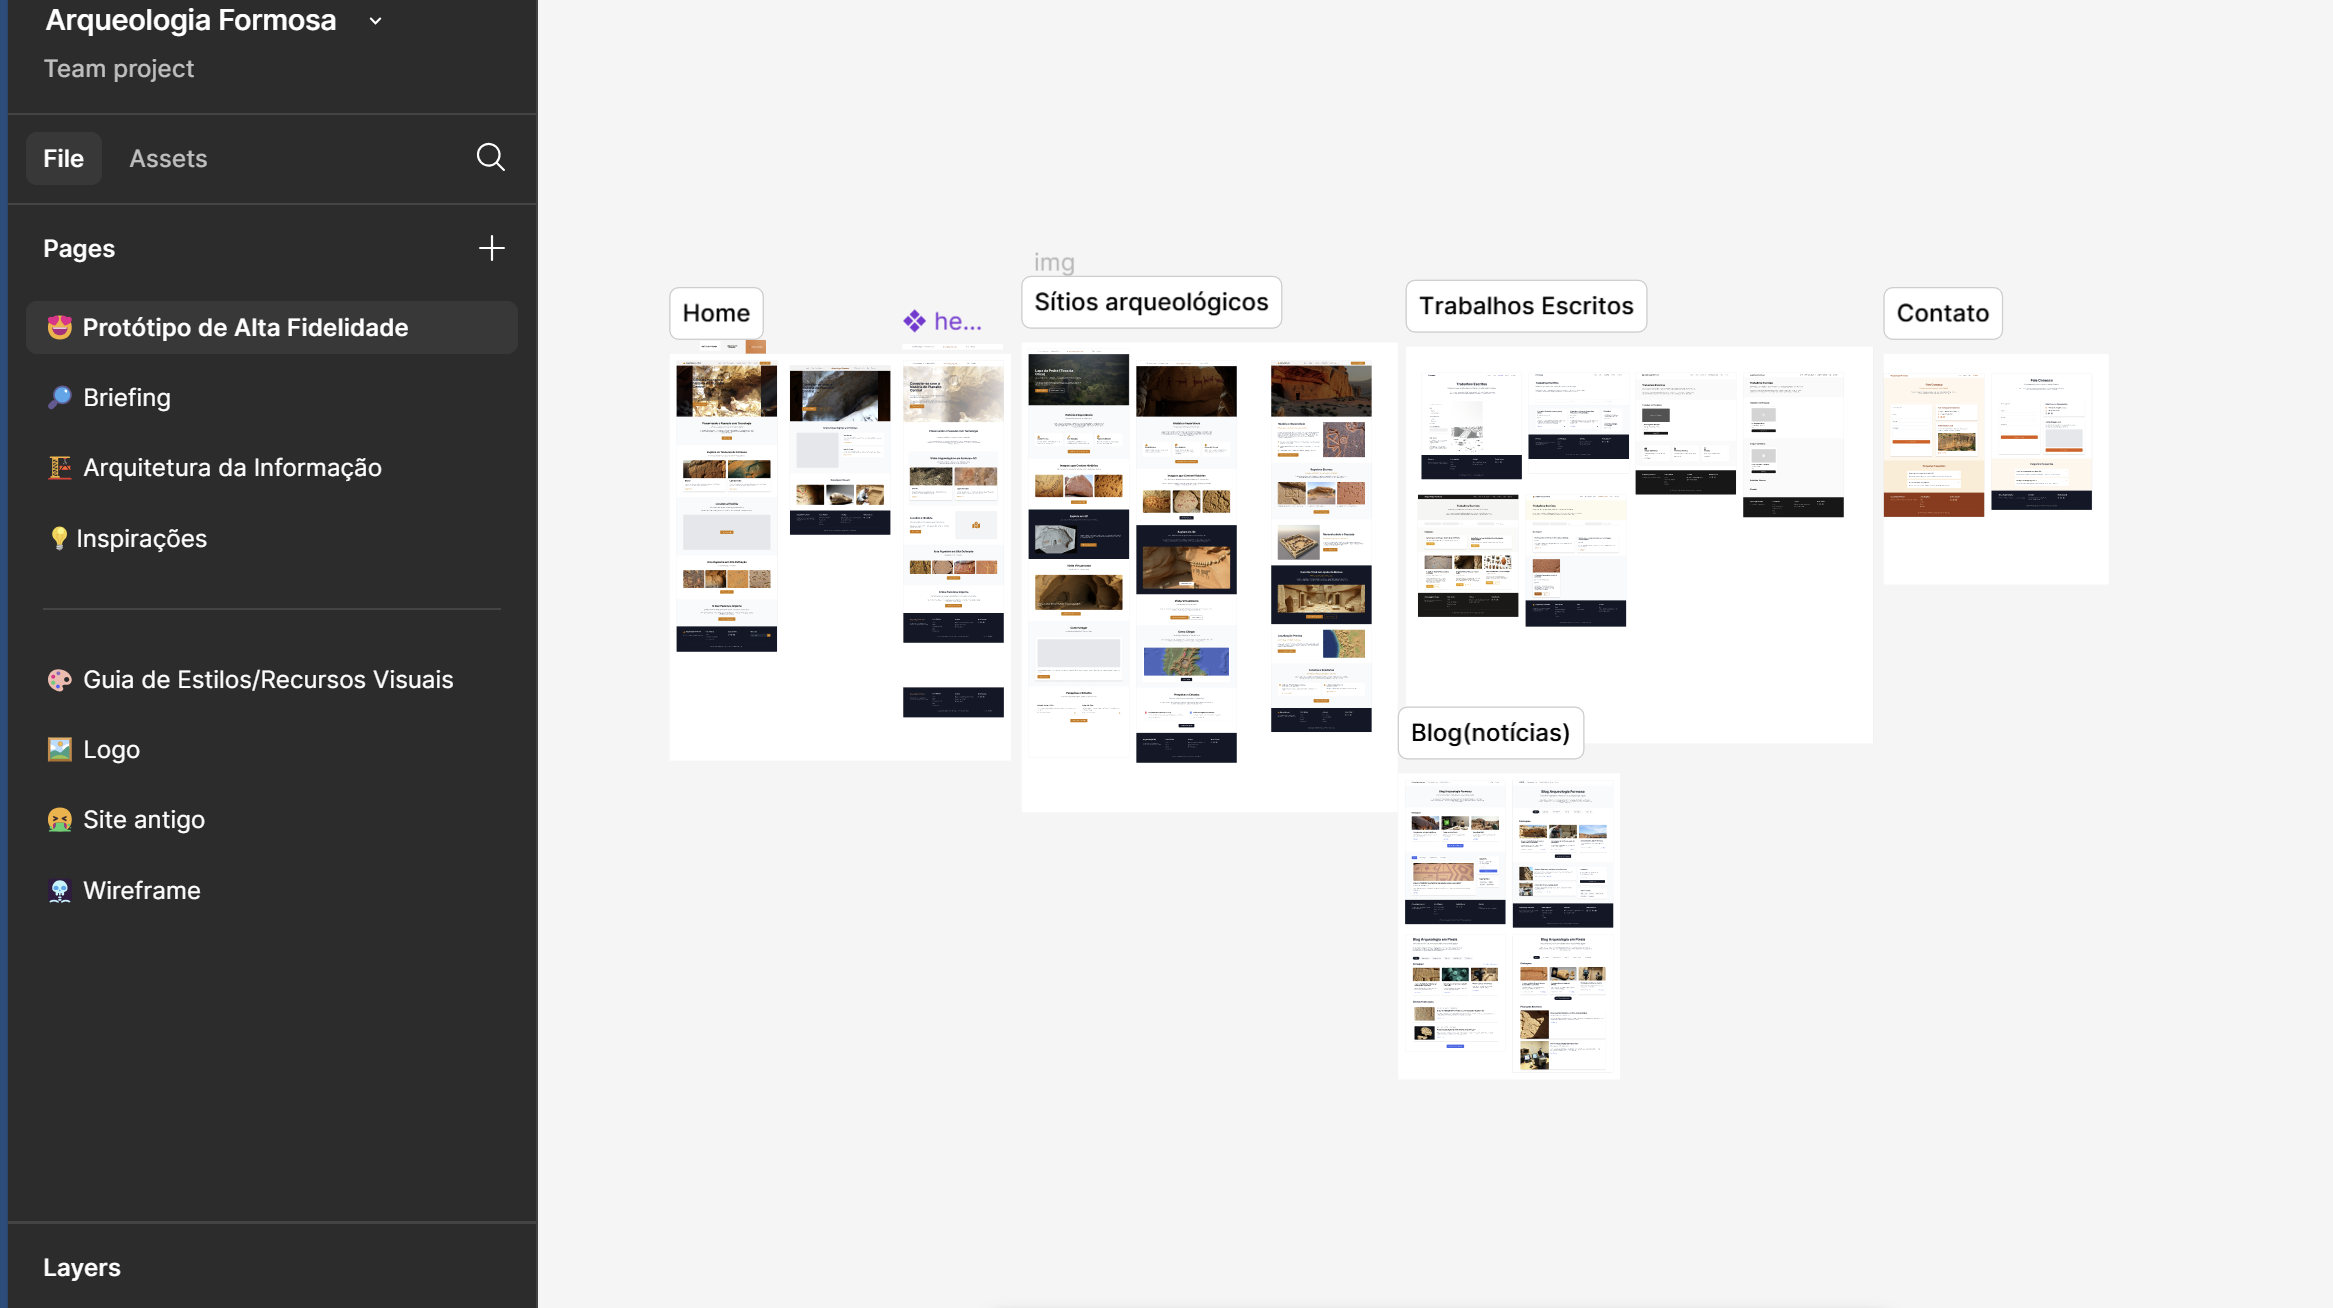
\includegraphics[height=8cm, keepaspectratio]{img/Protótipo/alta fidelidade.png}
    \caption{ Protótipos de Alta Fidelidade das telas principais no Figma. \\
        \textbf{Fonte:} Elaborado pelo autor.}
    \label{fig:prototipo_alta_fidelidade}
\end{figure}

\begin{figure}[H]
    \centering
    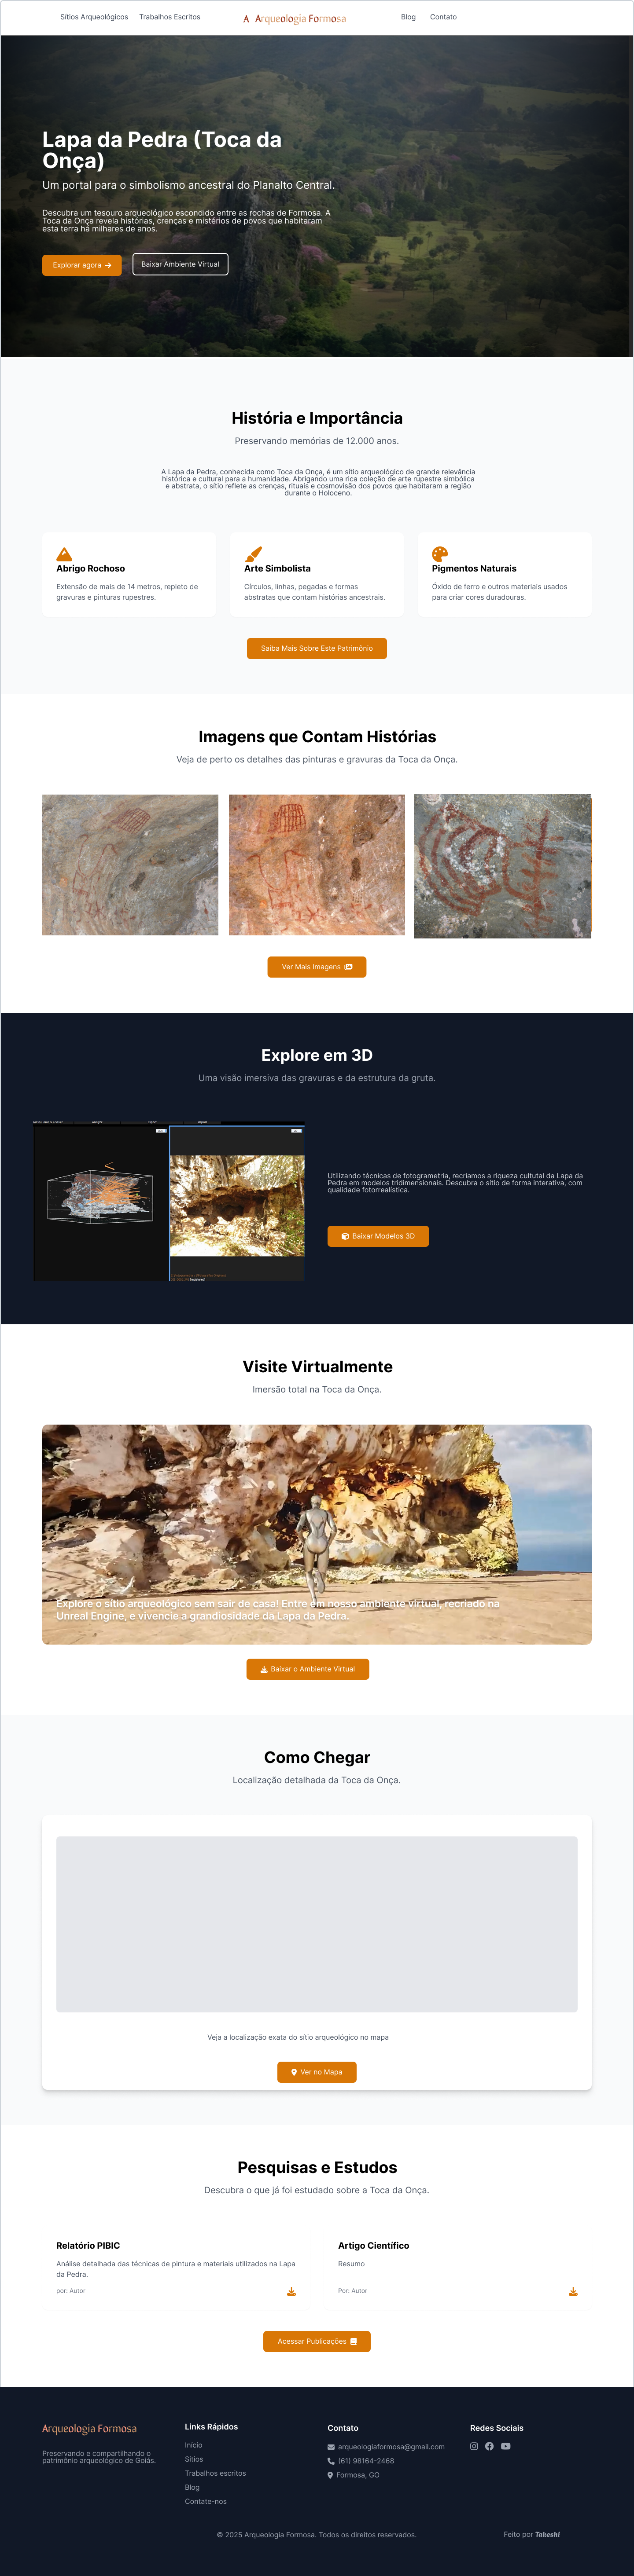
\includegraphics[height=20cm, keepaspectratio]{img/Protótipo/prototipo alta fidelidade toca da onça.png}
    \caption{ Protótipos de Alta Fidelidade das telas principais no Figma. \\
        \textbf{Fonte:} Elaborado pelo autor.}
    \label{fig:prototipo_alta_fidelidade}
\end{figure}


\begin{figure}[H]
    \centering
    \begin{minipage}[b]{0.48\textwidth}
        \centering
        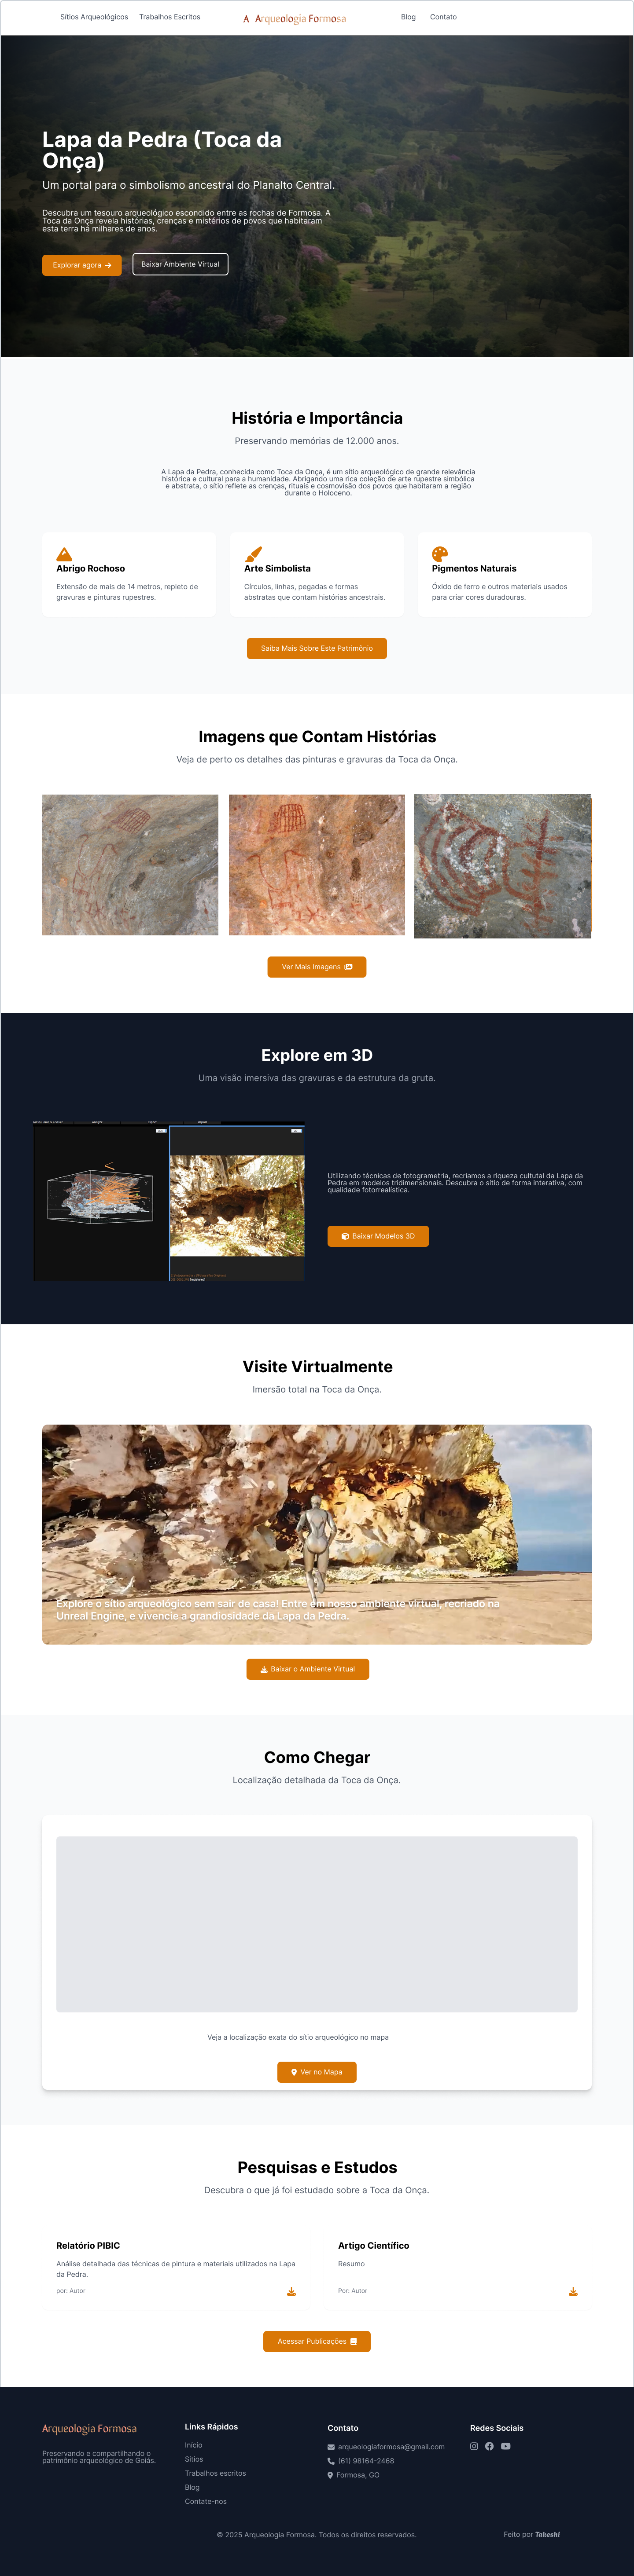
\includegraphics[height=22cm, keepaspectratio]{img/Protótipo/prototipo alta fidelidade toca da onça.png}
        \caption{Wireframes de baixa fidelidade no Figma. \\
            \textbf{Fonte:} Elaborado pelo autor.}
        \label{fig:wireframes}
    \end{minipage}
    \hfill
    \begin{minipage}[b]{0.48\textwidth}
        \centering
        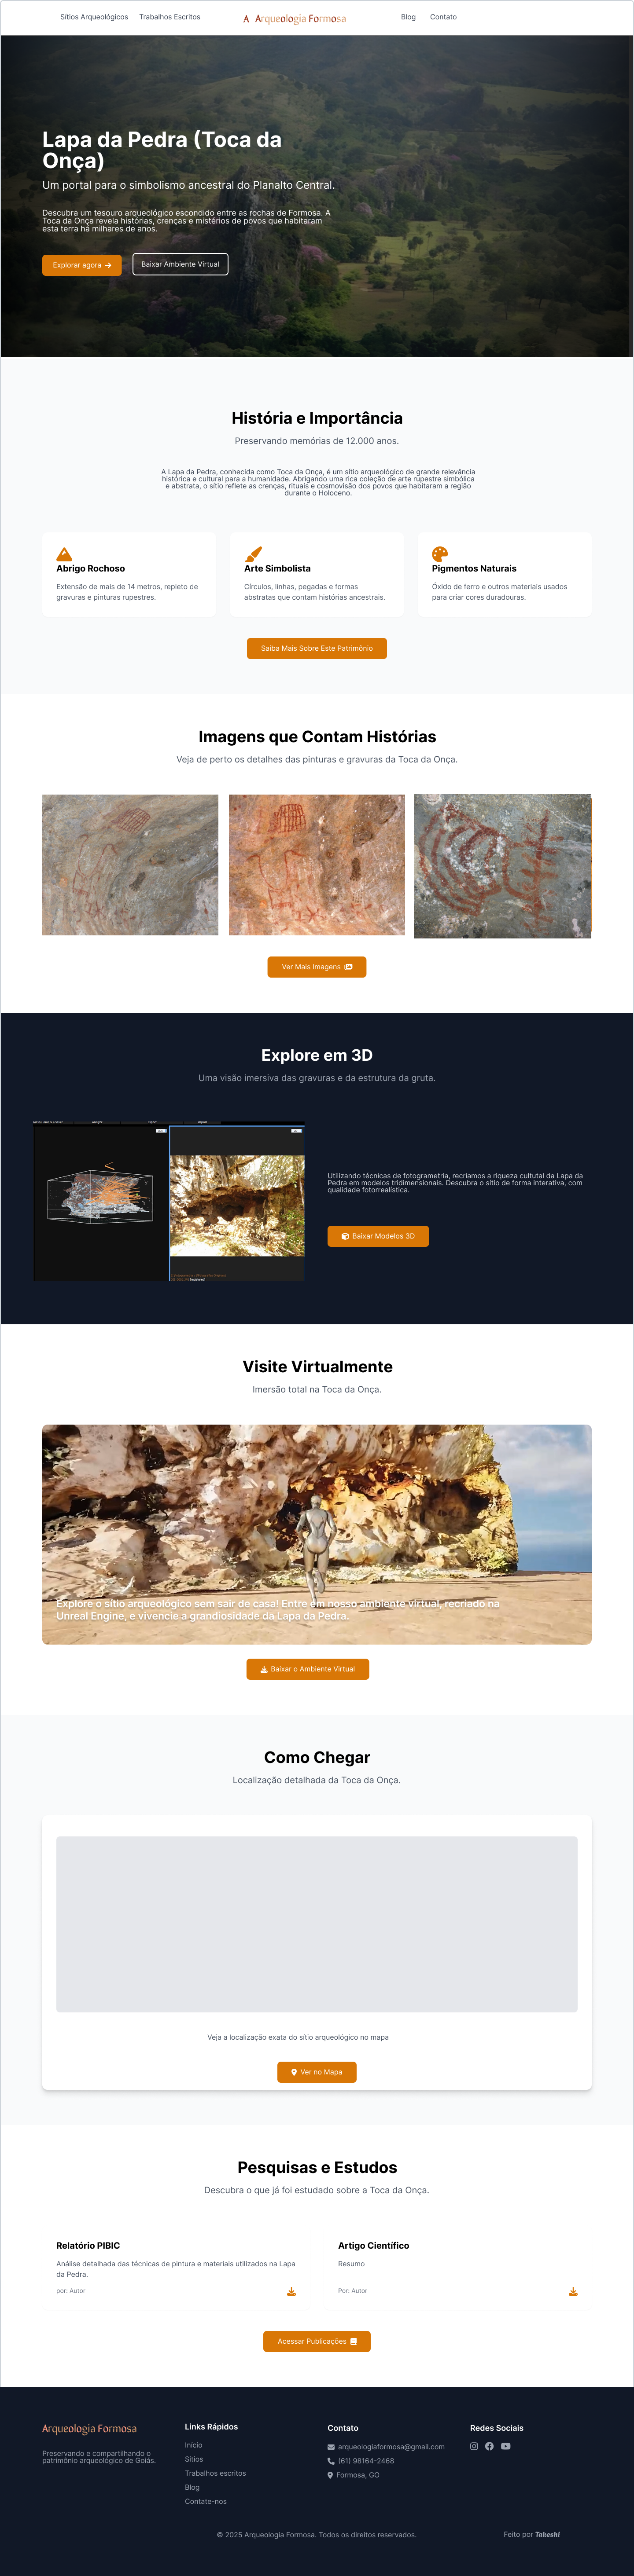
\includegraphics[height=24cm, keepaspectratio]{img/Protótipo/prototipo alta fidelidade toca da onça.png}
        \caption{Wireframe de baixa fidelidade no Figma. \\
            \textbf{Fonte:} Elaborado pelo autor.}
        \label{fig:wireframe}
    \end{minipage}
\end{figure}

\section{Ciclo 4: Desenvolvimento do Novo Site}
\label{sec:ciclo4_desenvolvimento}

\textbf{Objetivo}: Implementar o site final baseado no protótipo validado.

\textbf{Processo}:
\begin{itemize}
    \item Configuração do ambiente \textit{JAMstack} com Next.js, Sanity e Schema UI.
    \item Implementação de páginas e funcionalidades.
    \item Otimizações de performance e SEO.
    \item Testes e ajustes finais.
\end{itemize}

\textbf{Imagens e Evidências}:
Adicionar prints das telas implementadas, código relevante e testes realizados.

\section{Avaliação e Testes}
\label{sec:avaliacao_testes}

\textbf{Objetivo}: Garantir que a solução atenda aos requisitos definidos.

\textbf{Processo}:
\begin{itemize}
    \item Testes de usabilidade.
    \item Validação heurística.
    \item Avaliação de performance e responsividade.
\end{itemize}

\textbf{Imagens e Evidências}:
Adicionar capturas de relatórios de testes, feedbacks coletados e ajustes realizados.

\section{Publicação e Deploy}
\label{sec:publicacao_deploy}

\textbf{Objetivo}: Tornar o projeto acessível ao público.

\textbf{Processo}:
\begin{itemize}
    \item Deploy na Vercel e disponibilização pública do site (Figura \ref{fig:deploy_vercel}). 
\begin{figure}[H]
    \centering
    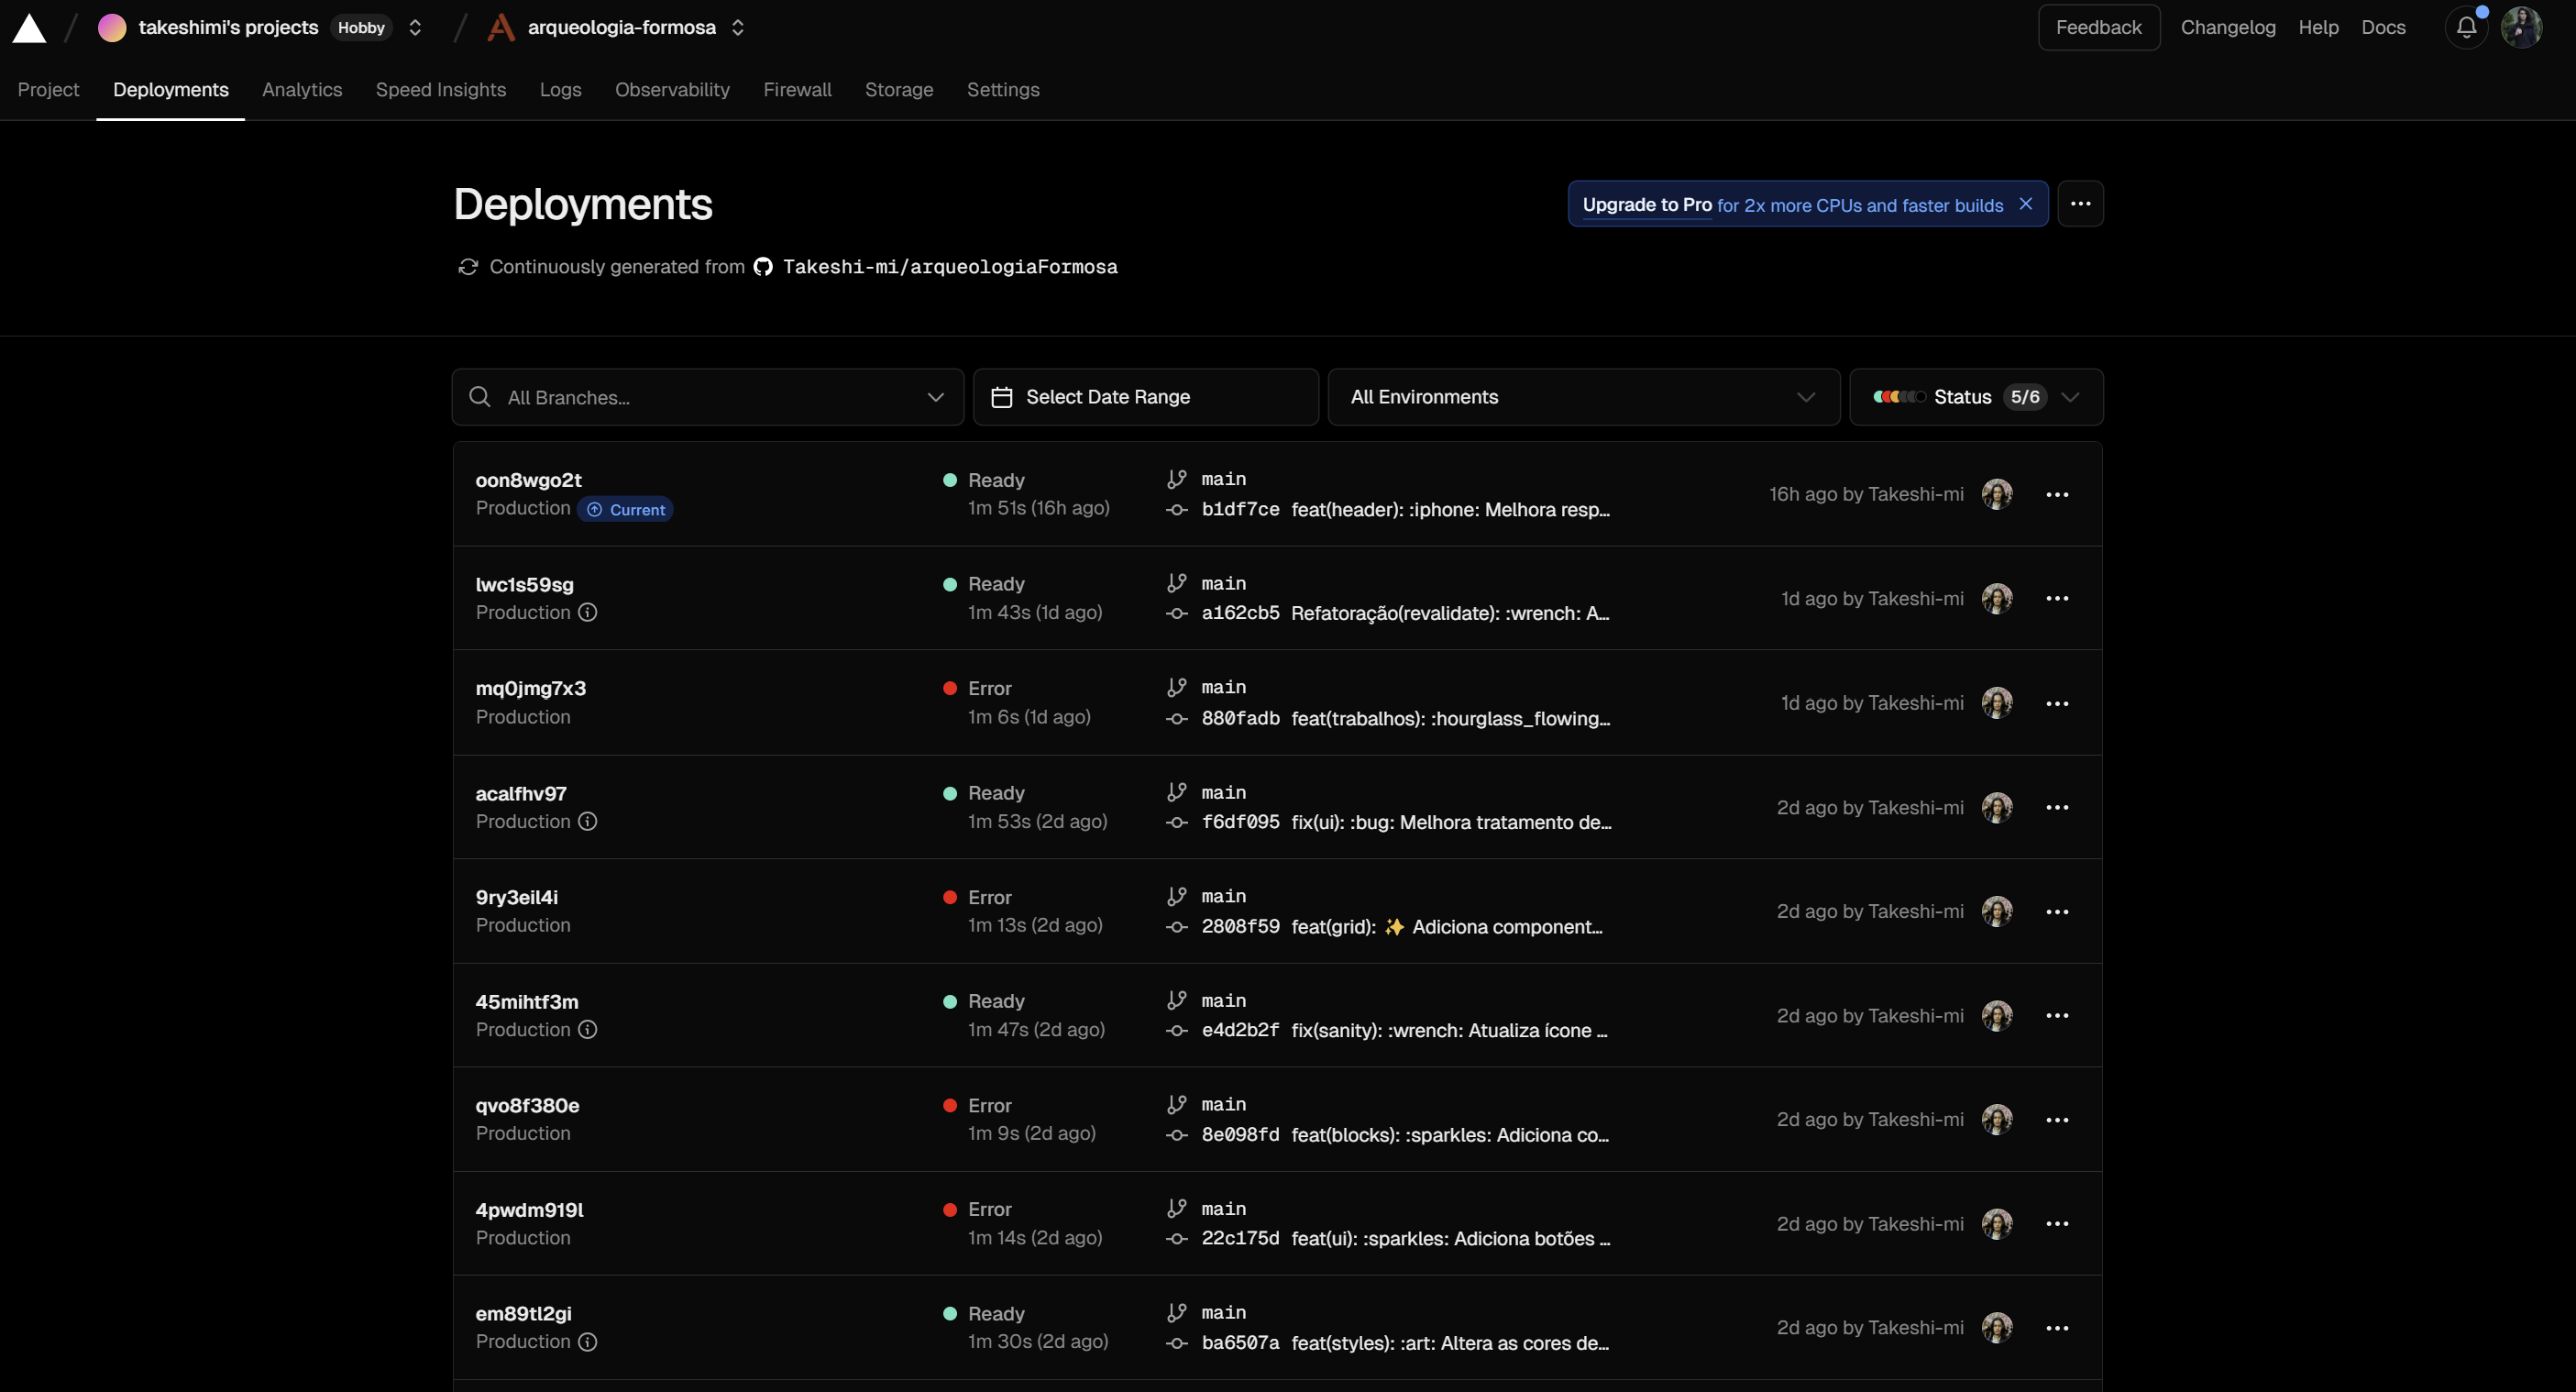
\includegraphics[height=8cm, keepaspectratio]{img/Deploy/deploy_vercel.png}
    \caption{ Captura de tela do processo de deploy na vercel com esteira CI/CD integrada. \\
        \textbf{Fonte:} Elaborado pelo autor.}
    \label{fig:deploy_vercel}
\end{figure}

    \item Registro de domínio pelo \href{www.registro.br}{Registro.br}, que é o departamento do NIC.br responsável pelas atividades de registro e manutenção dos nomes de domínios que usam o .br. Essa escolha garante maior confiabilidade, identidade nacional e melhor indexação nos mecanismos de busca (Figura \ref{fig:dominio_registro_br}).
\begin{figure}[H]
    \centering
    \includegraphics[height=8cm, keepaspectratio]{img/Deploy/domínio-registro.br.png}
    \caption{ Domínio disponível para compra no site \href{www.registro.br}{Registro.br}. \\
        \textbf{Fonte:} Elaborado pelo autor.}
    \label{fig:dominio_registro_br}
\end{figure}

    \item Configuração de DNS para apontar o domínio para a Vercel (Figura \ref{fig:dns}).
\begin{figure}[H]
    \centering
    \includegraphics[height=8cm, keepaspectratio]{images/dns_config.png}
    \caption{ Configuração de DNS para apontar o domínio para a Vercel. \\
        \textbf{Fonte:} Elaborado pelo autor.}
    \label{fig:dns}
\end{figure}

\end{itemize}




 \chapter{Resultados}
\label{cap:resultados}

\section{Introdução}
Este capítulo apresenta os resultados obtidos com o desenvolvimento do site e do ambiente virtual, correlacionando-os diretamente aos objetivos estabelecidos no início deste trabalho. Demonstra-se como cada objetivo foi atendido, com destaque para as melhorias implementadas em relação ao estado anterior do site e a criação de um ambiente virtual \gls{3d} interativo para a divulgação e preservação da arte rupestre.

\section{Objetivo Geral}
O objetivo geral deste trabalho foi desenvolver uma plataforma web e um ambiente virtual \gls{3d} que promovam a preservação, divulgação e acesso educativo à arte rupestre da Lapa da Pedra. Esse objetivo foi atingido por meio da entrega de:
\begin{itemize}
    \item Um novo site moderno, acessível e responsivo, que organiza as informações de forma clara e permite fácil navegação.
    \item Um ambiente virtual interativo que possibilita a visualização detalhada das pinturas rupestres e oferece uma experiência imersiva aos usuários.
    \item Funcionalidades que tornam o site útil para educadores, pesquisadores e o público geral, como galeria de imagens, acesso a modelos \gls{3d} e artigos publicados.
\end{itemize}

As seções a seguir detalham como os objetivos específicos foram atendidos.

\section{Objetivos Específicos}

\subsection{Análise Heurística de Usabilidade: Problemas Identificados no Site Antigo}
Um dos objetivos específicos era realizar uma análise heurística de usabilidade do antigo site "Arqueologia Formosa". Essa análise foi conduzida com base nas heurísticas de Nielsen, avaliando aspectos como navegabilidade, eficiência e consistência. Os principais problemas identificados foram:
\begin{itemize}
    \item Layout desorganizado, dificultando a localização de informações importantes.
    \item Falta de responsividade para dispositivos móveis.
    \item Ausência de funcionalidades modernas, como busca eficiente e compartilhamento em redes sociais.
\end{itemize}

Esses problemas foram utilizados como base para o planejamento do novo site, garantindo que as falhas do sistema anterior fossem corrigidas. A análise heurística também guiou a priorização das melhorias implementadas.

\subsection{Desenvolvimento de um Novo Site com Design Centrado no Usuário (\gls{ux})}
O novo site foi desenvolvido com tecnologias modernas (\textit{Next.js}, \textit{Tailwind CSS} e \textit{Sanity CMS}), priorizando uma experiência do usuário intuitiva e acessível. Os resultados alcançados incluem:
\begin{itemize}
    \item Design responsivo, otimizado para dispositivos móveis, desktops e tablets.
    \item Galeria de imagens organizada, com suporte para visualização ampliada.
    \item Modo escuro/claro, permitindo maior conforto visual.
    \item Implementação de padrões de acessibilidade conforme WCAG 2.1 (nível AA).
\end{itemize}

A Figura \ref{fig:site_homepage} apresenta a página inicial do novo site, evidenciando o layout moderno e a organização do conteúdo.

\begin{figure}[H]
    \centering
    % Substitua pelo caminho do arquivo de imagem
    \includegraphics[width=0.8\linewidth]{images/site_homepage.png}
    \caption{Página inicial do novo site "Arqueologia Formosa".}
    \label{fig:site_homepage}
\end{figure}

\subsection{Implementação de um Ambiente Virtual \gls{3d}}
Outro objetivo específico era implementar um ambiente virtual \gls{3d} que permitisse a visualização interativa da arte rupestre. Esse objetivo foi alcançado com o desenvolvimento de um ambiente imersivo na Unreal Engine, utilizando modelos \gls{3d} gerados por fotogrametria. Os resultados incluem:
\begin{itemize}
    \item Fidelidade visual dos modelos \gls{3d}, com texturas realistas das pinturas rupestres.
    \item Navegação interativa no ambiente, permitindo aos usuários explorar o sítio arqueológico.
    \item Empacotamento do ambiente virtual em um arquivo executável, disponibilizado para \textit{download} no site.
\end{itemize}

A Figura \ref{fig:virtual_environment} apresenta uma visão do ambiente virtual desenvolvido.

\begin{figure}[H]
    \centering
    % Substitua pelo caminho do arquivo de imagem
    \includegraphics[width=0.8\linewidth]{images/virtual_environment.png}
    \caption{Ambiente virtual desenvolvido na Unreal Engine.}
    \label{fig:virtual_environment}
\end{figure}


\section{Testes e Validação}

\subsection{Usabilidade}
Os testes de usabilidade foram realizados com base nas heurísticas de Nielsen e Kaniasty. Os seguintes pontos foram avaliados:
\begin{itemize}
    \item Facilidade de navegação no site e no ambiente virtual.
    \item Eficiência na interação com a galeria de imagens e o ambiente virtual.
    \item Satisfação dos usuários com o design e as funcionalidades implementadas.
\end{itemize}


\begin{table}[H]
\centering
\caption{Resultados dos testes de usabilidade.}
\label{tab:usabilidade}
\begin{tabularx}{\textwidth}{|l|X|X|} % Ajusta a largura da tabela ao texto
\hline
\textbf{Critério Avaliado} & \textbf{Pontuação Média} & \textbf{Observações} \\ \hline
Facilidade de Navegação    & 4.7/5                   & Navegação intuitiva e bem estruturada. \\ \hline
Interação com o Conteúdo    & 4.6/5                   & Boa experiência na galeria de imagens e no ambiente virtual. \\ \hline
Design e Funcionalidades    & 4.8/5                   & Alta satisfação com o layout moderno e intuitivo. \\ \hline
\end{tabularx}
\end{table}

\subsection{Desempenho}
Os testes de desempenho foram realizados com o Google Lighthouse e ferramentas como GTmetrix. Abaixo estão os principais resultados:
\begin{itemize}
    \item Tempo de carregamento médio: 2.3 segundos.
    \item Pontuação em SEO: 92/100.
    \item Responsividade: 100\% em dispositivos móveis e desktops.
\end{itemize}

\subsection{Acessibilidade}
Conformidade com as diretrizes WCAG 2.1:
\begin{itemize}
    \item Contraste adequado para textos e botões.
    \item Navegação por teclado funcionando corretamente.
    \item Compatibilidade com leitores de tela.
\end{itemize}


\section{Conclusão do Capítulo}
Os resultados demonstram que todos os objetivos do projeto foram atingidos. O novo site e o ambiente virtual oferecem soluções modernas e funcionais para a divulgação e preservação da arte rupestre, alinhando-se às necessidades do cliente e do público-alvo. As melhorias implementadas resolveram os problemas identificados no site anterior, proporcionando uma experiência significativa e acessível para os usuários.


\chapter{Conclusão} \label{cap:conclusao}

Este trabalho demonstrou como tecnologias digitais inovadoras podem ser aplicadas à preservação e divulgação do patrimônio arqueológico, especificamente das pinturas rupestres do sítio Lapa da Pedra, em Formosa-GO. A seguir, são apresentadas as considerações finais, limitações encontradas e sugestões para trabalhos futuros.

\section{Considerações Finais} \label{sec:consideracoes}

Este trabalho cumpriu seus objetivos ao desenvolver uma plataforma digital que combina um site moderno e um ambiente virtual imersivo para a Lapa da Pedra. Conforme demonstrado nos Resultados (Seção \ref{cap:resultados}):
\begin{itemize}
    \item O novo site superou o anterior em usabilidade, desempenho e acessibilidade.
    \item O ambiente virtual permitiu uma exploração detalhada das pinturas rupestres, mesmo para usuários remotos.
\end{itemize}

A implementação deste trabalho não apenas cumpriu o objetivo proposto, mas também abriu portas para novas formas de educação patrimonial.

\section{Limitações e Dificuldades}
\label{sec:limitações}
Durante o desenvolvimento, algumas dificuldades foram enfrentadas:
\begin{itemize}
    \item Dificuldades na otimização dos modelos 3D para uso na Unreal Engine.
    \item Limitação de tempo para implementar todas as funcionalidades desejadas.
    \item Restrições no orçamento.
    \item Limitações hardware para produzir os modelos 3D e o ambiente virtual na Unreal. Houveram processos que demoraram mais de 30 horas para renderizar.
    \item Compatibilidade: O ambiente virtual não foi testado em hardware muito antigo, restringindo o acesso a usuários com computadores básicos.
\end{itemize}

\section{Trabalhos Futuros} \label{sec:futuro}

Para expandir o projeto, sugere-se:

\begin{itemize}
    \item Integração com Realidade Virtual (VR): Adicionar suporte a headsets como Oculus Rift ou Meta Quest, permitindo imersão total no ambiente virtual.
    \item Versão Mobile: Desenvolver um aplicativo para Android/iOS com recursos simplificados de visualização 3D.
    \item Novos Sítios Arqueológicos: Incorporar modelos 3D de outros sítios, como o Bisnau, usando a mesma infraestrutura.
    \item Chatbot com IA: Implementar IA no site para conversar com os usuários sobre os sítios e o patrimônio arqueológico.
    \item Implementação dos filtros e barra de busca para buscar os trabalhos escritos publicados por categoria, tipo ou sítio arqueológico.
    \item Envolvimento Comunitário: Workshops para capacitar moradores de Formosa-GO na documentação digital do patrimônio local.
\end{itemize}


\subsection{Contribuição para a Área}
Este trabalho contribuiu para a interseção entre arqueologia e tecnologia ao:
\begin{itemize}
    \item Oferecer um modelo replicável para digitalização de sítios arqueológicos em regiões subrepresentadas.
    \item Promover a conscientização sobre a importância da preservação cultural através de ferramentas acessíveis.
\end{itemize}

\subsection{Palavras Finais}
A preservação do patrimônio arqueológico é um desafio contínuo, mas projetos como este demonstram que a tecnologia pode ser uma aliada poderosa. Espera-se que esta iniciativa inspire novas pesquisas e políticas públicas voltadas à proteção digital de nossa herança cultural.

% Referências
\begin{references}
\bibliography{bib/references}
\end{references}

% Apêndices
\theappendix

\end{document}
